%&latex
% UF Sample ETD Main Document Fall 2016
% Documenting the conversion to xelatex compilation method
% Improved method of handling the single/multiple appendices issue
% Updated font calls to meet latest LaTeX standards

\documentclass[12pt,final,CPage]{ufthesis} %Use this line for Windows OS

% For those still using pdflatex and similar compilation methods - If you get a dvipdfm file not found error
% remove the dvipdfm and/or dvipdfmx options here and in the packages.tex file graphicx and hyperref packages and
% compile using Latex, Latex, Bibtex, Latex, Latex, XeLaTeX - this usually fixes
% the problem 

%-------------------------------------C:\Program Files\MiKTeX 2.5\miktex----------------------------------%
% Preamble %

% Define Packages To be used and options NOTE: If you add any packages please add them before the hyperref package%
% here you define all the packages you wish to use in your paper, the ones shown are not all necessary,
% but all have purpose and can be very useful, so leave these as default and add packages as necassary
%\usepackage{graphicx}
%\usepackage[dvipdfmx]{graphicx}
\usepackage{amsmath}
\usepackage{mathtools}
\usepackage{amsthm}
\usepackage{algpseudocode}
%\usepackage{algorithm}
\usepackage{tabularx}
\usepackage{url}
%\usepackage[letterpaper,hmargin=1in,vmargin=1in]{geometry}
\usepackage{pdflscape}
%\usepackage{hanging}
\usepackage{longtable}
\usepackage{amsfonts}
\usepackage{amssymb}
%\usepackage[cmss]{sfmath} % Comment this line to use Times New Roman Math Typeface
\usepackage[cmbright]{sfmath} % Comment this line to use Times New Roman Math Typeface
\usepackage{subfigure}
%\usepackage{subfig}
\usepackage{rotating}
\usepackage{calc}
\usepackage{setspace}
\usepackage{ufenumerate}
\usepackage{latexsym}
%\usepackage{epsf}
\usepackage{epsfig}
\usepackage{euscript}
\usepackage{multirow}
\usepackage[section]{placeins}
%\usepackage[subsection]{placeins}
\usepackage[format=hang,justification=raggedright,singlelinecheck=0,labelsep=period]{caption}
%\usepackage{cite}
\usepackage[numbers,sort&compress]{natbib} %Use this set-up for numbered reference lists
%\usepackage[authoryear]{natbib} %Use this set-up if you want an un-numbered reference list
%\usepackage{hypernat}



\usepackage[hyperfootnotes=false]{hyperref}
%\usepackage[dvipdfmx,hyperfootnotes=false]{hyperref}
%\usepackage[dvips,hyperfootnotes=false]{hyperref}
\hypersetup{colorlinks=true,linkcolor=blue,anchorcolor=blue,citecolor=blue,filecolor=blue,urlcolor=blue,bookmarksnumbered=true,pdfview=FitB} %
% % %DO NOT PLACE ANY PACKAGES AFTER THE HYPERREF SET UP


\usepackage{braket}
%\def\UrlFont{\rmfamily} %use this line for Times New Roman
\def\UrlFont{\sffamily} %use this line for CMSS

%\allowdisplaybreaks  % % This command allows equation arrays and similar environments
% % % to break across pages to improve text flow - use only if needed.

% Prevent figures, tables or algorithms from using a separate page or column alone
\renewcommand{\topfraction}{0.85}
\renewcommand{\textfraction}{0.1}
\renewcommand{\floatpagefraction}{0.75}

% *** Do not adjust lengths that control margins, column widths, etc. ***
% *** Do not use packages that alter fonts (such as pslatex).         ***
% There should be no need to do such things with IEEEtran.cls V1.6 and later.
% correct bad hyphenation here
%\hyphenation{op-tical net-works semi-C:\Program Files\MiKTeX 2.5\miktexconduc-tor}

%------------------------------------------%

% Extra commands or misc formatting such as page alignment or output paper-size commands

%\include{extraparameters}

%------------------------------------------%

% Set your personal and paper information
\SetFullName{Andrew Carnes}%
\SetThesisType{Dissertation}%{Dissertation} %{Thesis}
\SetDegreeType{Doctor of Philosophy}% {Doctor of Philosophy} {Master of Science}
\SetGradMonth{May}%
\SetGradYear{2018}%
\SetDepartment{Physics}%
\SetChair{Paul Avery}%
%\SetCochair{John W. Carver III}%uncomment this line and enter the name of your cochair inside the braces if you have one.
%If you have a cochair there two places in the ufthesis.cls file that will need to be uncommented as well
%In the "getting personal information" section about line 630
%And the "Abstract" Section around line 556
% Type your title here in all CAPS %
\SetTitle{A SEARCH FOR THE STANDARD MODEL HIGGS BOSON DECAYING TO TWO MUONS AT THE CMS EXPERIMENT}


%------------------------------------------%

% user defined commands in order to geC:\Program Files\MiKTeX 2.5\miktexnerate new commands, macros, and redefine default commands %
% user defined commands %
% Here is where you define optional commands such as macros, new commands,
% and new environments to be used in your paper

% optional command to prevent a word from breaking across a line %
\hyphenchar\font=-1


% Commands to produce proper bullet list
\newlength{\widthOfItem}
\let\Itemize=\itemize
\let\endItemize=\enditemize
\renewenvironment{itemize}{%
	\begin{Itemize}
		\setlength{\itemsep}{0.5\baselineskip}
		\setlength{\labelwidth}{2em}
		\setlength{\listparindent}{.32in}%
		\setlength{\leftmargin}{.32in}
		\setlength{\rightmargin}{0in}
		\settowidth{\widthOfItem}{\labelitemi}
		\setlength{\labelsep}{\leftmargin-\widthOfItem}
		\renewcommand{\labelitemii}{--}
		\singlespacing}{%
	\end{Itemize}}

% shortcut for setting up inserting \prime command in mathmode to avoid errors %
\newcommand{\p}{^{\prime}}

% shortcuts for prime color text
\newcommand{\red}{\textcolor[rgb]{1.00,0.00,0.00}}
\newcommand{\green}{\textcolor[rgb]{0.00,1.00,0.00}}
\newcommand{\blue}{\textcolor[rgb]{0.00,0.00,1.00}}

% Shorcut commands for mathmatical formulas %

\newcommand{\latex}{\LaTeX 2\ensuremath{\epsilon}}

% THEOREM Environments ---------------------------------------------------
%These environments are provided as a convenience - feel free to modify if needed

\newtheorem{theorem}{Theorem}[chapter]%To link the theorem to each chapter uncomment the chapter option
\newtheorem{lemma}{Lemma}%[theorem]% To link each lemma to a theorem uncomment the theorem option
\newtheorem{corollary}{Corollary}%[theorem]% To link each corollary to a theorem uncomment the theorem option
% to link a corollary to a chapter change the theorem option to chapter
\newtheorem{definition}{Definition}%[chapter] %the same is true for both definitions and assumptions
\newtheorem{assumption}{Assumption}%[chapter] %
\newtheorem{proposition}{Proposition}[chapter]
\newtheorem{algorithm}{Algorithm}[chapter]


%These were some user commands I've run across that I thought some might want to incorporate into their work
%\newcommand{\bdm}{
 %   \begin{displaymath}}

%\newcommand{\edm}{
%    \end{displaymath}}

%\newcommand{\be}{
%    \begin{equation}}

%\newcommand{\ee}{
%    \end{equation}}

%\newcommand{\bea}{
 %   \begin{eqnarray}}

%\newcommand{\eea}{
%    \end{eqnarray}}


%-------------------------------------------------------------------------------------------------------%

% Begin Main Part of Document %

\begin{document}


 % % % % % % % % % % % % % % % % % % % % % % % % % % % % % % % % % % % % % %
 % Remember - You MUST get a .bst file that matches the Journal in your
 % field that you choose as your Reference example
 % NONE of these examples will satisfy the Graduate Editorial Office
 % if they don't match your Journal example!!!!
 % NOTE: If you use a numbered reference system and your references
 % are set in parentheses rather than brackets you need to select the
 % Natbib option "numbers sort and compress" in the packages.tex file
 % % % % % % % % % % % % % % % % % % % % % % % % % % % % % % % % % % % % % %


 %Note that the path separator is a forward slash NOT a back slash
 %Place YOUR .bst file in the bst folder and use that filename (without the .bst extension)
 % as your Bibliography Style file

%\bibliographystyle{bst/abbrv}
%\bibliographystyle{bst/abbrvnat}
%\bibliographystyle{bst/abbrvurl_uf}
%\bibliographystyle{bst/alphaurl_uf}
%\bibliographystyle{bst/apa-good}
%\bibliographystyle{bst/Chicago_Web}
%\bibliographystyle{bst/ecology_web}
%\bibliographystyle{bst/IEEEtran}
%\bibliographystyle{bst/mla_web}
%\bibliographystyle{bst/mla-good}
%\bibliographystyle{bst/prsty}
%\bibliographystyle{bst/apsrev4-1}
\bibliographystyle{bst/naturemag}
%\bibliographystyle{bst/elsarticle-num}
%\bibliographystyle{bst/aipauth4-1}
%\bibliographystyle{bst/plainnat}
%\bibliographystyle{bst/plainurl_uf}
%\bibliographystyle{bst/Science_Web}
%\bibliographystyle{bst/uf_econ}
%\bibliographystyle{bst/uffull}
%\bibliographystyle{bst/ufinit}
%\bibliographystyle{bst/unsrtnat}
%\bibliographystyle{bst/unsrturl_uf}
%\bibliographystyle{bst/plain}
%\bibliographystyle{bst/ufinit}
%\bibliographystyle{bst/plainurl_uf}


%-----------------------------------------------------------------------%

\maketitle % % % % Creates the Title page from the information entered in userinfo.tex
\makecopyright

%------------------------------------------%

%\dedication{% Add your text for the dedication here between the center tags
%\addvspace{4.25in}
%\begin{center}%\singlespacing
\vspace{-20 mm}
I dedicate this to everyone that helped revamp this template. Aliquam molestie sed urna quis convallis. Aenean nibh eros, aliquam non eros in, tempus lacinia justo. In magna sapien, blandit a faucibus ac, scelerisque nec purus. Praesent fermentum felis nec massa interdum, vel dapibus mi luctus. Cras id fringilla mauris. Ut molestie eros mi, ut hendrerit nulla tempor et. Pellentesque tortor quam, mattis a scelerisque nec, euismod et odio. Mauris rhoncus metus sit amet risus mattis, eu mattis sem interdum.\\
%\end{center}
} % %Creates the dedication - if your dedication is more than a single line
% % % % % % % % % % % % % % % % % %you will need to reduce the vspace amount to keep the text centered verticlly
% % % % % % % % % % % % % % % % % %optional - comment or delete if you are not dedicating to anyone,

%------------------------------------------%

% Make sure to keep the text within the brackets and the output should turn out correct
\acknowledge{%
I would like to thank my Mom and Dad for all of their support throughout my life, making the completion of this Ph.D possible. I would also like to thank Professors Paul Avery and Darin Acosta for their support. Moreover, I would like to thank Andrew Brinkerhoff and Pierluigi Bortignon for all of their help in answering my many questions.}
 % % % %Required - There is no requirement to acknowledge a particular person
% % % % % % % % % % % % % % % % %but you must acknowledge someone (funding source, committee chair, spouse)?

%------------------------------------------%

% This file includes the file which creates the table of contents %
% This creates your table of contents, list of figures, and list of tables
% the pdfbookmark line adds the word to the bookmarks of the pdf without adding it to the TOC itself
\pdfbookmark[0]{TABLE OF CONTENTS}{tableofcontents}
\tableofcontents %
\listoftables %
%\setcounter{lofdepth}{2}
\listoffigures %

% Produced list of abbreviations or symbols %
%\printindex[keylist]{KEY TO ABBREVIATIONS}{KEY TO ABBREVIATIONS}{}
%\printindex[mathlist]{KEY TO SYMBOLS}{KEY TO SYMBOLS}{%
%The list shown below gives a brief description of the major mathematical symbols defined in this work. For each
%symbol, the page number corresponds to the place where the symbol is first used.} %
 %This file creates the Table of Contents, List of Figures, and List of Objects (if any)
% % % % % % % %delete or comment the file you want to remove

%------------------------------------------%

%%This is an optional file. A list of abbreviations is NOT even suggested.
%%Best practice is to define the item the first time it is used in the document

%%%-----------List of Symbols, Nomenclature or Abbreviation--------

%% Please note: a list of Symbols, terms, acronyms, etc. is not usually the best practice.
%% More often you should simply define an abbreviation the first time it is used.
%% If you DO need to include a list like this please notice that it must be paginated manually
%% by breaking it up into page size tables. Longtable will not wrap the definition properly if
%% it extends to a second line and a similar issue is encountered when the tabbing environment
%% is used. If you have a better way of meeting the Editorial Office requirements I'd love to hear about it.

\chapter*{LIST OF SYMBOLS, NOMENCLATURE, OR ABBREVIATIONS} \addcontentsline{toc}{chapter}{LIST OF SYMBOLS} %Start
%writing here. This is optional.
\singlespacing
\begin{tabular}{l p{5in}} %if the terms in the first column are longer than 1.4 inches reduce the number 5 appropriately
$\sum$ & Denotes the summation of a series of terms\\
\\%This adds the single space between definitions (required)
$\bigcap$ & A really big bigcap\\
\\
fractal & A geometric pattern that is repeated at ever smaller
scales to produce irregular shapes and surfaces that cannot be represented by classical
geometry. Fractals are used especially in computer modeling of irregular patterns and structures in nature.}\\
\\
polynomial & (in one variable) an expression consisting of the sum of two
or more terms each of which is the product of a constant and a
variable raised to an integral power: $ax^2 + bx + c$ is a
polynomial, where $a, b,$ and $c$ are constants and $x$ is a
variable.}\\
\\
$\sum$ & Denotes the summation of a series of terms\\
\\
$\bigcap$ & A really big bigcap\\
\\
fractal & A geometric pattern that is repeated at ever smaller
scales to produce irregular shapes and surfaces that cannot be represented by classical
geometry. Fractals are used especially in computer modeling of irregular patterns and structures in nature.}\\
\\
polynomial & (in one variable) an expression consisting of the sum of two
or more terms each of which is the product of a constant and a
variable raised to an integral power: $ax^2 + bx + c$ is a
polynomial, where $a, b,$ and $c$ are constants and $x$ is a
variable.}\\
\\
$\sum$ & Denotes the summation of a series of terms\\
\\
$\bigcap$ & A really big bigcap\\
\\
fractal & A geometric pattern that is repeated at ever smaller
scales to produce irregular shapes and surfaces that cannot be represented by classical
geometry. Fractals are used especially in computer modeling of irregular patterns and structures in nature.}\\
\\
polynomial & (in one variable) an expression consisting of the sum of two
or more terms each of which is the product of a constant and a
variable raised to an integral power: $ax^2 + bx + c$ is a
polynomial, where $a, b,$ and $c$ are constants and $x$ is a
variable.}\\

\end{tabular}

\begin{tabular}{lp{5in}}
$\sum$ & Denotes the summation of a series of terms\\
\\
$\bigcap$ & A really big bigcap\\
\\
fractal & A geometric pattern that is repeated at ever smaller
scales to produce irregular shapes and surfaces that cannot be represented by classical
geometry. Fractals are used especially in computer modeling of irregular patterns and structures in nature.}\\
\\
polynomial & (in one variable) an expression consisting of the sum of two
or more terms each of which is the product of a constant and a
variable raised to an integral power: $ax^2 + bx + c$ is a
polynomial, where $a, b,$ and $c$ are constants and $x$ is a
variable.}\\
\\
$\sum$ & Denotes the summation of a series of terms\\
\\
$\bigcap$ & A really big bigcap\\
\\
fractal & A geometric pattern that is repeated at ever smaller
scales to produce irregular shapes and surfaces that cannot be represented by classical
geometry. Fractals are used especially in computer modeling of irregular patterns and structures in nature.}\\
\\
polynomial & (in one variable) an expression consisting of the sum of two
or more terms each of which is the product of a constant and a
variable raised to an integral power: $ax^2 + bx + c$ is a
polynomial, where $a, b,$ and $c$ are constants and $x$ is a
variable.}\\
\\
$\sum$ & Denotes the summation of a series of terms\\
\\
$\bigcap$ & A really big bigcap\\
\\
fractal & A geometric pattern that is repeated at ever smaller
scales to produce irregular shapes and surfaces that cannot be represented by classical
geometry. Fractals are used especially in computer modeling of irregular patterns and structures in nature.}\\
\\
polynomial & (in one variable) an expression consisting of the sum of two
or more terms each of which is the product of a constant and a
variable raised to an integral power: $ax^2 + bx + c$ is a
polynomial, where $a, b,$ and $c$ are constants and $x$ is a
variable.}\\
\\
\end{tabular}
\doublespacing




%------------------------------------------%
% This line adds the word CHAPTER to the TOC just before the listing of the chapter and subsections begins
\addtocontents{toc}{\protect\addvspace{10pt}\noindent{CHAPTER}\protect\hfill\par}{}% This extra line adds the word CHAPTER to the table of contents %
\phantomsection
% Write in only the text of your abstract, all the extra heading jargon is automatically taken care of
\begin{abstract}
In 2012 two collaborations at the Large Hadron Collider announced the discovery of a new particle with properties similar to the Standard Model Higgs Boson. In order to determine whether the boson discovered with a mass of 125 GeV is actually the Standard Model Higgs, all of the different ways the particle can decay need to be investigated. If the probabilities for the different decays do not match the predictions of the Standard Model then this would imply new physics. 

This dissertation presents the search for the Standard Model Higgs Boson decaying to $\mu^{+}\mu^{-}$. The search uses the $35.9\pm0.9$~fb$^{-1}$ of $\sqrt{s}$ = 13 TeV proton-proton collision data recorded by the CMS detector in 2016. The signal strength ($\mu = (\sigma\mathcal{B})/(\sigma\mathcal{B})_{SM}$) is measured at $0.7^{+1.1}_{-1.0}$ for $m_H=125$ GeV, where $\sigma$ is the Higgs production cross section and $\mathcal{B}$ is the branching fraction to muons. The observed and expected upper limits on the signal strength at a 95 \% confidence level are presented for Higgs masses in the range 120 to 130 GeV. The observed and expected upper limits at a mass of 125 GeV are 2.64 and 2.08 $\times$ respectively. The significance is reported in the same range, and the observed and expected significance at $m_H=125$ GeV are 0.98$\sigma$ and 0.74$\sigma$ respectively. 

Combined results for 5.0 $fb^{-1}$ of 7 TeV, 19.8 $fb^{-1}$ of 8 TeV, and 35.9 $fb^{-1}$ of 13 TeV data are also presented. For $m_H=125$ GeV, the combination yields a measured signal strength of $0.9^{1.0}_{-0.9}$, observed (expected) upper limits at 95\% confidence of 2.64 (1.89), and an observed (expected) significance of 0.98 (1.09)$\sigma$. The results correspond to an upper limit on the $H\rightarrow\mu^+\mu^-$ branching fraction of 5.7x10$^{-4}$. These results provide the best results to date on the Higgs coupling to second generation fermions. No deviations from the Standard Model are observed. 
\end{abstract}
 %The abstract is created using this file and userinfo.tex
% % % % % % % % % % %If you have a c-chair you must uncomment that line in userinfo.tex AND find the
% % % % % % % % % % %co-chair lines in ufthesis.cls and un-comment those as well

%-----------------------------------------------------------------------%

% This section encompasses the main body of the paper from all the content through to the biographical sketch

% Chapters to be included (more can be added by creating a new chapter#.tex %
% file and then implementing the \inlcude{chapter#.tex} command as seen below %
\chapter{INTRODUCTION} \label{intro}

The Standard Model (SM) of particle physics is an extremely successful theory shown to correctly predict the behavior of the particles and forces which make up the most basic constituents of the universe. In fact, it correctly describes all of the forces known except for gravity \cite{smnograv}. In particular, the SM predicts that the massive particles of the theory acquire their mass by interacting with a scalar particle called the Higgs boson \cite{higgs1,higgs2,higgs3,qftam}. On July 4, 2012 two collaborations at the Large Hadron Collider (LHC), the A Toroidal LHC Apparatus (ATLAS) and Compact Muon Solenoid (CMS), announced the discovery of a new boson at 125 GeV with properties similar to the Standard Model Higgs \cite{atlasdiscovery,cmsdiscovery2012,cmsdiscovery2013}. This discovery was fueled by the investigation into the Higgs decays to the vector bosons ZZ and ${\rm \gamma\gamma}$. Soon after, evidence for the Higgs coupling to matter was found through the ${\rm \tau^{+}\tau{-}}$ and ${\rm b\bar{b}}$ decays \cite{cmshiggstau,cmshiggsbb,cmshiggsferm,atlashiggsbb}. Whether the newly discovered boson is indeed the expected Standard Model Higgs remains to be determined. Insofar, all of the different decay modes will be investigated to search for deviations from the Standard Model predictions.

This leads to the study of the Higgs decay to $\mu^{+}\mu^{-}$. Although this decay is the smallest branching fraction expected to be detected \cite{smallestbranch1,smallestbranch2}, the dimuon decay offers high efficiency and excellent momentum resolution, which should lead to a narrow peak over the falling background, mostly Drell Yan events. The tiny branching fraction enables greater sensitivity to small deviations from the predicted decay rate and in this respect offers an advantage over other channels where a miniscule deviation could be drowned out. Furthermore, the Higgs coupling to second generation fermions remains to be determined. 

This dissertation presents the search for the Standard Model Higgs Boson decaying to $\mu^{+}\mu^{-}$ using the proton-proton collision data recorded by the CMS experiment in 2016. In order to maximize the data available for the search, the first machine learning in the L1 Trigger system at the LHC is developed and deployed for 2016 data collection. To further maximize the sensitivity of the search, an additional machine learning technique is invented to categorize events based upon the detector resolution and the event kinematics. The search looks for a Higgs boson with a mass between 120 and 130 GeV and presents the expected and observed upper limits on the rate of $H\rightarrow\mu^+\mu^-$ production in this range as well as the p-values on the background-only hypothesis. The best fit for the rate of production is also presented. The 13 TeV results are then combined with the 2012 $H\rightarrow\mu^+\mu^-$ results on 7 and 8 TeV data \cite{cmshiggsmumu2012}.  

The dissertation first covers the LHC which accelerates and collides the protons. The dissertation then presents the CMS detector which measures the paths, momentum, and energy of the emerging particles. Next, the dissertation explains the theory underlying the Standard Model and its predictions of the Higgs particle. After, the machine learning implementation in the L1 trigger that reduced the number of fakes in the data by a factor of three is detailed. Finally, the search for H to $\mu^{+}\mu^{-}$ is presented.

\chapter{THE LARGE HADRON COLLIDER AND THE CMS EXPERIMENT} \label{lhc-cms}

\section{Large Hadron Collider}
The Large Hadron Collider is a particle collider near Geneva, Switzerland run by the European Organization for Nuclear Research (CERN). The LHC is the largest and most powerful particle collider ever built, designed to collide protons with a center of mass energy of 14 TeV and a luminosity of $10^{34} {\rm cm^{-2}s^{-1}}$ \cite{LHC}. The luminosity is given by

\begin{equation}
L = \frac{n_{b} f N^{2}_{p} \gamma}{4\pi\epsilon_{n}\beta^{*}}
\end{equation}
where $n_{b}$ is the number of bunches in each ring, f is the frequency for a bunch to circle the ring, ${\rm N_{p}}$ gives the number of protons in a bunch, and ${\rm \gamma}$ is the Lorentz factor. ${\rm \epsilon_{n}}$ is the normalized transverse emittance, a measure of the spread of the beam in momentum and position space. ${\rm \beta^{*}}$ measures the focus of the beam at the interaction point. ${\rm \epsilon_{n}\beta^{*}}$ represents the transverse area at the point of interaction. A large luminosity is characterized by a high frequency of bunch crossings with lots of protons in each bunch packed as densely as possible, and a large luminosity results in a high rate of collisions. With many collisions at high energy, the detectors can collect enough events from yet unexplored regimes of physics to discover new physics or to verify or discard the predictions different hypothesis, so these parameters are very important. 

The collider itself is 26.7 km in circumference 45-170 m underground. 8.3 T supercooled superconducting magnets operating at 2 K steer the high energy proton beams. In order to save money the LHC not only reuses the tunnels of a previous collider, the Large Electron Positron Collider (LEP), but also reuses older accelerators which were state of the art at their time. These older accelerators ramp up the energy of the protons and inject them into the LHC. All of this together makes up the CERN accelerator complex.

\begin{figure}[h!]
  \centering
  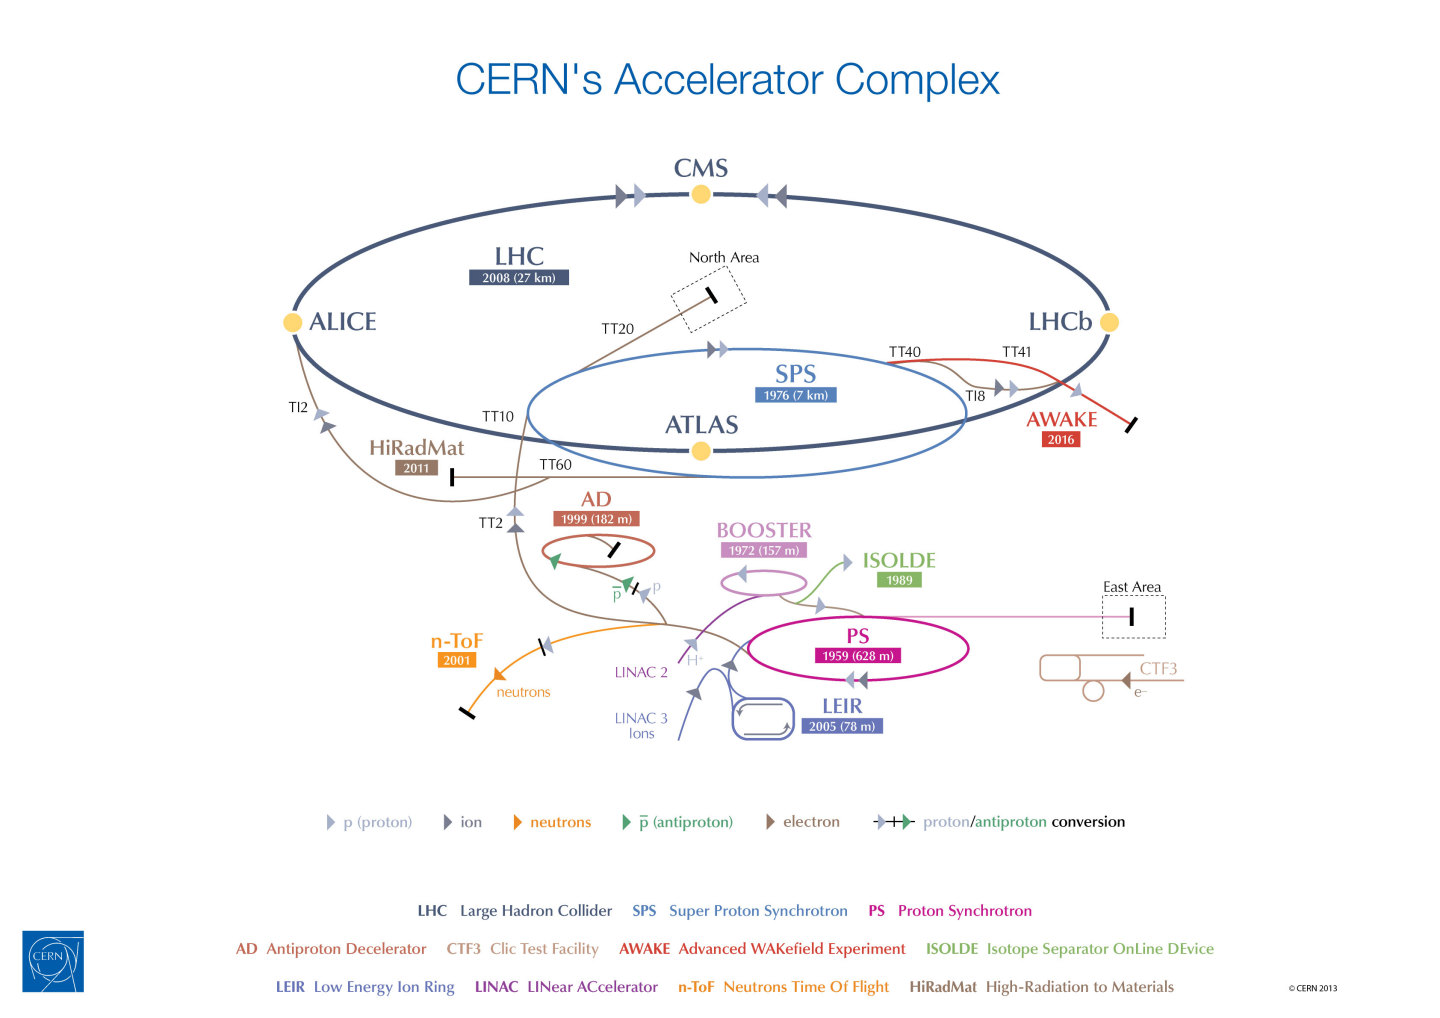
\includegraphics[width=6in]{images/cern_accel_complex.png}
  \caption
   {The CERN Accelerator Complex \cite{cernaccelcomplex}}
  \label{fig:cernaccel}
\end{figure}

First, the protons are created from a source of Hydrogen gas. The hydrogen atoms of the gas are placed into a large electric field that separates the atoms into unbound protons and electrons. The protons are then sent to a radio frequency quadrapole which focuses the protons and accelerates them. The radio frequency field is stronger for the protons in the back than in the front and consequently squeezes them into a tighter bunch. The protons then proceed to a linear accelerator, LINAC2, where they are accelerated to 50 MeV or 5\% of the speed of light (c). The protons then enter a series of synchrotrons. A synchrotron is a device that accelerates particles by guiding them around a fixed circular path with a magnetic field and boosting their speed with an electric field as they pass a certain point. Since a faster particle bends less in the same magnetic field, the magnetic field strength is synchronized with the speed of the accelerating particles to keep them in the fixed circular path. 

After LINAC2 the protons enter the first of the synchrotrons, the Proton Synchrotron Booster (PSB) accelerating the protons to 1.4 GeV (0.81c). From here the protons are injected into the Proton Synchrotron (PS) and accelerate to 25 GeV (0.999c). The PS then injects the protons into the Super Proton Synchrotron (SPS) further accelerating them to 450 GeV (0.99999c). Finally the protons are injected into the LHC where they accelerate up to 6.5 TeV (0.99999999c). Once accelerated to the appropriate collision energy, the proton beams are made to collide in the different detectors located around the ring. By colliding enough protons at large enough energies it is possible to probe corners of physics that have never been seen before. The two general purpose detectors at the LHC, ALTAS and CMS, are used to look for signs of new physics like the Higgs boson, dark matter, and extra dimensions by measuring the energy, the momentum, and the paths of the particles coming out of the collisions.

\section{Compact Muon Solenoid Detector}

The CMS detector, located in Cessy, France, is 21.6 m long, 15 m in diamater, and weighs more than the Eiffel Tower. Not only is the detector a massive and complex device it's also run by a huge collaboration involving approximately 3,800 people from 200 institutes spanning 43 different countries \cite{cmscollab}. The greatest achievement of the collaboration to date is the discovery of a Higgs like particle in 2012, a feat shared with ATLAS.

\begin{figure}[h!]
  \centering
  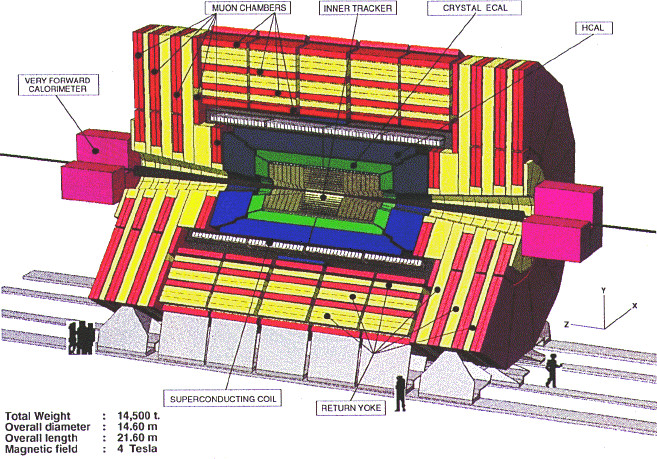
\includegraphics[width=4in]{images/CMSdetc3D.jpg}
  \caption
   {The CMS detector \cite{cmsweb}}
  \label{fig:cmsdet3d}
\end{figure}

CMS was built primarily to look for the Standard Model Higgs and signs of Beyond Standard Model (BSM) physics like Supersymmetry, extra dimensions, or new heavy weak bosons \cite{tdr}. Because BSM and Higgs decays to muons and electrons often have the highest signal to background ratio, CMS is designed to identify and measure these particles with a high accuracy. In layman's terms a high signal to background ratio just means that these events have fewer look-alikes. Jets \footnote{When a quark or gluon is created it can't exist alone, since it has color charge, and pulls other quarks from the vacuum creating a tight cone of composite colorless particles as well as their decays. This cone of particles is called a jet.} and photons are measured to a high degree of accuracy as well. In order to measure the energy, momentum, and location of the different types of particles CMS deploys a variety of subdetectors working in concert. The defining feature of the detector is an extremely powerful solenoid which enables the accurate measurement of momentum for charged particles. The tracker and calorimeters fit snugly within the 6 m diameter solenoid. The muon detectors reside outside the magnet but within the return yoke.

\subsection{Silicon Tracker}
The 3.8T magnetic field inside the solenoid enables the tracker to measure the transverse momentum of charged particles based upon the curvature of the track. Charged particles with lower transverse momentum ($p_{t}$) bend more in a magnetic field than high $p_{t}$ particles. As such, a measurement of the deviation of a curved track from a straight line, the sagitta, can be used to measure the curvature and determine the momentum \cite{pdgreview}.

\begin{equation}
p_{t} \cong \frac{L^{2}qB}{8s}
\end{equation}

Here L is the length of the straight line between the first and last position measurments, q is the charge of the particle, B is the magnetic field, and s is the sagitta.

\begin{figure}[h!]
  \centering
  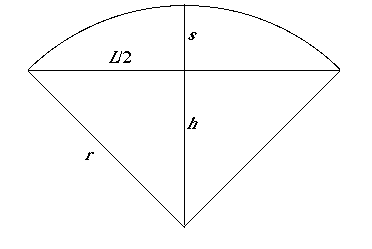
\includegraphics[width=3in]{images/sagitta.png}
  \caption
   {The sagitta measurement}
  \label{fig:sagittadrawing}
\end{figure}

The equation for the error in the momentum measurement shows that a higher magnetic field enables better $p_{t}$ resolution, illuminating the design choice for a powerful magnet.

\begin{equation}
\frac{\delta p_{t}}{p_{t}} \propto \frac{p_{t}}{L^{2}B} 
\end{equation}

The silicon tracker is made of tiny reverse biased bipolar diodes. When a charged particle travels through one of these diodes the ionization force of the particle releases electron hole pairs beyond the electrostatic equilibrium, inciting a current to flow. The tracker needs to be small enough such that the particles flowing through it don't deposit much energy. Energy deposition in the tracker would throw off energy measurements in the calorimeters. This means that the tracker needs to be smaller than a few radiation lengths \footnote{the length scale over which an electron deposits a substantial amount of energy into the material}. The tracker at the thickest part is one radiation length. The tracker is placed nearest the collision point in order to identify primary and secondary vertices and to measure the momentum of particles before they are tainted by interactions with other detectors. \footnote{Vertex is shorthand for the location of the collision or decay that produced a set of particles.} Being so near the collision point, the silicon tracker is bombarded by a constant flux of high intensity radiation. As such, the tracker is carefully designed to be robust to this radiation rich environment.

\subsection{Calorimeters}
The Electromagnetic Calorimeter (ECAL) is right outside the tracker and its main goal is to measure the energy of electrons and photons. It's designed to contain entire electromagnetic showers for these particles and is consequently many radiation lengths thick. The ECAL is made of lead tungstenate scintillating crystals which release an amount of light proportional to the energy deposition. The light is collected and the total energy is calculated. The separation into individual crystals allows some spatial resolution as well. Particles with larger mass deposit less energy per unit distance into a solid. Many of the hadronic particles make it through the ECAL for this reason.

\begin{figure}[h!]
  \centering
  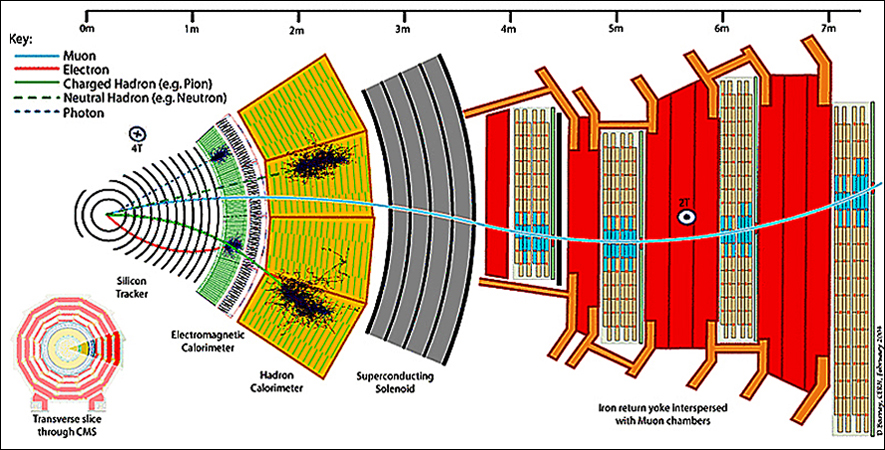
\includegraphics[width=4in]{images/cms_slice.jpg}
  \caption
   {A slice of the CMS detector \cite{cmsweb}}
  \label{fig:cmsdetslice}
\end{figure}

The HCAL is placed outside the ECAL to collect the energy of the particles that survived the other subsystems, mostly strongly interacting hadronic particles from jets. The HCAL works in a similar manner to the ECAL except that layers of plastic scintillating material are interspersed with layers of a dense passive absorber like brass or steel. The density of the passive absorber increases the chance of interaction and shower production thus reducing the total length of the hadronic shower and enabling the measurement of the total energy for most of the cascades. Again the scintillation light is collected to determine the energy. If the ECAL and HCAL were placed outside the magnet the particles would interact with the solenoid material before entering the calorimeters, throwing off their measurements. The showers in the calorimeters are a consequence of the electromagnetic and strong forces, which means that particles without these interactions pass through the materials undetected, e.g. neutrinos or BSM weakly interacting particles. Since the momentum in an interaction is conserved any imbalance means that some particles escaped the detector. If there is an excess of missing momentum beyond the amount expected due to neutrinos this may indicate the existence of dark matter or some other BSM particle. In order to measure the missing energy correctly it's important that the HCAL is built without any gaps and that it is dense enough to collect the energy of the strongly and electrically interacting particles.

While the momentum resolution in the tracker is proportional to the momentum, the energy resolution in the calorimeters decreases with increasing energy \cite{pdgreview}.

\begin{equation}
\frac{\delta E}{E} = \sqrt{\left(\frac{S}{\sqrt{E}}\right)^2 + \left(\frac{N}{E}\right)^2 + C}
\end{equation}

The first term in the square root describes statistical fluctuations. The energy measured is proportional to the number of photons captured which has poisonnian fluctuations and the error (${\rm \delta E}$) for this term is $\propto \sqrt{{\rm E}}$. The second term describes noise in the electronics whose error is energy independent, and the last term describes the errors in energy calibration which are proportional to energy.

\subsection{Muon System}
Neutrinos aren't the only Standard Model particles that make it through the tracker, ECAL, and HCAL. Muons have a relatively long lifetime $\sim 10^{-6} s$  with $c\tau \sim 100 m$. The large gamma factor in combination with their long lifetime enables them to travel hundreds of kilometers on average, well through the entire CMS detector before decaying. Muons are charged so their tracks show up in the tracker and some energy is deposited in the calorimeters but, muons are so much more massive than electrons that the energy deposition in the ECAL is minimal. Making it through the ECAL the muons enter the HCAL. The HCAL is designed to stop strongly interacting hadronic particles and collect their energy. But muons don't interact with the strong force and make it through the HCAL as well. This enables the muon system to be placed outside the magnet.

The muon system consists of a few different types of detectors which all involve the same basic principle. The charged muon ionizes some gas and the ionized particles are attracted to charged surfaces initiating a current in the surfaces. With a large enough voltage differential between the charged surfaces the the ionized particles may gain enough kinetic energy to further ionize other atoms in the gas initiating an avalanche effect and reducing the need for signal amplification later. The muon system uses this strategy in the different detectors. The types of detectors in the muon system are the Cathode Strip Chambers (CSC), the Drift Tubes (DT), and the Resistive Plate Chambers (RPC) \cite{tdr}.

\begin{figure}[h!]
  \centering
  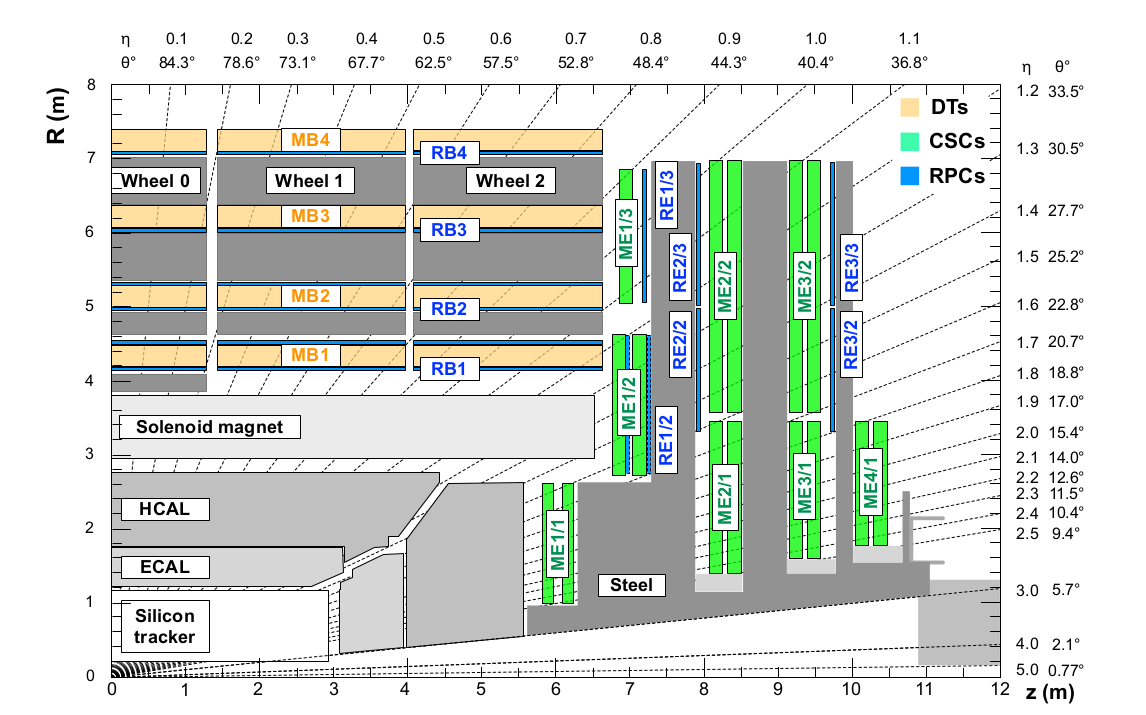
\includegraphics[width=5.5in]{images/muon_system.png}
  \caption
   {A Look at the Muon System \cite{muonsys}}
  \label{fig:muonsysfig}
\end{figure}

\newpage

\subsubsection{Drift Tubes}

The drift tubes are located in the barrel portion of CMS. Throughout the majority of the barrel the magnetic field is basically uniform. The drift tubes have aluminum plates on the top and bottom separated by aluminum I-beams shown in Figure ~\ref{fig:dt}. A wire acts as the anode and the I-beams are the cathodes. The tubes are designed to provide a constant drift velocity throughout each tube.

\begin{figure}[h!]
  \centering
  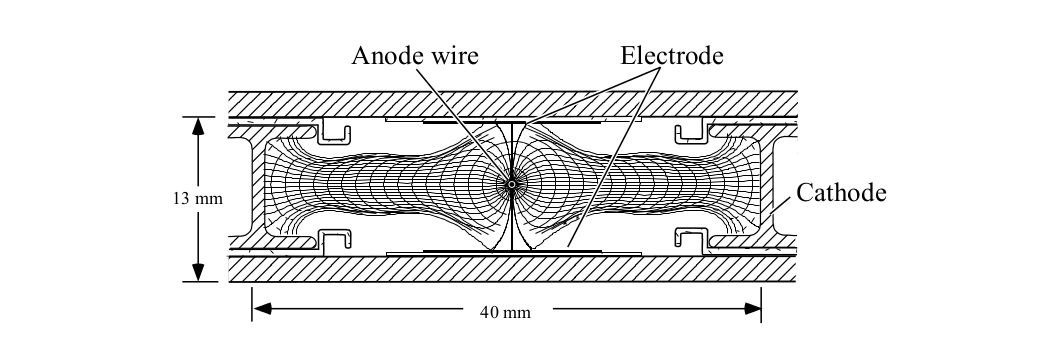
\includegraphics[width=4in]{images/DT.png}
  \caption
   {A Drift Tube \cite{mutdr}}
  \label{fig:dt}
\end{figure}

When a charged particle flies through the tube it ionizes the gas inside. The electrons drift at constant velocity to the anode. The distance from the anode is deduced from the drift time, utilizing the fact that the ionized electrons drift with a constant velocity. This calculation does however require a reference time. In each chamber the drift tubes are placed in layers and the average crossing time in the chamber is used as the reference time.

\subsubsection{Cathode Strip Chambers}

The CSCs are located in the endcaps of the detector which range in $|\eta|$ from 0.8 to 2.4. One of the reasons the endcaps use CSCs instead of DTs is the nonuniform magnetic field which would adversely affect the drift times in the DT system. In this system there are oppositely charged strips and wires running roughly perpendicular to eachother.

\begin{figure}[h!]
  \centering
  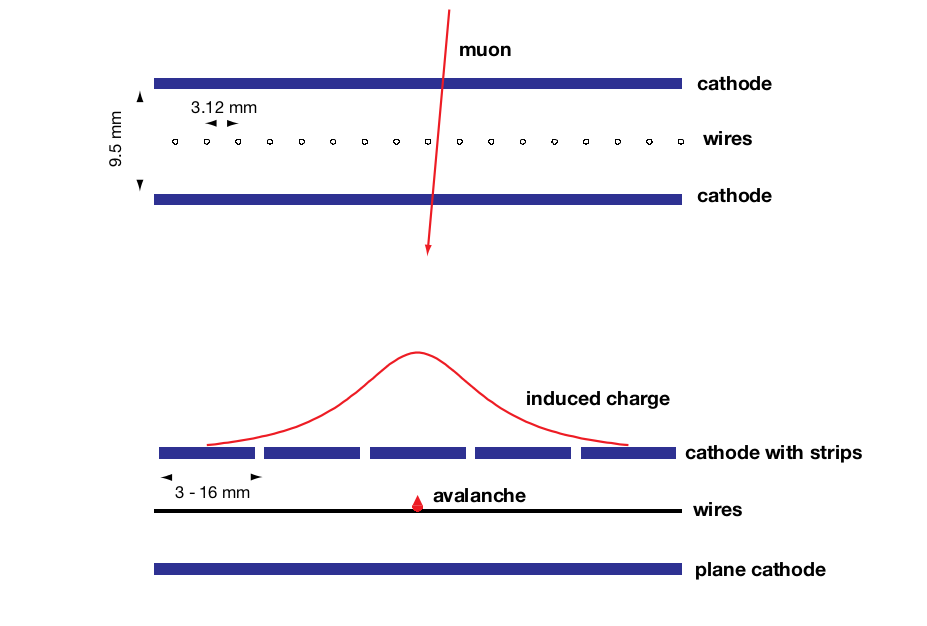
\includegraphics[width=4in]{images/CSC.png}
  \caption
   {A Cathode Strip Chamber \cite{mutdr}}
  \label{fig:csc}
\end{figure}

When a muon flies through the CSC it induces charge on the wires and the strips and ionizes gas in the chamber. The ionized particles in the gas float to the charged strips and wires initiating a current in the nearby wires and strips. The induced charge from the muon itself also contributes to the currents. The most intense currents should be those associated with the location of the muon. The position resolution in the phi direction is roughly 100 ${\rm \mu m}$.

\subsubsection{Resistive Plate Chambers}

The RPCs are located both in the barrel and in the end caps. The RPCs have excellent timing resolution on the order of 1 ns. The RPCs use their excellent timing resolution to determine each particle's bunch crossing of origin. The accurate and rapid timing information helps with the online selection of muons, a huge priority for CMS considering that many interesting collisions produce muons. For this reason the RPCs focus on efficient online selection of muons instead of accurate offline reconstruction \cite{cmsexp}.

In this way the RPCs complement the DTs and CSCs. The RPCs consist of two high resistance parallel plates surrounding a volume of gas. The outsides of the plates are painted with graphite paint forming the electrodes. A large voltage differential is kept between the electrodes. When a charged particle crosses the plates it induces an electrical discharge in the plates which remains localized in time and space due to the large resistivity.

\subsection{Trigger System}
Collision events come at a rate of 10 MHz with each event taking up roughly a MB of information. If the detector had to store all of the information from each event this would amount to pushing terabytes of information into a storage system every second, which is remarkably infeasible. To deal with this issue CMS utilizes a trigger system, which selects only interesting events cutting the rate down from 10 MHz to 1 KHz \cite{cmsexp}. Since bunch crossings happen every 25 ns the trigger needs to operate at an incredibly high rate.

CMS tackled this issue by dividing the trigger into different tiers. The Level 1 Trigger is the first stage of the trigger system made from custom hardware which can operate at fantastic speed. The Level 1 Trigger reduces the rate from 10 MHz to 100 KHz and the events passing the L1 Trigger go onto the High Level Trigger (HLT) which further reduces the rate to 1 KHz. Due to the lower input rate the HLT can operate in software.

\subsubsection{L1 Trigger}

The L1 Trigger is made of up different subsystems that work together to decide whether to keep the data from a beam crossing for further processing. The University of Florida works with the Level 1 muon trigger system, the Endcap Muon Track Finder (EMTF) in particular. The muon system needs to determine the transverse momenta of muons and their location and choose the best candidates. Each of the different muon detectors have their own local triggers which send their best muon tracks to the Global Muon Trigger (GMT). The GMT chooses the best muon candidates from that set and passes these on to the Global Trigger (GT). The GT combines the information from the calorimeter triggering system. The GT uses this combined information to check whether the bunch crossing should be sent to the HLT or discarded. The L1 Trigger has many different trigger criteria defining separate triggers which are the trigger bits. If an event passes any of the triggers then it is forwarded for further processing.

\begin{figure}[h!]
  \centering
  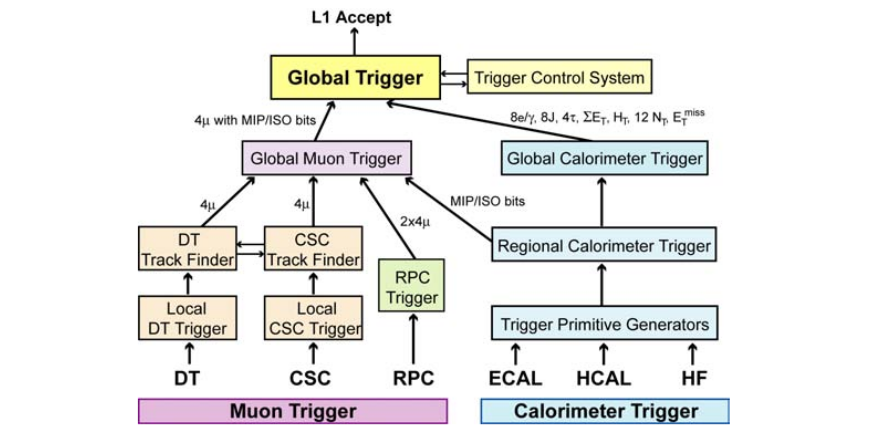
\includegraphics[width=5in]{images/L1_Trigger.png}
  \caption
   {The L1 Trigger Architecture \cite{cmsexp}}
  \label{fig:l1trigarch}
\end{figure}

The Track Finders (TF) play an important role in the L1 Trigger system. The EMTF combines the location and direction information from the different CSC stations into muon tracks and calculates the transverse momenta for the different tracks. The EMTF chooses the best candidates (highest momentum and highest quality) to send to the GMT. The Drift Tube Track Finder (DTTF) performs a similar process for muons in the DT system. The RPC system calculates the location and direction and forms tracks in the same stage. In the process the RPC trigger system assigns transverse momenta and quality, and like the others chooses the best tracks to send to the GMT.

\chapter{THE STANDARD MODEL} \label{sm}

The Standard Model (SM) of particle physics is an incredibly successful theory that correctly describes the physics of all known particles and forces that make up the universe, excluding gravity \cite{smconsistency}. The particles of the SM come in two types, fermions and bosons \footnote{Bosons have integer spin.}. Fermions are the spin 1/2 particles and make up the different types of matter. Electrons are a familiar example, and the up and down quarks that make up protons and neutrons are others. While electrons and the up and down quarks account for nearly all of the matter in our day to day experience there are actually many other fermions. In fact, there are three generations of quarks and leptons \footnote{Leptons are fermions that aren't quarks.} with each generation heavier than the next. The up and down quarks are the first generation of quarks, charmed and strange are the next, and top and bottom are the third generation. For the leptons the electron and electron neutrino are the first generation, the muon and muon neutrino are the second, and the tau and the tau neutrino the third. Each fermion also has a corresponding antiparticle. As an example, the positron is the antiparticle for the electron. 

\begin{figure}[h!]
  \centering
  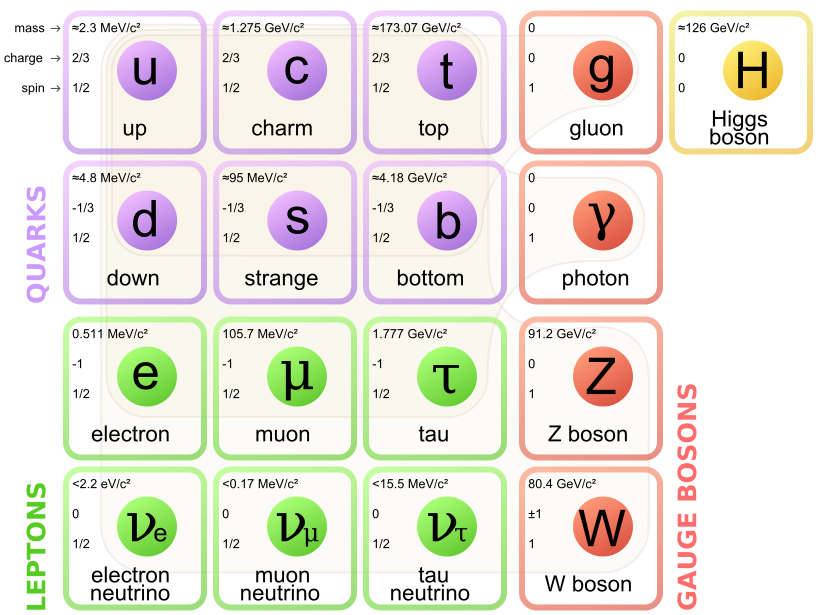
\includegraphics[width=4in]{images/Standard_Model_of_Elementary_Particles.png}
  \caption
   {The Standard Model Particles}
  \label{fig:smtable}
\end{figure}

The universe would be pretty boring if the particles couldn't attract or repel or form more complex objects like atoms, molecules, and even people. Luckily there are forces as well and these forces are described by the spin 1 bosons. The fermions attract and repel by exchanging bosons, which is why the bosons are often called force carriers. Gluons mediate the strong force, photons the electromagnetic force, and the W and Z bosons mediate the weak force. Every force has an associated charge. Just as those particles with electric charge can interact through the electromagnetic force, those with color charge may interact via the strong force, and those with isospin may interact through the weak force. The fundamental forces and particles interact to make the familiar composite objects that surround us in our daily lives. The strong force binds quarks to form protons and neutrons, the Van Der Waals version of the strong force binds the protons and neutrons together to form nuclei, and the electromagnetic force binds electrons and nuclei to form atoms. The size of the composite objects gives an idea of the relative strength of the forces. A proton is ~$10^-15$ meters in size while an atom is ~$10^-10$ meters and a solar system is ~$10^12$ meters. The more tightly bound the stronger the force. In fact the ratio of the strength of the forces is like so 1:$10^-3$:$10^-16$:$10^-41$, strong : electromagnetic : weak :gravitational \footnote{Gravity is just included for perspective. The Standard Model does not describe this force and reconciling gravity with quantum mechanics is an open problem.}. 

Of all the particles predicted by the SM, only the Higgs boson remains to be found. The Higgs boson is the only spin 0 particle of the SM. It is theorized that as the universe cooled from the Big Bang the Higgs field went through a phase transition and settled into a nonzero ground state forming a condensate. And it is the potential energy from the interactions with this nonzero ground state that give the massive fundamental particles their mass. With such a large role in the SM, finding this particle or a BSM Higgs has been a huge priority for the CMS collaboration \cite{tdr}. In 2012 a Higgs particle with a mass of 125 GeV was found and to date remains consistent with the Standard Model. However, the properties need to be investigated further before declaring the discovered Higgs the Higgs of the Standard Model. 


%%%%%%%%%%%%%%%%%%%%%%%%%%%%%%%%%%%%%%%%%%%%%%%%%%%%%%%%%%%%%%%%%%%%%%%%%%%

\section{Quantum Field Theory}


The mathematical framework used to describe the physics of the SM as well as other Beyond Standard Model (BSM) field theories is called Quantum Field Theory (QFT). QFT enables the predictions of measurable quantities, namely the probabilities for different sets of particles to come out of a specific collision or for a single particle to decay into different sets of particles. These probabilities are encompassed in the cross sections and branching fractions. For example, the theory of the SM predicts the cross section for two protons colliding and making a Higgs. As another example, the SM also predicts the branching fraction for a Z boson decaying to two muons. These probabilities can be measured simply by colliding particles and counting the outcomes which in turn means that the theory can be tested. In fact, any QFT model can be tested in this manner. There are other commonly measured properties as well like the lifetime, spin, and mass of different particles.  

\subsection{What is a Particle?}

Since QFT makes quantitative predictions in terms of particle collisions and particle decays it's interesting to contemplate what a particle really is. The idea of a particle is often taken for granted. Consider an observer in a frame x with particle p and an observer in another frame x'. If the observer in x' can't identify particle p then it doesn't make sense to call p a particle. More concretely, consider a world where in frame x an observer sees a neatly stacked deck of cards, but in x' the observer sees the cards scattered all over the place. Calling the deck of cards a particle doesn't really make sense. On the other hand, both parties can still agree on the individual cards which kept the same suit and value. These are conserved quantities. If the two observers get together later and compare notes they can see what happened to each card upon transforming from x to x' and work out a set of rules. The king of hearts may do one thing and the 10 of clubs another. They can then add the different forces into play repeat the process and compare again. Figuring this all out determines the laws of physics for the fundamental pieces called particles.       

This idea leads to Wigner's view: a particle is an object with conserved quantities that observers can agree on between frames. In our universe these labels are the mass, charge, spin, color, and isospin. And because different observers can agree on these quantities they can compare notes and work out the laws of physics for the different types of particles. All that remains is to work out laws that people in different frames can confirm, and this is where the Lagrangian formalism comes into play. 

\subsection{The Lagrangian Formalism}

The Lagrangian formalism is a mathematical device that allows physicists to describe the evolution of a physical system over time, and it's within this formalism that QFT can be built. But before building the full mathematics of QFT, a simple example of the free Newtonian particle is given, and the different symmetries are observed. The Newtonian example serves as a starting point, and eventually the theory of the Standard Model will be developed using the symmetries as a roadmap. The fact that the laws of physics are indistinguishable in different inertial frames along with the requirement that the speed of light remain constant in all frames of reference lay the foundation for QFT. 

So let's get into the framework. The goal of physics is to describe how a physical system evolves over time, and this evolution is usually given by some differential equation describing the state the system will take in the next interval of time given the current time. Moving from state to state from one interval of time to the next, the system traces out a path in space and time or some other more abstract space of possible states. So how does one get the appropriate differential equation? As it turns out nature tries to minimize the difference between the energy spent \footnote{Spent here just means used as kinetic energy.} and the energy available to spend and it minimizes the action S. In the equation below, L is the Lagrangian, T is the kinetic energy and U is the potential energy.     
\begin{equation}
S = \int L dt = \int T - U dt
\end{equation}

At an extremum of S, $\delta S$ = 0 since S must go down then through a slope of zero and back up or vice versa. This assumes continuity and must be true for all parameters -- all directions. So to get the equations of motion just vary the parameters of L and solve for the values that yield zero change in the action.

\begin{equation}
\delta S = \int L(z_1 + dz_1, z_2+dz_2, ...)dt - \int L(z_1, z_2, ...)dt 
\end{equation}

Following this process yields the Euler-Lagrange (differential) equations, describing how the parameters z evolve over time. The z's may be the position and velocity, or the quantum fields, or the temperature and volume or some other set of parameters that describe the system. The Lagrangian for a Newtonian free particle in one dimension is pretty simple and gets the point across. 

\begin{equation}
S = \frac{1}{2} \int m\dot{x}^2 dt
\end{equation}

If the action is at an extremum, perturbing the path x(t) by adding the infinitesimal $\epsilon$(t) leaves the action unchanged.

\begin{equation}
S' = \frac{1}{2} \int m(\dot{x} + \dot{\epsilon})^2 dt = \frac{1}{2} \int m(\dot{x}^2 + 2\dot{x}\dot{\epsilon} + \dot{\epsilon}^2) dt =  
\frac{1}{2} \int m(\dot{x}^2 + 2\dot{x}d\dot{x}) dt 
\end{equation}

\begin{equation}
\delta S = S' - S = 0 = \frac{1}{2} \int m(\dot{x}^2 + 2\dot{x}\dot{\epsilon}) dt - \frac{1}{2} \int m\dot{x}^2 dt = \int m\dot{x}\dot{\epsilon} dt
\end{equation}

Since x(t) is fixed at the boundaries of the integral, $\epsilon$ must be zero at $t_o$ and $t_f$, so integrating by parts yields the following equation. 

\begin{equation}
\delta S = 0 = \epsilon(t_f) \dot{x}(t_f)  - \epsilon(t_o) \dot{x}(t_o) + \int m\ddot{x} \epsilon dt  = 
0\dot{x}(t_f)  - 0\dot{x}(t_o) + \int m\ddot{x} \epsilon dt = \int m\ddot{x} \epsilon dt
\end{equation}

And this equation must be zero for any infinitesimal deviation $\epsilon$.

\begin{equation}
\delta S = 0 \rightarrow m\ddot{x} = 0
\end{equation}

So a free particle keeps the same velocity over time. Note that a Newtonian boost by constant velocity $v \rightarrow v' = v + u$ \footnote{Renaming $\dot{x}$ as v.} leaves the equations of motion consistent. In the unprimed frame the particle has velocity v with 0 acceleration. In the primed frame the particle has velocity v + u with 0 acceleration. Both observers see the particle act as if there are zero forces.

\begin{equation}
S = \frac{1}{2} \int m(v + u)^2 dt  =  \frac{1}{2} \int m(v')^2 dt \rightarrow \delta S = 0 \rightarrow m\frac{d}{dt}(v+u) = m\frac{d}{dt}(v') = 0 
\end{equation}

If u is not constant but a function of time u(t) then the equations of motion do not describe the same time evolution.

\begin{equation}
m\frac{d}{dt}(v+u) = m\dot{v} + m\dot{u} = 0 \rightarrow \dot{v} = -\dot{u}
\end{equation}

In the case where u(t) depends upon time, the difference between the primed and unprimed frames' equations of motion is then $\delta F$.

\begin{equation}
\delta F = m\frac{d}{dt}(v+u) - m\frac{dv}{dt} = m\dot{v} + m\dot{u} - m\dot{v} = m\dot{u}
\end{equation}

In the unprimed frame, the particle identified by the mass moves with constant velocity, $\dot{v} = 0$. The observer in the primed frame looks at the particle with the same mass and sees it change velocity given by the equation $\dot{v} = -\dot{u}$. As an example, set v and $u, \dot{u}$ to zero for all times before t=0, and let $u, \dot{u}$ turn on after time 0. Both observers will agree that the particle is stationary up until time 0. After which, the observer in the primed frame will see the particle accelerate in strange ways. Meanwhile, the unprimed frame will continue to observe a stationary particle. 

In general, every inertial frame finds $\delta F = 0$ and every accelerating frame finds an extra force $\delta F$ unique to its acceleration. In this way no observer in an inertial frame can perform an experiment and determine which inertial frame he or she is in. On the other hand, each accelerating frame is identified by its $\delta F$.  In every inertial frame a ball released at rest remains at rest. In an accelerating frame the ball will accelerate according to the motion of the frame $\delta F$ and this change in the laws of physics identifies the frame in a unique way. Conversely, the laws of physics remain the same boosting between inertial frames, and this invariance is a symmetry of physics. Of course this example is Newtonian and the correct way to boost is given by the Lorentz transformation from Special Relativity, but this gets the point across.

Delving further along the path of symmetry, the fundamental forces depend only on the distance from the charge and not the direction implying that rotations are also a symmetry. This can be seen by looking at the Lagrangian. 

\begin{equation}
L = \frac{1}{2} m\dot{\vec{x}}^2 - U((\vec{x} - \vec{x'})^2)
\end{equation}

Rotations leave dot products and consequently the magnitude of vectors unchanged so the Lagrangian is invariant under this transformation. Naturally if the Lagrangian is invariant the equations of motion will be as well.

\begin{equation}
m\frac{d\vec{v}}{dt} = \vec{\nabla} U
\end{equation}

In the equations of motion above, both sides are vectors and vectors transform the same way under rotations so the equations of motion are invariant. Note that in the case of rotations both the Lagrangian and the equations of motion are invariant. While for Newtonian boosts only the equations of motion were invariant. This is due to the fact that Newtonian mechanics is the low velocity limit of relativistic mechanics. In the theory of Special Relativity the action for a massive free particle is written like so.

\begin{equation}
S = \int \frac{m}{2}u^{\mu}u_{\mu}d\tau
\end{equation}

Just as rotations preserve the dot product, Lorentz transformations (boosts and rotations) preserve the four vector product. Insofar, both the relativistic Lagrangian and the resulting equations of motion remain invariant under a boost or rotation to a new inertial frame. Building the Lagrangian out of four vector products gaurantees this. Interestingly enough, by studying the properties of the Lorentz group it's possible to find even more fundamental building blocks called spinors.

\subsection{QFT From Symmetry}

The laws of physics are invariant under boosts and rotations, and the Lagrangian provides a mathematical framework for physical predictions. These facts together imply that there's a good shot at building a proper QFT by creating the appropriate invariant Lagrangian. Four vector products remain invariant under Lorentz transformations so they are a natural ingredient, but there are other mathematical objects that could be used as well. In this vein, the symmetries under rotations and boosts are investigated in order to look for some other building blocks. The goal is to find two different representations of the Lorentz group and use one representation to describe fermions and other for bosons.

\subsubsection{Rotations}

Rotations in three dimensions are described by the SO(3) group. Rotations preserve the lengths of vectors and the angles between them, which means that dot products between vectors remain invariant as well. In three dimensions one can rotate about any of the three axes. The rotations about the x, y, and z axes may be characterized by the matrices below.

\begin{equation}
R_x = 
\begin{pmatrix}
1 & 0 & 0 \\
0 & \cos\theta_x & -\sin\theta_x \\
0 & \sin\theta_x & \cos\theta_x \\
\end{pmatrix}
\end{equation}

\begin{equation}
R_y = 
\begin{pmatrix}
\cos\theta_y & 0 & \sin\theta_y \\
0 & 1 & 0 \\
-\sin\theta_y & 0 & \cos\theta_y \\
\end{pmatrix}
\end{equation}

\begin{equation}
R_z = 
\begin{pmatrix}
\cos\theta_z & -\sin\theta_z & 0 \\
\sin\theta_z & \cos\theta_z & 0 \\
0 & 0 & 1 \\
\end{pmatrix}
\end{equation}

These rotations may be built up from repeated rotations by an infinitesimally small angle $d\theta$. The matrices characterizing an infinitesimal rotation are given by taking the limit as $\theta$ goes to zero.

\begin{equation}
dR_x = 
\begin{pmatrix}
1 & 0 & 0 \\
0 & 1 & -d\theta_x \\
0 & d\theta_x & 1 \\
\end{pmatrix}
= 1 - id\theta_x
\begin{pmatrix}
0 & 0 & 0 \\
0 & 0 & -i \\
0 & i & 0 \\
\end{pmatrix}
= 1 - id\theta_x J_x
\end{equation}

\begin{equation}
dR_y = 
\begin{pmatrix}
1 & 0 & d\theta_y \\
0 & 1 & 0 \\
-d\theta_y & 0 & 1 \\
\end{pmatrix}
= 1 - id\theta_y
\begin{pmatrix}
0 & 0 & i \\
0 & 0 & 0 \\
-i & 0 & 0 \\
\end{pmatrix}
= 1 - id\theta_y J_y
\end{equation}

\begin{equation}
dR_z = 
\begin{pmatrix}
1 & -d\theta_z & 0 \\
d\theta_z & 1 & 0 \\
0 & 0 & 1 \\
\end{pmatrix}
= 1 - id\theta_z 
\begin{pmatrix}
0 & -i & 0 \\
i & 0 & 0 \\
0 & 0 & 0 \\
\end{pmatrix}
= 1 - id\theta_z J_z
\end{equation}

Repeating an infinitesimal rotation many times rebuilds the finite rotation, so the J matrices generate rotations along their respective axes and they are aptly referred to asthe generators of the group. Some algebra reveals this to be the case.

\begin{equation}
R = (1 - i\frac{\theta}{N} J)^{N} = 1 + (-id\theta J) + \frac{1}{2!}(-id\theta J)^2 + \frac{1}{3!}(-id\theta J)^3 + ... = e^{-i\theta J} 
\end{equation}

Notice that even powers of J yield $J^2$ and that odd powers of J return J.

\begin{equation}
  = 1 - J^2 + J^2(1 + \frac{i^2}{2!} d\theta^2 + \frac{i^4}{4!} d\theta^4 + ...) - iJ(d\theta + \frac{i^2}{3!}d\theta^3 + \frac{i^4}{5!}d\theta^5 + ...) 
  = (1-J^2) + J^2 \cos\theta - iJ\sin\theta
\end{equation}

Plugging in $J_z$ reveals that this process does in fact rebuild the rotation matrix $R_z$.

\begin{equation}
\begin{split}
R_z &= 
(\begin{pmatrix}
1 & 0 & 0 \\
0 & 1 & 0 \\
0 & 0 & 1 \\
\end{pmatrix}
-
\begin{pmatrix}
1 & 0 & 0 \\
0 & 1 & 0 \\
0 & 0 & 0 \\
\end{pmatrix})
+
\begin{pmatrix}
1 & 0 & 0 \\
0 & 1 & 0 \\
0 & 0 & 0 \\
\end{pmatrix}
\cos\theta_z
+
\begin{pmatrix}
0 & -1 & 0 \\
1 & 0 & 0 \\
0 & 0 & 0 \\
\end{pmatrix}
\sin\theta_z
\\ &=
\begin{pmatrix}
\cos\theta_z & -\sin\theta_z & 0 \\
\sin\theta_z & \cos\theta_z & 0 \\
0 & 0 & 1 \\
\end{pmatrix}
\end{split}
\end{equation}

Similarly, the other generators rebuild their respective rotation matrices. The generators of the group are actually more fundamental than the rotation matrices. The multiplication table for the generators describes the algebra of the group, which describes the behavior of rotations at a local level. In fact the rotation matrices are just one of the groups with this local algebra, and a specific group obeying the local algebra is analagous to a specific solution of a differential equation: each solution has a different global behavior yet each obeys the same physics. Moreover the multiplication table can be specified without declaring any particular representation for the generators. 

\begin{equation}
\begin{split}
&J_x*J_y = iJ_z  + J_y*J_x \\
&J_y*J_z = iJ_x  + J_z*J_y \\
&J_z*J_x = iJ_y  + J_x*J_z \\
\end{split}
\end{equation}

The multiplication table can be specified in a more compact notation using the commutator, $[a,b] = ab - ba$, and the antisymmetric tensor $\epsilon$.
\begin{equation}
[J_k, J_l] = i\epsilon_{klm}J_m
\end{equation}

Finding 3x3 generators that obey the algebra and then repeatedly applying the infinitesimal transormations builds the SO(3) rotation group. The group acts on 3x1 objects called vectors, and these 3x1 vectors are a suitable candidate for a Newtonian Lagrangian. Finding another representation obeying this algebra will provide a more fundamental ingredient for the Lagrangian and allow the construction of a proper QFT. Similar to the way real numbers are built from the squares of imaginary numbers, vectors are built from spinors. 

Looking for the lowest order complex nxn matrices satisfying the algebra gives the 2x2 Pauli matrices. Any 1x1 matrices are simply scalar complex numbers, which commute and therefore cannot satisfy the algebra. The Pauli matrices are  

\begin{equation}
\sigma_x = 
\begin{pmatrix}
0 & 1 \\
1 & 0 \\
\end{pmatrix},
\sigma_y = 
\begin{pmatrix}
0 & -i \\
i & 0 \\
\end{pmatrix},
\sigma_y = 
\begin{pmatrix}
1 & 0 \\
0 & -1 \\
\end{pmatrix}
\end{equation}

However, plugging these into the commutator reveals a factor of two difference.

\begin{equation}
[\sigma_k, \sigma_l] = 2i\epsilon_{klm}\sigma_m
\end{equation}

Defining $J_k = \frac{1}{2} \sigma_k$ fixes this. These matrices act on an array of 2x1 complex numbers called spinors, and this new "rotation" group is called SU(2). Note that by starting with vectors and analyzing the SO(3) rotation group along with its underlying algebra, new mathematical objects have been discovered. It's now possible to use these spinors to build rotationally invariant Lagrangians. While rotationally invariant Lagrangians are important for nonrelativistic theories, the real goal is to break down four vectors in the same way to find the most fundamental ingredients for relativistic Lagrangians. 

\begin{equation}
[J_k, J_l] = i\epsilon_{klm}J_m
\end{equation}

\subsubsection{The Lorentz Group}
Four vector products are invariant with regards to rotations and boosts. This statement is defined by the mathematical equation below, where the $\Lambda$ matrices represent the rotation/boost matrices of the Lorentz Group and the $\eta$ matrix is the Minkowski metric $\left( \begin{smallmatrix} 1 & 0 & 0 & 0 \\ 0 & -1 & 0 & 0 \\ 0 & 0 & -1 & 0 \\ 0 & 0 & 0 & -1 \\ \end{smallmatrix} \right)$.

\begin{equation}
x'_{\mu} x'^{\mu} = x_{\mu} x^{\mu} \rightarrow \eta_{\sigma\rho} \Lambda^{\sigma}_{\mu}  \Lambda^{\rho}_{\nu} x^{\mu} x^{\nu} = \eta_{\mu\nu} x^{\mu} x^{\nu}
\rightarrow \eta_{\sigma\rho} \Lambda^{\sigma}_{\mu}  \Lambda^{\rho}_{\nu} = \eta_{\mu\nu}
\end{equation}

In this 3 + 1 dimensional space the rotations and their corresponding generators are now given by the following R and J matrices.

\begin{equation}
R_x = 
\begin{pmatrix}
1 & 0 & 0 & 0\\
0 & 1 & 0 & 0 \\
0 & 0 & \cos\theta_x & -\sin\theta_x \\
0 & 0 & \sin\theta_x & \cos\theta_x \\
\end{pmatrix},
J_x = 
\begin{pmatrix}
0 & 0 & 0 & 0\\
0 & 0 & 0 & 0 \\
0 & 0 & 0 & -i \\
0 & 0 & i & 0 \\
\end{pmatrix}
\end{equation}

\begin{equation}
R_y = 
\begin{pmatrix}
1 & 0 & 0 & 0\\
0 & \cos\theta_y & 0 & \sin\theta_y \\
0 & 0 & 1 & 0 \\
0 & -\sin\theta_y & 0 & \cos\theta_y \\
\end{pmatrix},
J_y = 
\begin{pmatrix}
0 & 0 & 0 & 0\\
0 & 0 & 0 & i \\
0 & 0 & 0 & 0 \\
0 & -i & 0 & 0 \\
\end{pmatrix}
\end{equation}

\begin{equation}
R_z = 
\begin{pmatrix}
1 & 0 & 0 & 0\\
0 & \cos\theta_z & -\sin\theta_z & 0 \\
0 & \sin\theta_z & \cos\theta_z & 0 \\
0 & 0 & 0 & 1 \\
\end{pmatrix},
J_z = 
\begin{pmatrix}
0 & 0 & 0 & 0\\
0 & 0 & -i & 0 \\
0 & i & 0 & 0 \\
0 & 0 & 0 & 0 \\
\end{pmatrix}
\end{equation}

And the boosts are given by the following B matrices.

\begin{equation}
B_x = 
\begin{pmatrix}
\cosh\omega_x & \sinh\omega_x & 0 & 0 \\
\sinh\omega_x & \cosh\omega_x & 0 & 0 \\
0 & 0 & 1 & 0 \\
0 & 0 & 0 & 1 \\
\end{pmatrix}
\end{equation}

\begin{equation}
B_y = 
\begin{pmatrix}
\cosh\omega_y & 0 & \sinh\omega_y & 0 \\
0 & 1 & 0 & 0 \\
\sinh\omega_y & 0 & \cosh\omega_y & 0 \\
0 & 0 & 0 & 1 \\
\end{pmatrix}
\end{equation}

\begin{equation}
B_z = 
\begin{pmatrix}
\cosh\omega_z & 0 & 0 & \sinh\omega_z \\
0 & 1 & 0 & 0 \\
0 & 0 & 1 & 0 \\
\sinh\omega_z & 0 & 0 & \cosh\omega_z \\
\end{pmatrix}
\end{equation}

Looking at the differential boosts yields the generators K.

\begin{equation}
dB_x = 
\begin{pmatrix}
1 & d\omega_x & 0 & 0 \\
d\omega_x & 1 & 0 & 0 \\
0 & 0 & 1 & 0 \\
0 & 0 & 0 & 1 \\
\end{pmatrix}
= 1 + d\omega_x 
\begin{pmatrix}
0 & 1 & 0 & 0 \\
1 & 0 & 0 & 0 \\
0 & 0 & 0 & 0 \\
0 & 0 & 0 & 0 \\
\end{pmatrix}
= 1 + d\omega_x K_x
\end{equation}

\begin{equation}
dB_y = 
\begin{pmatrix}
1 & 0 & d\omega_y & 0 \\
0 & 1 & 0 & 0 \\
d\omega_y & 0 & 1 & 0 \\
0 & 0 & 0 & 1 \\
\end{pmatrix}
= 1 + d\omega_y
\begin{pmatrix}
0 & 0 & 1 & 0 \\
0 & 0 & 0 & 0 \\
1 & 0 & 0 & 0 \\
0 & 0 & 0 & 0 \\
\end{pmatrix}
= 1 + d\omega_y K_y
\end{equation}

\begin{equation}
dB_z = 
\begin{pmatrix}
1 & 0 & 0 & d\omega_z \\
0 & 1 & 0 & 0 \\
0 & 0 & 1 & 0 \\
d\omega_z & 0 & 0 & 1 \\
\end{pmatrix}
= 1 + d\omega_z
\begin{pmatrix}
0 & 0 & 0 & 1 \\
0 & 0 & 0 & 0 \\
0 & 0 & 0 & 0 \\
1 & 0 & 0 & 0 \\
\end{pmatrix}
= 1 + d\omega_z K_z
\end{equation}

As before with the rotations in three dimensions the group is defined by its multiplication table. 

\subsubsection{Building Lagrangians}
\subsection{Perturbation Theory}
\subsection{Feynman Rules}

\begin{figure}[h!]
  \centering
  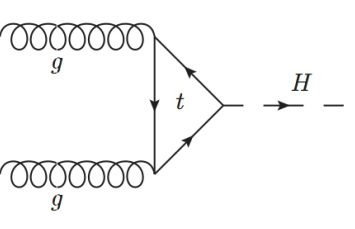
\includegraphics[width=1.5in]{images/ggf.png}
  \caption
   {The Feynman diagram for two gluons fusing into a Higgs. There are three vertices and this is a third order diagram. Two vertices involve the strong force and one vertex involves the Higgs coupling. The matrix element for this diagram would have two factors of the strong force coupling and one factor for the Higgs coupling which involves the mass of the top quark.}
  \label{fig:feynggf}
\end{figure}

%%%%%%%%%%%%%%%%%%%%%%%%%%%%%%%%%%%%%%%%%%%%%%%%%%%%%%%%%%%%%%%%%%%%%%%%%%%
\section{The Standard Model Higgs}


%%%%%%%%%%%%%%%%%%%%%%%%%%%%%%%%%%%%%%%%%%%%%%%%%%%%%%%%%%%%%%%%%%%%%%%%%%%
\subsection{SM Higgs Production and Decay Modes}

The SM Higgs can be created in a variety of ways. Some of these cross sections are shown below for 14 TeV collisions. The production cross sections are functions of the mass of the Higgs as well as the energy of the collisons. For a given collision energy the cross sections decrease as the Higgs mass increases: there are fewer kinematic possibilities for a heavier particle since more of the energy was used to create the particle. For a given mass, say 125 GeV, the cross section grows with collision energy. This constrasts with cross sections involving collisions of fundamental particles, e.g. electron antielectron collisions. This is an artifact of the fact that the LHC collides protons together. 

\begin{figure}[h!]
  \centering
  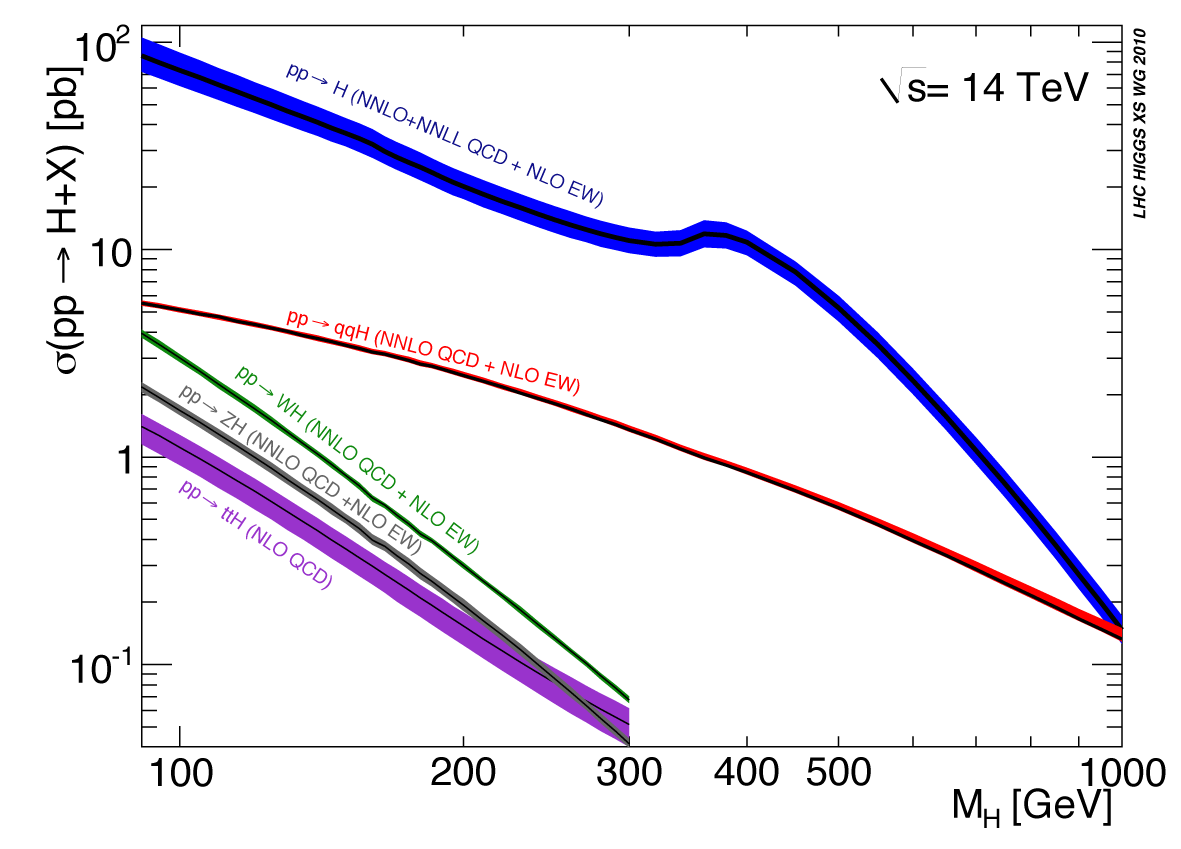
\includegraphics[width=5in]{images/14TeV_higgs_cross_sections.png}
  \caption
   {The highest production mode cross sections for the SM Higgs \cite{crossbranchplots}}
  \label{fig:hprodcross}
\end{figure}

Protons behave like a collection of an infinite number of quark-antiquarks, an infinite number of gluons, and the usual uud. The total momentum of the proton is divided up amongst them with lots of particles having little of the total momentum. The actual scattering events are between these more fundamental particles. The larger the total energy the smaller the fraction of energy needed to make a Higgs and since there are more particles with a lower fraction, this results in a growth of the cross section with collision energy. 

The SM Higgs is unstable and decays with a width of $\sim 5 MeV$ at 125 GeV. The probability of each decay changes depending upon the mass of the Higgs. In general the Higgs couples more strongly to particles with higher mass making the decays to heavier particles more likely.  

\begin{figure}[h!]
  \centering
  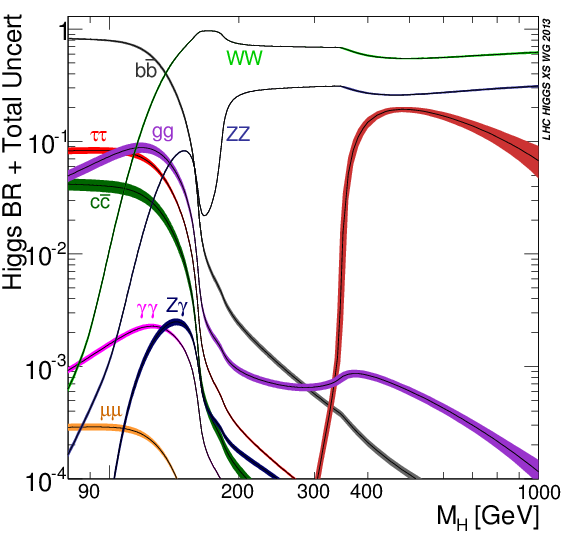
\includegraphics[width=3in]{images/Higgs_BR.png}
  \begin{tabular}{ |l|l| }
    \hline
    \multicolumn{2}{|c|}{Higgs Branching Ratios} \\
    \hline
    ${\rm b\bar{b}}$ & 0.57 \\
    WW & 0.22\\
    gg & 0.085 \\
    ${\rm \tau\tau}$ & 0.065 \\
    ZZ & 0.027 \\
    ${\rm c\bar{c}}$ & 0.027 \\
    ${\rm \gamma\gamma}$ & 0.0023 \\
    ${\rm Z}\gamma$ & 0.0016 \\
    ${\rm \mu^{+}\mu^{-}}$ & 0.00022 \\
    \hline
  \end{tabular} 
  \caption
{The graphic on the top left presents the SM Higgs branching fractions as functions of mass while the table on the bottom right displays the branching fractions for a 125 GeV SM Higgs \cite{crossbranchplots}.}
  \label{fig:hbranch}
\end{figure}

The muon has the lowest mass -- excluding the photon and gluon -- of the particles in Figure ~\ref{fig:hbranch} and consequently H$\rightarrow \mu^{+}\mu^{-}$ has the lowest branching fraction in the set. \footnote{The Higgs also couples to the electron and the first generation quarks but the masses are so light that CMS does not expect to see the SM Higgs in those modes.} The gluons and photons are massless and do not couple to the Higgs at leading order. These massless vector bosons interact with the Higgs through a loop of top quarks. The extremely heavy mass of the top quark, about 173 GeV, balances the fact that the loop production is a higher order mechanism.  
\begin{figure}[h!]
  \centering
  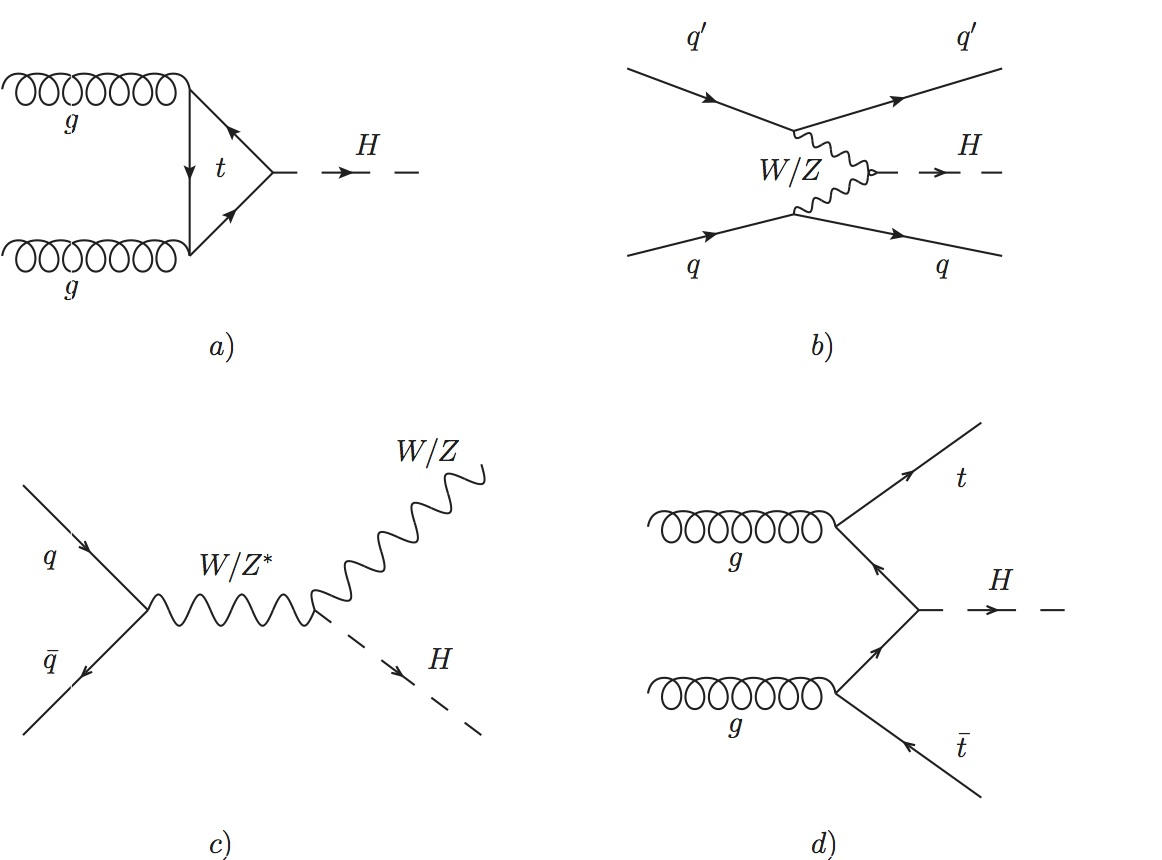
\includegraphics[width=4in]{images/higgs_production_modes.png}
  \caption
   {The SM production modes with the highest cross sections. a) Gluon Gluon Fusion (GF) b) Vector Boson Fusion (VBF) c) Associated Production with a Vector Boson (VH) d) ${\rm t\bar{t}}$H}
  \label{fig:hfeynprod}
\end{figure}

The Higgs to massless vector boson coupling via the top loop is seen in the GF Feynman diagram in Figure ~\ref{fig:hfeynprod}. At ${\rm M_{h} = 125}$ GeV, ${\rm \sqrt{s} =}$ 13 TeV, the GF channel comprises 87\% of the total Higgs production cross section, VBF 7\%, VH 4\%, and ${\rm t\bar{t}}$H 1\% \cite{crossbranchplots}. Besides ${\rm t\bar{t}}$H, the process q + $\bar{q} \rightarrow$ H isn't considered due to its low cross section. The low masses of the other quarks suppress the process. 

Quark gluon (qg) scattering is a major background for the Higgs to two jets decays since the process closely resembles GF in this mode.   

\begin{figure}[h!]
  \centering
  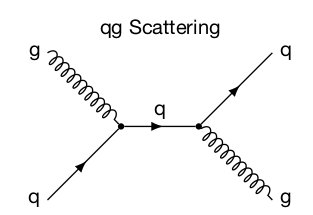
\includegraphics[width=2in]{images/qg_scattering.png}
  \caption
   {Quark gluon scattering creates many two jet events. This background looks very similar to GF when the Higgs decays to two jets. The colliding protons are made of quarks and gluons so this process is extremely common.}
  \label{fig:feynqg}
\end{figure}


\chapter{DISCOVERY, LIMITS, MEASUREMENT, AND SENSITIVITY} \label{coinflip}

This chapter briefly covers the statistical methods needed for the $H\rightarrow\mu^+\mu^-$ search. The test of a coin for bias is used as a simple example to explain the concepts of discovery, limits, measurement and sensitivity. These concepts are then extended to a binned counting experiment typical in particle physics. The chapter starts with discovery. 

\section{Discovery}
Proof by contradiction may be used as a framework for discovery. If there are only two logical possibilities either A or B, then if A is ruled out, B must be true. The hypothesis to disprove (A) in order to claim B is called the null hypothesis. By disproving a null hypothesis like "the effect X does not exist" a scientist may claim the discovery of X. For example, to test whether a coin is biased, the experimenter assumes the null hypothesis that the coin is unbiased and then performs an experiment, tossing the coin many times. If all of the tosses are heads, then it's very unlikely that the coin is unbiased, and it's therefore reasonable to rule out the null and to declare the discovery of a biased coin. 

In order to quantify how rarely an unbiased coin would yield an experiment with $N_{heads}$, a model for the probability density function (PDF) is needed. The binomial distribution with $x = N_{heads}$, $\rho = p_{heads} = 0.5$, and $N = N_{tosses}$, is the appropriate PDF,
\begin{equation}
p(x,N;\rho) = \frac{N!}{x! (N - x)!}\rho^{x}(1-\rho)^{N-x}.
\end{equation}
With the PDF, the probability for the null to produce different experiments can be compared in terms of p-values. The p-value assuming the null, $P(x \succ Y|null)$, is the probability to observe something at least as extreme, $\succ$, as the outcome Y given the null. Declaring the cutoff p-value for the coin flipping experiment sets the minimum threshold of heads, $h_{cutoff}$, needed for discovery. Any observation of $x=N_{heads}$ with a p-value rarer than the cutoff, i.e. $P(x \geq h_{cutoff}|null) < p_{cutoff}$, will rule out the null hypothesis. 

Traditionally, different fields require different p-values, and in high energy physics 3$\sigma$ leads to an "observation" and 5$\sigma$ leads to a "discovery". These correspond to p-values of 0.3\% and 0.00006\% respectively. 
\begin{figure}[h!]
  \centering
  \includegraphics[width=3in]{images/stat/p-value.png}
  \caption[An illustrated example of a p-value.]
   {The shaded region represents the p-value for an observation of $N_{heads}=h$. If the p-value for h is lower than the cutoff threshold, then the null hypothesis can be ruled out and a discovery may be declared.}
\label{fig:pvalue_ex}
\end{figure}
As an example, observing 65 heads or greater in 100 tosses occurs just less than 0.3\% of the time for an unbiased coin. Therefore, any experiment with $N_{heads} \geq 65$ would invalidate the null at $3\sigma$ and lead to an observation of bias.

\section{Limits}

Besides discovery, setting a limit is also important. Upon tossing a coin 100 times and finding $N_{heads}=40$, the experimenter may ask which values of $p_{heads}$ are too high to yield such a low observation. In this case, all values of $p_{heads}$ that predict experiments with 40 heads or fewer at too rare a probability may be ruled out at some confidence. For 95\% confidence, $p_{heads} \geq 0.488$ may be ruled out as $p_{heads} \geq 0.488$ yields 40 heads or fewer less than $5\%$ of the time, while smaller values for $p_{heads}$ do not. Therefore, observing 40 heads in 100 tosses places an upper limit of $p_{heads}=0.488$ on the bias of the coin at 95\% confidence. 

\section{Measurement and Uncertainty}
\label{meas}
 
Finally, measuring values is also important. In the case of the coin, the experimenter flips the coin 100 times and attempts to measure how biased the coin is. The value stated as the measured value is usually the best fit, and the best fit value is the one that maximizes the (log) likelihood of seeing the data observed. In practice, minimizing the \textit{negative log likelihood} ($N_{LL}$) is more convenient, 
\begin{equation}
-\frac{\partial}{\partial \rho}ln\left(p(x,N;\rho)\right) = 0 \rightarrow \hat{\rho} = \frac{x}{N}.
\end{equation}   
When performing many independent experiments the PDFs for each experiment multiply and the negative log likelihood is,
\begin{equation}
-ln(p) = -ln\left(\prod_i p_i\right) = -\sum_i ln\left(p_i\right).
\end{equation}
Over many coin flipping experiments, the best fit value for $\rho$ is
\begin{equation}
-\frac{\partial}{\partial \rho}ln(p) = 0 \rightarrow \hat{\rho} = \frac{\sum_{i=1}^{n} x_i}{\sum_{i=1}^{n} N_i}.
\end{equation}
When $N_i$ is the same in each experiment the best fit is just the mean over all experiments,
\begin{equation}
\hat{\rho} = \frac{1}{n} \sum_{i=1}^{n} \frac{x_i}{N} = \frac{1}{n} \sum_{i=1}^{n} \hat{\rho}_i.
\end{equation}
Note that the different experiments all contribute to determine the best fit, and that the results of other experiments constrain the influence of a particular experiment to declare the best fit value.  

In order to quantify the uncertainty of the measured value, limiting values of $\rho$ are computed. The upper limit $\rho_{hi}$ and the lower limit $\rho_{lo}$ define the confidence interval $[\rho_{lo}, \rho_{hi}]$, which quantifies the uncertainty on $\hat{\rho}$. Conceptually, the interval is a range of values for which the observed data (summarized by $\hat{\rho}$) is not too extreme. The confidence interval stated usually corresponds to $1\sigma$ or 68\%, constructed from upper and lower limits that exclude 16\% of their respective PDFs. The construction is illustrated in Figure \ref{fig:meas_uncertainty}, and the construction guarantees that in many experiments the true value will be contained in the confidence interval 68\% of the time.    

\begin{figure}[h!]
  \centering
  \includegraphics[width=6in]{images/stat/plow_and_phi.png}
  \caption[Defining the confidence interval.]
   {The $1\sigma$ uncertainty on $\hat{\rho}$ is determined by finding the appropriate $\rho_{lo}$ and $\rho_{hi}$. $\rho_{lo}$ is the value of $\rho$ just low enough that an observation corresponding to $\hat{\rho}$ or greater occurs only 16\% of the time. $\rho_{hi}$ is the value of $\rho$ just high enough that an observation of $\hat{\rho}$ or less occurs only 16\% of the time. The shaded region represents 16\% of the respective PDF.}
\label{fig:meas_uncertainty}
\end{figure}

Observing 50 heads in 100 tosses leads to $\hat{\rho} = 0.5$ and a corresponding $1\sigma$ confidence interval of $[0.44, 0.56]$. The measurement is then reported as $\hat{\rho} = 0.5^{+0.6}_{-0.6}$. An experiment with more data generally has a lower uncertainty on the measured value. For example, observing 450 heads in 900 tosses leads to $\hat{\rho} = 0.5^{+0.2}_{-0.2}$. Note that the uncertainty shrinks with $\sqrt{N_{tosses}}$, $\frac{0.6}{0.2} = 3 = \sqrt{\frac{900}{100}}$.

Sometimes the limits in the uncertainty calculation are circumvented by assuming that the likelihood becomes Gaussian with enough statistics. When the likelihood is a Gaussian, the interval is simply $\hat{\mu} \pm \sigma$. The negative log likelihood in the Gaussian case is
\begin{equation}
N_{LL} = -ln[p] = -ln\left[Ae^{\frac{(x-\mu)^2}{2\sigma^2}}\right]= -ln[A] + \frac{(x-\mu)^2}{2\sigma^2}.
\end{equation}
Expanding about the minimum, $\hat{\mu}$, provides an estimate of $\sigma$ and hence the confidence interval, 
\begin{equation}
N_{LL}(\hat{\mu}) + 0(x-\hat{\mu}) + \frac{1}{2}N_{LL}''(\hat{\mu})(x-\hat{\mu})^2 = -ln[A] + \frac{(x-\hat{\mu})^2}{2\sigma^2} \rightarrow \sigma^2 = \frac{1}{N_{LL}''(\hat{\mu})}.
\end{equation}
Note that $\sigma$ may be determined by moving x away from the minimum until $\Delta N_{LL} = 1$. The $\Delta N_{LL} = 1$ method is sometimes used as an estimate of the uncertainty even when the likelihood is not Gaussian. In some cases the PDF may be multidimensional, and in those cases, $\sigma^2$ is the covariance matrix with $\partial_{\theta_i}\partial_{\theta_j}N_{LL}(\hat{\theta}) = (\sigma^2)^{-1}_{ij}$. Multidimensional or otherwise, $\sigma$ can be used to estimate the uncertainty on the best fit values. 

\section{Sensitivity}

An analysis is often designed to maximize the chance of discovery by minimizing the expected p-value. The lower the expected p-value given the null, the higher the sensitivity. This section uses a limiting case of the binomial distribution to point out the factors that contribute to a sensitive analysis. Consider an experiment flipping a coin N times, 
\begin{equation}
p(x,N;\rho) = \frac{N!}{x! (N - x)!}\rho^{x}(1-\rho)^{N-x}.
\end{equation}
The experimenter may ask what p-value is expected if the coin has a true value $\rho=\rho_i$. For a coin with $\rho_i$, the observed $N_{heads}$ is most frequently $N\rho_i$. Therefore, given the null with $\rho=\rho_{null}$ one expects
\begin{equation}
p(x=N\rho_i,N;\rho=\rho_{null}) = \frac{N!}{(N\rho_i)! (N - N\rho_i)!}\rho_{null}^{N\rho_i}(1-\rho_{null})^{N-\rho_i}.
\end{equation}
When $N\rho$ is far enough from zero, the binomial distribution may be approximated by a Gaussian with mean $\mu=N\rho$, and standard deviation $\sigma=\sqrt{N\rho(1-\rho)}$. In this limit, the relationship between the expected p-value and the hypotheses are easy to see, because the p-values for a Gaussian are determined by the number of standard deviations away from the mean, Z. The sensitivity is given by $Z=\frac{(x-\mu)}{\sigma}$, and for a coin with $\rho_i$, the expected sensitivity is 
\begin{equation}
Z = \frac{(x-\mu)}{\sigma} = \frac{N(\rho_i - \rho_{null})}{\sqrt{N\rho_{null}(1-\rho_{null})}} = \frac{\sqrt{N}(\rho_i - \rho_{null})}{\sqrt{\rho_{null}(1-\rho_{null})}}.
\end{equation}
The larger Z is, the smaller the p-value, and the more sensitive the experiment. Note that the sensitivity scales as the $\sqrt{N}$, which shows that collecting more data improves the sensitivity to discovery. 

\section{Constraints And Nuisance Parameters}
\label{constraints}

As alluded to in Section \ref{meas}, additional measurements provide constraints on the parameters of a PDF. Consider two experiments tossing the same coin with y heads observed in the first experiment and x in the second. In this case, the likelihoods of the individual experiments are multiplied to determine the net likelihood, 
\begin{equation}
p(x, y; \rho) = p(x; \rho)p(y; \rho),
\end{equation}
Upon minimizing the negative log-likelihood, the observations of the first experiment fight with the second experiment to determine the best fit for $\rho$. 

Sometimes it is convenient to replace the actual likelihood of the previous experiment with a suitable representative. Often, a Gaussian is used along with the best fit and the uncertainty of the previous experiment, $\hat{\rho}_{y}$ and $\sigma_y$. The net likelihood then becomes,
\begin{equation}
p(x; \rho) = p(x; \rho) \mathcal{N}(\hat{\rho}_y; \mu=\rho, \sigma=\sigma_y).
\end{equation}
The Gaussian ($\mathcal{N}$) fights to keep $\hat{\rho}$ near $\hat{\rho}_y$ with a strength dependent on $\sigma_y$. Other constraints like the log-normal or Poisson distributions are also used. Constraint terms are especially useful when they replace a complicated likelihood with many data points. 

Imagine a case where the distribution of dirt on a coin affects the net bias $\rho$. The fraction of heads expected then depends on the bias of the coin itself and the additional bias from the dirt, $\rho = \rho_{coin} + \rho_{dirt}$. If a complicated measurement is made to determine the distribution of dirt on the coin, thus estimating $\rho_{dirt}$, then the bias of the coin itself $\rho_{coin}$ can be extracted. The net likelihood includes the likelihood for the set of observations y
\begin{equation}
p(x, y; \rho_{coin}, \rho_{dirt}) = p(x; \rho_{coin}, \rho_{dirt})p(y; \rho_{dirt}).
\end{equation}

The observations y determine the best fit $\hat{\rho}_{y-dirt}$ and uncertainty $\sigma_{y-dirt}$ from that experiment, and the likelihood becomes, 
\begin{equation}
p(x, \hat{\rho}_{y-dirt}; \rho_{coin}, \rho_{dirt}) = p(x; \rho_{coin}, \rho_{dirt})
                                   \mathcal{N}(\hat{\rho}_{y-dirt}; \mu=\rho_{dirt}, \sigma=\sigma_{y-dirt}),
\end{equation}
where a Gaussian constraint replaces the complicated likelihood of the $\rho_{dirt}$ measurement involving the data points y. The best fit for $\rho_{coin}$ can be calculated using the maximum likelihood estimates for $\rho_{coin}$ and $\rho_{dirt}$ given x and $\hat{\rho}_{y-dirt}$. Limits and uncertainty on $\rho_{coin}$ can be calculated by \textit{profiling} the likelihood,  
\begin{equation}
p(x, \hat{\rho}_{y-dirt}; \rho_{coin}, \hat{\hat{\rho}}_{dirt}) = p(x; \rho_{coin}, \hat{\hat{\rho}}_{dirt})
                                   \mathcal{N}(\hat{\rho}_{y-dirt}; \mu=\hat{\hat{\rho}}_{dirt}, \sigma=\sigma_{y-dirt}).
\end{equation}
The double hat designates a maximum likelihood estimate of the parameter for fixed $\rho_{coin}$. The parameters other than the parameter of interest are called \textit{nuisance parameters}, and profiling sets the nuisance parameters to their best fit estimates for some fixed value of the parameter of interest. 

The distribution for $p(x, \hat{\rho}_{y-dirt}; \rho_{coin}, \hat{\hat{\rho}}_{dirt})$ can be simulated using Monte Carlo methods, where $\hat{\rho}_{y-dirt}$ is a random variable drawn from $\mathcal{N}(\hat{\rho}_{y-dirt}; \mu=\hat{\hat{\rho}}_{dirt}, \sigma=\sigma_{y-dirt})$. The randomness of $\hat{\rho}_{y-dirt}$ smears the distribution for $\hat{\rho}_{coin}$ and widens its uncertainty. The uncertainty of $\hat{\rho}_{y-dirt}$ also leads to looser the limits on $\rho_{coin}$.

\section{A Particle Physics Search}

This section extends the previous concepts to the search for a new particle in high energy particle physics. Such a search makes use of two hypotheses: the background only (B) and the signal plus background (S+B). The background only predicts the number of events if the particle does not exist, and the signal plus background (S+B) predicts the number of events if the particle does exist. The signal (S) represents the number of additional events expected if the new particle exists.

\begin{figure}[h!]
  \centering
  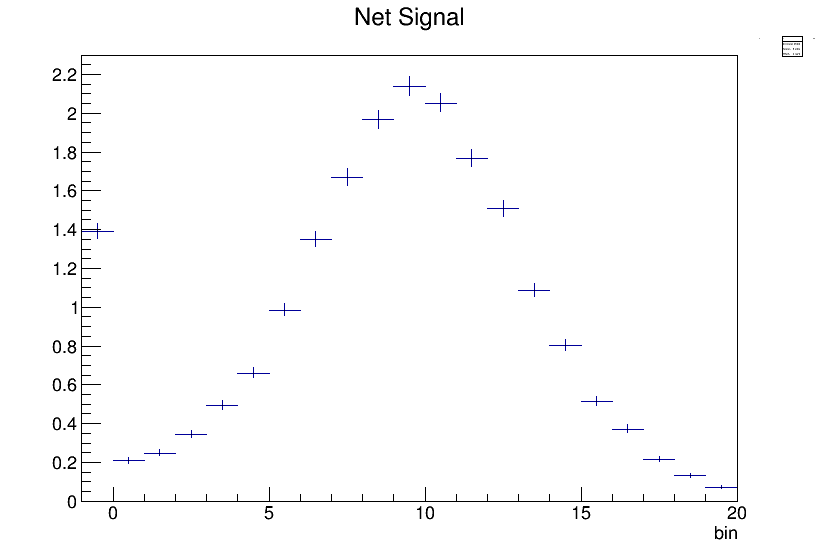
\includegraphics[width=0.49\linewidth]{images/bdt_cats/binning_signal_example.png}
  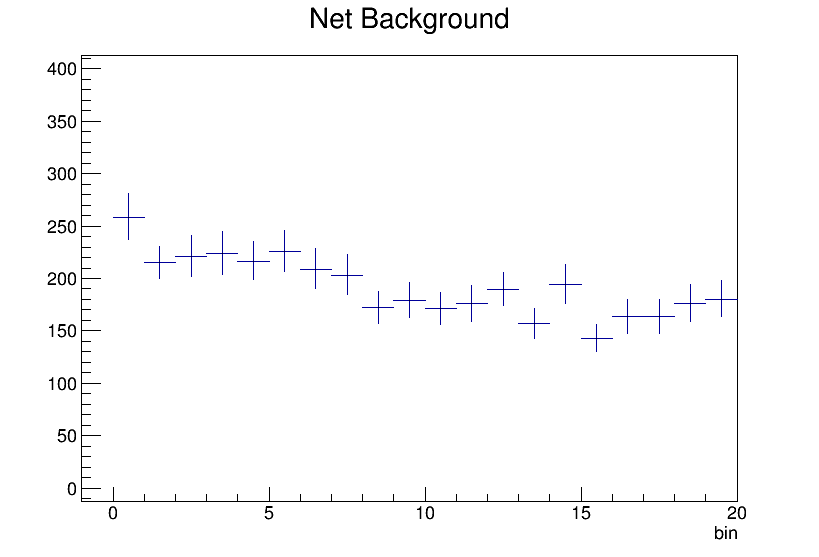
\includegraphics[width=0.49\linewidth]{images/bdt_cats/binning_bg_example.png}
  \caption[An example of the signal and background used for the background only and S+B hypotheses.]
  {An example of the binned signal and background used for the background only and S+B hypotheses.}
  \label{fig:sb_binning_example}
\end{figure}

The S+B and B hypotheses are usually one dimensional distributions binned along some variable. If the observed distribution of events is too different from the background only, the background only hypothesis is ruled out and the experiment proclaims the discovery of a new particle. The distribution describing the amount of signal (S) is often reported in terms of the signal strength ($\nu$) \footnote{Usually $\mu$ denotes the signal strength, but $\mu$ was already used in this section to designate the Gaussian mean.} and the SM prediction (s) allowing the signal hypothesis to be written $S = \nu s$. A signal strength of 1 means that the signal model S is simply the Standard Model prediction, and a signal strength of 2 means that S has twice the signal as the SM prediction in each bin.  

The probability to observe a particular count in a bin is described by the Poisson distribution
\begin{equation}
p\left( x; \lambda \right) = \frac{{e^{ - \lambda } \lambda^x }}{{x!}},
\end{equation}
where $\lambda$ is the expected number of events and x is the observed number of events. A valid hypothesis provides the expected number of events in each bin and the data provides the observed number in each bin. The expected number of events in a bin is given by $\lambda$ and the standard deviation is $\sigma = \sqrt{\lambda}$. When $\lambda$ is far enough from zero the Poisson distribution may be described by a Gaussian with mean $\mu = \lambda$ and standard deviation $\sigma = \sqrt{\lambda}$.  

\subsection{Sensitivity}
\label{sensitivity}

The sensitivity becomes much more interesting with binned distributions. First consider the sensitivity for a single bin. If the Standard Model or some other theory predicts the expected number of events in a bin to be $\lambda_i=S_i+B_i$ and the null predicts $\lambda_i=B_i$, then the expected sensitivity for discovery is,
\begin{equation}
Z = \frac{(x_i-\mu_i)}{\sigma_i} = \frac{(S_i+B_i-B_i)}{\sqrt{B_i}} = \frac{S_i}{\sqrt{B_i}} = \frac{\sqrt{N}\rho_{si}}{\sqrt{\rho_{bi}}}.
\end{equation}
As before, this scales with the $\sqrt{N}$. So, again, one way to ensure a sensitive experiment is to collect a lot of data, but that's not the only way. With many bins, the PDFs for each bin multiply and the $N_{LL}$ in the Gaussian limit is,
\begin{equation}
\label{eq:norm}
-ln\left(\frac{p}{C}\right) = -ln\left(\prod_i p_i\right) + ln\left( C \right) 
                            = -\sum_i ln\left(p_i\right) + ln\left( C \right) 
                            = \sum_i \frac{(x_i-\mu_i)^2}{2\sigma_i^2},
\end{equation}
where C is the sum of the normalizations for the Gaussians. After normalizing by C and the factor of 2, the $N_{LL}$ is a sum of $\chi^2$ variables and is therefore itself a $\chi^2$ variable, 
\begin{equation}
\chi^2_{nll} = -2ln\left(\frac{p}{C}\right) = \sum \frac{(x_i-\mu_i)^2}{\sigma_i^2}.
\end{equation}
This shows that the expected sensitivity with many Poissonian bins may be estimated by
\begin{equation}
Z^2 = \frac{(x_{nll}-\mu_{nll})^2}{\sigma_{nll}^2} = \sum_i \frac{S_i^2}{B_i}.  
\end{equation}
By concentrating the fixed amount of signal into a few bins with low background the sensitivity may improve regardless of the data available. This is indicative of the idea that the null may be invalidated when the data observed is many times the expected fluctuations.

\subsection{Test Statistic}

The negative log likelihood can be used to form the test statistic t, a random variable that summarizes the total discrepancy between the observed data and a given theory. The statistic is nice because it reduces the multitude of discrepancies in the many bins to a single number. The test statistic t is given by, 
\begin{equation}
t = -2ln\left(\frac{p(x_i,\theta)}{p(x_i,\hat{\theta})}\right).
\end{equation}
The normalization, $p(x_i,\hat{\theta})$, is the PDF with the parameters set to the best fit values, and this term as in Equation \ref{eq:norm} sets the range of t from zero to infinity. When there is only one parameter of interest $\nu$ the likelihood may be reduced to one dimension by profiling the nuisance parameters $\theta$,
\begin{equation}
t = -2ln\left(\frac{p(x_i,\nu,\hat{\hat{\theta}})}{p(x_i,\hat{\theta})}\right).
\end{equation}
As before, the $\hat{\hat{\theta}}$ parameters are the best fit values for a fixed parameter of interest $\nu$. The profiled test statistic may be used to set limits on the parameter of interest. Asymptotically, the test statistic is a $\chi^2$ variable. See the analysis of Section \ref{sensitivity}. Constraints may be included as necessary. 

\subsection{Constraints}

When previous fits have been performed to determine certain parameters and their uncertainty, the likelihoods can be included to encode the information. The measurements on the nuisance parameters $\theta$ are included like so,
\begin{equation}
p(x_i; \nu, \theta) = \prod_i Poisson(x_i, \lambda_i(\nu, \theta))\prod_j p(y_j, \theta_j),
\end{equation}
where $y_j$ represents the previously observed data and $\nu$ represents the signal strength. As in Section \ref{constraints}, the observations $y_j$ are summarized by the best fits ($\bar{\theta_j}$) rather than keeping track of the actual data. The net likelihood becomes,
\begin{equation}
p(x_i; \nu, \theta) = \prod_i Poisson(x_i; \lambda_i(\nu, \theta))\prod_j C(\bar{\theta_j}, \theta_j, \sigma_j),
\end{equation}
where C designates some constraint PDF. Constraints implement the various systematic and theoretical uncertainties involved in the analysis.  

\subsection{Using The Test Statistic}

With a model for the expected yields in each bin, the distribution for t may be approximated by Monte Carlo methods, or by assuming that with enough data t reduces to a $\chi^2$ distribution. The expected p-value against the background only may be calculated using the expected yields for S+B as the expected hypothesis and the background only yields as the null. Similarly, the expected upper limit on S may be calculated using t with S+B as the null and the background as the expected hypothesis. The expected upper limit at 95\% confidence is calculated by finding the value of S high enough that observing the expected background-only has a p-value of 5\%. A higher expected sensitivity and lower expected upper limit are important goals in the design of a physics analysis.

Upon collecting data, the test statistic t may be used with the data observed and the background only as the null to check for discovery. The observed upper limit on S at 95\% confidence is computed by finding a high enough value of S such that observing the data has a p-value of $5\%$. These can be compared to the expected p-value and the expected upper limit. 
 
In high energy physics the CLs method is often used to set the upper limits. The CLs method reports an upper limit using an adjusted p-value, $p_{CLs} = \frac{p_\mu}{p_{bkg-only}}$, where $p_{\mu}$ is the probability for a theory with a true parameter $\mu$ to observe x or less data and $p_{bkg-only}$ is the probability for the background only to observe x or less data. Using the CLs method at 95\% confidence, $p_\mu$ must be $0.05p_{bkg-only}$ or less. When the data observed is much greater than the median expected background, the integrated probability less than the observed is most of the distribution, $p_{bkg-only}$ goes to 1, and the CLs upper limit approaches the standard upper limit. But in general, $p_{bkg-only}$ is less than one yielding a $p_{CLs}$ greater than $p_\mu$ and a CLs limit that is more conservative than the standard upper limit. The CLs construction guarantees that hypotheses with low $p_{\mu}$ must also differ substantially from the background to be ruled out.   


%%%%%%%%%%%%%%%%%%%%%%%%%%%%%%% SOME SAVED INFO ON LIMITING CASE FOR UNCERTAINTY %%%%%%%%%%%%%%%%%%%%%%%%


\chapter{THE $H\rightarrow\mu^+\mu^-$ SEARCH STRATEGY} \label{strategy}

The goal of the $H\rightarrow\mu^+\mu^-$ search is to discover the decay, and barring that to set an upper limit on the rate of production. The best fit for the rate of production is also reported. In order to do all of this, the analysis needs the data along with the expected yields for the signal and background. The expected yields determine the likelihood, the PDF for the test statistic t, and the limits/p-values. The analysis fits Monte Carlo samples along $m_{\mu^+\mu^-}$ for the signal and fits data along $m_{\mu^+\mu^-}$ for the background. The data at the collected luminosity has far better statistics than the Monte Carlo available for the background, and the larger statistics provide lower uncertainty in the bins of the PDF. The data and MC samples used in the analysis are covered in Chapter \ref{samples}, and the models for the signal and background are covered in Chapter \ref{modeling}. 

There is too much data to process to use all of it in the statistical analysis, and that would be wasteful anyways, so basic selections are made to look only at data likely to contain $H\rightarrow\mu^+\mu^-$ signal and unlikely to miss it. With a reasonable amount of data to look at, the Monte Carlo is validated against the data to make sure it agrees with observation. Some corrections like efficiency scale factors, trigger scale factors, and momentum corrections are applied to the Monte Carlo to ensure better agreement with the data. The background Monte Carlo is used to help with the data Monte Carlo validation, and to optimize the sensitivity, but not for the limit setting, discovery p-values, or measurement. The event seletion and corrections are also covered in Chapter \ref{samples}. 

The analysis attempts to maximize the odds of discovering $H\rightarrow\mu^+\mu^-$ by maximizing the sensitivity. Because the sensitivity increases with the amount of data, improvements to the Level-1 Muon Trigger are made to increase the $\mu^+\mu^-$ data saved for the analysis. Moreover, the sensitivity improves with increased signal and worsens with increased background -- recall that in the limit of large statistics, $Z^2=\sum_i\frac{S_i^2}{B_i}$. As such, the ideal situation is one where the signal is concentrated into a single bin with little or no background. This isn't possible in practice, but regions of feature space may be found where the signal is more concentrated or where there is little background or both. 

The analysis corrects the muon momentum to narrow the $m_{\mu^+\mu^-}$ peak, improving its resolution, concentrating the signal, and improving the data/MC agreement. To further improve the sensitivity, Boosted Decision Trees (BDTs) \cite{bdt} are trained to separate signal and background. The training produces a discriminating feature with a higher conentration of signal and lower concentration of background at large values. A novel algorithm then optimally and automatically categorizes the events by resolution and BDT score to maximize the expected sensitivity of the analysis. When the S+B fit is along a single dimension like $m_{\mu\mu}$, low sensitivity regions merge with high sensitivity regions of feature space polluting the chance for discovery. The categorization extracts the high sensitivity regions to regain the sensitivity. 

The muon momentum corrections are covered in Chapter \ref{samples}. The work to optimize the sensitivity is covered in Chapter \ref{optimize}. The limits, p-values, and signal strength measurement are presented in Chapter \ref{results}.


\chapter{SAMPLES, CORRECTIONS, AND SELECTIONS FOR THE $H\rightarrow\mu^+\mu^-$ SEARCH} \label{samples}

This chapter presents the data and MC samples used in the analysis, the corrections to improve the data/MC agreement, and the selections defining the events used.

%%%%%%%%%%%%%%%%%%%%%%%%%%%%%%%%%%%%%%%%%%%%%%%%%%%%%%%
\section{Data And Monte Carlo Samples} \label{sampsec}

The proton-proton collision data used for the $H\rightarrow\mu^+\mu^-$ search is listed in Table \ref{tab:data}. The signal processes in \ref{fig:hfeynprod2} are represented by the MC in Table \ref{tab:sigmc}. The signal PDF is formed by fitting the GGF, VBF, W$^+$H, W$^-$H, ZH, and ttH MC then adding the fits together. The background MC used to optimize the categorization and to validate the simulation is listed in Table \ref{tab:bkgmc}. While the background MC is used for validation and optimization, the background PDF used in the limit setting is formed by fitting the data in signal free control regions. 

\begin{figure}[h!]
  \centering
  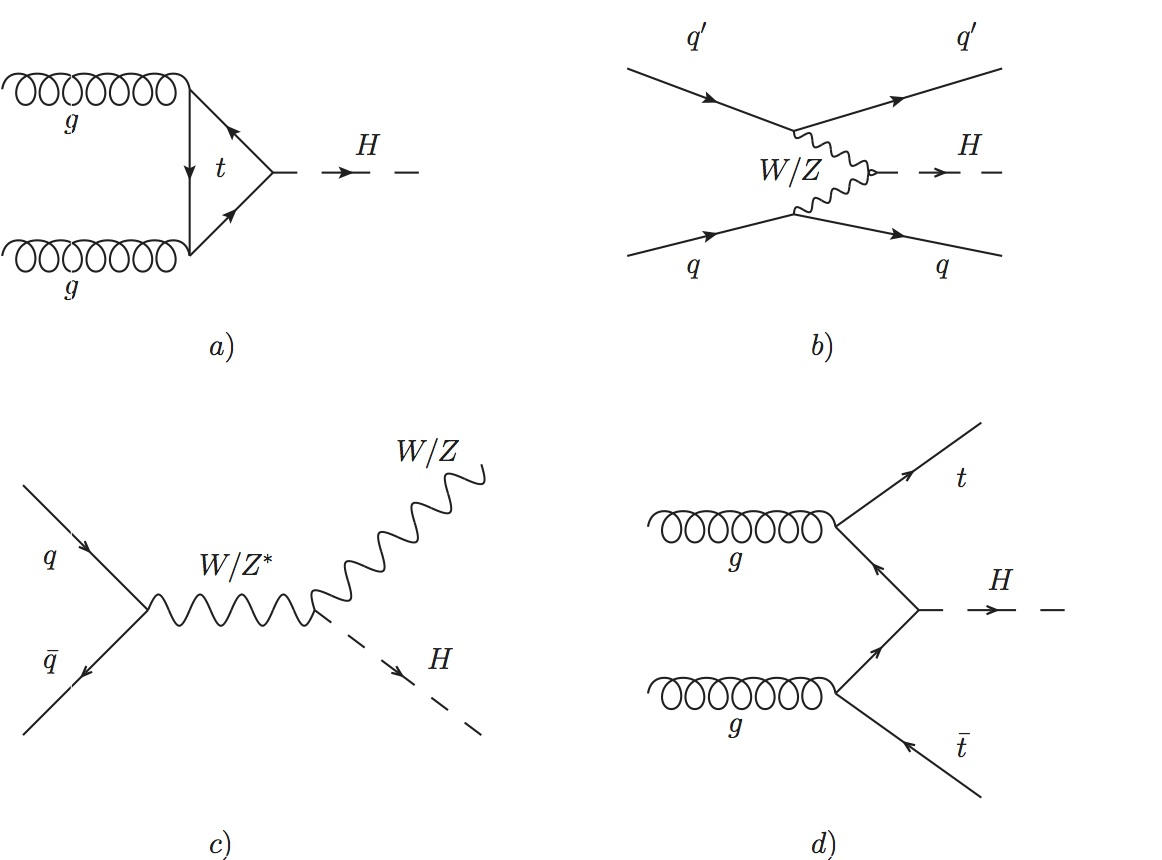
\includegraphics[width=4in]{images/higgs_production_modes.png}
  \caption[Standard Model Higgs boson production modes.]
   {The SM production modes considered in the analysis. a) Gluon Gluon Fusion (GGF) b) Vector Boson Fusion (VBF) c) Associated Production with a Vector Boson (VH) d) Associated production with top quarks ${\rm t\bar{t}}$H}
  \label{fig:hfeynprod2}
\end{figure}

\begin{table}[!h]
\label{tab:data}
\caption{Overview of the single muon data stream collected during the proton-proton collisions at $\sqrt{s}=13$~TeV by CMS at the LHC in 2016.}
\small
\renewcommand{\arraystretch}{1.5}

\begin{tabular}{llc}
        \hline 
        Dataset & Run Range & Integrated Luminosity [fb$^{-1}$]\\
        \hline
        \url{/SingleMuon/Run2016B-03Feb2017_ver2-v2/MINIAOD} & 272007-275376 & 5.788 \\
        \url{/SingleMuon/Run2016C-03Feb2017-v1/MINIAOD}      & 275657-276283 & 2.573 \\
        \url{/SingleMuon/Run2016D-03Feb2017-v1/MINIAOD}      & 276315-276811 & 4.248 \\
        \url{/SingleMuon/Run2016E-03Feb2017-v1/MINIAOD}      & 276831-277420 & 4.009 \\
        \url{/SingleMuon/Run2016F-03Feb2017-v1/MINIAOD}      & 277772-278808 & 3.102 \\
        \url{/SingleMuon/Run2016G-03Feb2017-v1/MINIAOD}      & 278820-280385 & 7.540 \\
        \url{/SingleMuon/Run2016H-03Feb2017_ver2-v1/MINIAOD} & \multirow{2}{*}{280919-284044} & \multirow{2}{*}{8.606} \\ 
        \url{/SingleMuon/Run2016H-03Feb2017_ver3-v1/MINIAOD} &                                &                        \\
        \url{/SingleMuon/Run2016*-03Feb2017-v*/MINIAOD}      & 272007-280385 & 35.866 \\
                                                                %% Adds up to 35.866 - i.e. 35.9 fb^-1
        \hline
        \multicolumn{3}{l}{Luminosity mask: \url{Cert_271036-284044_13TeV_23Sep2016ReReco_Collisions16_JSON.txt}}    \\
\end{tabular}
\end{table}

\newpage
\begin{landscape}
\begin{table}[p]
\label{tab:sigmc}
\caption{The Higgs signal MC samples were generated with {\sc POWHEG}
while the parton shower and hadronization processes are modeled by the
{\sc Pythia8} generator with TuneCUETP8M1.}
\renewcommand{\arraystretch}{1.5}
\tiny
\begin{tabular}{lccc}
  \hline
  Higgs signal MC samples & Events & Cross section [pb] & Xsec $\times$ BR [fb]  \\
  \hline
  \url{/GluGlu_HToMuMu_M125_13TeV_powheg_pythia8/RunIISummer16MiniAODv2-PUMoriond17_80X_mcRun2_asymptotic_2016_TrancheIV_v6-v1/MINIAODSIM }  &  250000 & 48.58    & 10.571   \\
  \url{/VBF_HToMuMu_M125_13TeV_powheg_pythia8/RunIISummer16MiniAODv2-PUMoriond17_80X_mcRun2_asymptotic_2016_TrancheIV_v6-v1/MINIAODSIM }     &  249200 &  3.7817  & 0.8229   \\
  \url{/WPlusH_HToMuMu_M125_13TeV_powheg_pythia8/RunIISummer16MiniAODv2-PUMoriond17_80X_mcRun2_asymptotic_2016_TrancheIV_v6-v1/MINIAODSIM }  &  124547 &  0.09426 & 0.02051  \\
  \url{/WMinusH_HToMuMu_M125_13TeV_powheg_pythia8/RunIISummer16MiniAODv2-PUMoriond17_80X_mcRun2_asymptotic_2016_TrancheIV_v6-v1/MINIAODSIM } &  125000 &  0.05983 & 0.013019 \\
  \url{/ZH_HToMuMu_M125_13TeV_powheg_pythia8/RunIISummer16MiniAODv2-PUMoriond17_80X_mcRun2_asymptotic_2016_TrancheIV_v6-v1/MINIAODSIM }      &  249748 &  0.17762 & 0.03865  \\
\hline
\end{tabular}

\end{table}
\end{landscape}

\newpage
\begin{landscape}
\begin{table}[p]
\label{tab:bkgmc}
\caption{The background MC samples were generated with {amc@NLO}.
{\sc POWHEG} and {\sc madgraph}. Spin effects in multi-boson processes are
simulated using {\sc madspin}. The parton shower and hadronization processes
are modeled by the {\sc Pythia8} generator with TuneCUETP8M1.}
\tiny
\renewcommand{\arraystretch}{1.2}
\begin{tabular}{lcc}
        \hline 
        Background MC & Events & Cross Section [pb]  \\
        \hline
        \multicolumn{3}{c}{Drell--Yan}  \\
        \url{/DYJetsToLL_M-50_TuneCUETP8M1_13TeV-amcatnloFXFX-pythia8/RunIISummer16MiniAODv2-PUMoriond17_80X_mcRun2_asymptotic_2016_TrancheIV_v6_ext2-v1/MINIAODSIM} &  122055388 & 5765  \\
        \url{/DYToLL_0J_13TeV-amcatnloFXFX-pythia8/RunIISummer16MiniAODv2-PUMoriond17_80X_mcRun2_asymptotic_2016_TrancheIV_v6_ext1-v1/MINIAODSIM} & 49579613  &  4754\\
        \url{/DYToLL_1J_13TeV-amcatnloFXFX-pythia8/RunIISummer16MiniAODv2-PUMoriond17_80X_mcRun2_asymptotic_2016_TrancheIV_v6_ext1-v1/MINIAODSIM} & 49902571  & 888.9 \\
        \url{/DYToLL_2J_13TeV-amcatnloFXFX-pythia8/RunIISummer16MiniAODv2-PUMoriond17_80X_mcRun2_asymptotic_2016_TrancheIV_v6-v2/MINIAODSIM} & 42324802  & 348.8 \\
        \url{/DYToLL_2J_13TeV-amcatnloFXFX-pythia8/RunIISummer16MiniAODv2-PUMoriond17_80X_mcRun2_asymptotic_2016_TrancheIV_v6_ext1-v1/MINIAODSIM} & 47974554  & 348.8 \\
        \multicolumn{3}{c}{SingleTop}    \\
        \url{/ST_tW_top_5f_NoFullyHadronicDecays_13TeV-powheg_TuneCUETP8M1/RunIISummer16MiniAODv2-PUMoriond17_80X_mcRun2_asymptotic_2016_TrancheIV_v6-v1/MINIAODSIM} & 5372991  & 35.85 \\
        \url{/ST_tW_top_5f_NoFullyHadronicDecays_13TeV-powheg_TuneCUETP8M1/RunIISummer16MiniAODv2-PUMoriond17_80X_mcRun2_asymptotic_2016_TrancheIV_v6_ext1-v1/MINIAODSIM} & 3256650  & 35.85 \\
        \url{/ST_tW_antitop_5f_NoFullyHadronicDecays_13TeV-powheg_TuneCUETP8M1/RunIISummer16MiniAODv2-PUMoriond17_80X_mcRun2_asymptotic_2016_TrancheIV_v6-v1/MINIAODSIM} & 5425134  & 35.85 \\
        \url{/ST_tW_antitop_5f_NoFullyHadronicDecays_13TeV-powheg_TuneCUETP8M1/RunIISummer16MiniAODv2-PUMoriond17_80X_mcRun2_asymptotic_2016_TrancheIV_v6_ext1-v1/MINIAODSIM} & 3256407 & 35.85 \\
        \multicolumn{3}{c}{TopPair}    \\
        \url{/TTJets_DiLept_TuneCUETP8M1_13TeV-madgraphMLM-pythia8/RunIISummer16MiniAODv2-PUMoriond17_80X_mcRun2_asymptotic_2016_TrancheIV_v6-v1/MINIAODSIM} & 6094476 & 85.656 \\
        \url{/TTJets_DiLept_TuneCUETP8M1_13TeV-madgraphMLM-pythia8/RunIISummer16MiniAODv2-PUMoriond17_80X_mcRun2_asymptotic_2016_TrancheIV_v6_ext1-v1/MINIAODSIM} & 24350202  & 85.656 \\
        \url{/TTJets_Dilept_TuneCUETP8M2T4_13TeV-amcatnloFXFX-pythia8/RunIISummer16MiniAODv2-PUMoriond17_80X_mcRun2_asymptotic_2016_TrancheIV_v6-v1/MINIAODSIM} &  14529280 & 85.656  \\
        \multicolumn{3}{c}{DiBoson}    \\
        \url{/WWTo2L2Nu_13TeV-powheg/RunIISummer16MiniAODv2-PUMoriond17_80X_mcRun2_asymptotic_2016_TrancheIV_v6-v1/MINIAODSIM } & 1999000  & 12.46  \\
        \url{/WZTo3LNu_TuneCUETP8M1_13TeV-amcatnloFXFX-pythia8/RunIISummer16MiniAODv2-PUMoriond17_80X_mcRun2_asymptotic_2016_TrancheIV_v6-v1/MINIAODSIM} & 11887464  & 2.113 \\
        \url{/WZTo2L2Q_13TeV_amcatnloFXFX_madspin_pythia8/RunIISummer16MiniAODv2-PUMoriond17_80X_mcRun2_asymptotic_2016_TrancheIV_v6-v1/MINIAODSIM} & 26517272  &  4.409 \\
        \url{/ZZTo2L2Nu_13TeV_powheg_pythia8/RunIISummer16MiniAODv2-PUMoriond17_80X_mcRun2_asymptotic_2016_TrancheIV_v6-v1/MINIAODSIM} & 8842475  & 0.564  \\
        \url{/ZZTo2L2Q_13TeV_amcatnloFXFX_madspin_pythia8/RunIISummer16MiniAODv2-PUMoriond17_80X_mcRun2_asymptotic_2016_TrancheIV_v6-v1/MINIAODSIM} & 15345572  & 3.22 \\
        \url{/ZZTo4L_13TeV-amcatnloFXFX-pythia8/RunIISummer16MiniAODv2-PUMoriond17_80X_mcRun2_asymptotic_2016_TrancheIV_v6_ext1-v1/MINIAODSIM} &  10709784 & 1.212  \\
        \multicolumn{3}{c}{TriBoson}   \\
        \url{/WWW_4F_TuneCUETP8M1_13TeV-amcatnlo-pythia8/RunIISummer16MiniAODv2-PUMoriond17_80X_mcRun2_asymptotic_2016_TrancheIV_v6-v1/MINIAODSIM } & 240000   &         0.2086  \\
        \url{/WWZ_TuneCUETP8M1_13TeV-amcatnlo-pythia8/RunIISummer16MiniAODv2-PUMoriond17_80X_mcRun2_asymptotic_2016_TrancheIV_v6-v1/MINIAODSIM} & 250000  & 0.1651 \\
        \url{/WZZ_TuneCUETP8M1_13TeV-amcatnlo-pythia8/RunIISummer16MiniAODv2-PUMoriond17_80X_mcRun2_asymptotic_2016_TrancheIV_v6-v1/MINIAODSIM} & 246800  & 0.05565 \\
        \url{/ZZZ_TuneCUETP8M1_13TeV-amcatnlo-pythia8/RunIISummer16MiniAODv2-PUMoriond17_80X_mcRun2_asymptotic_2016_TrancheIV_v6-v1/MINIAODSIM} & 249237  & 0.01398 \\
        \multicolumn{3}{c}{SingleTop+X}    \\
        \url{/tZq_ll_4f_13TeV-amcatnlo-pythia8/RunIISummer16MiniAODv2-PUMoriond17_80X_mcRun2_asymptotic_2016_TrancheIV_v6_ext1-v1/MINIAODSIM } & 14509520  & 0.0758  \\
        \multicolumn{3}{c}{Top pairs}    \\
        \url{/TTWJetsToLNu_TuneCUETP8M1_13TeV-amcatnloFXFX-madspin-pythia8/RunIISummer16MiniAODv2-PUMoriond17_80X_mcRun2_asymptotic_2016_TrancheIV_v6_ext1-v3/MINIAODSIM         } & 2160168  & 0.2043 \\
        \url{/TTWJetsToLNu_TuneCUETP8M1_13TeV-amcatnloFXFX-madspin-pythia8/RunIISummer16MiniAODv2-PUMoriond17_80X_mcRun2_asymptotic_2016_TrancheIV_v6_ext2-v1/MINIAODSIM} & 3120397  & 0.2043 \\
        \url{/TTZToLLNuNu_M-10_TuneCUETP8M1_13TeV-amcatnlo-pythia8/RunIISummer16MiniAODv2-PUMoriond17_80X_mcRun2_asymptotic_2016_TrancheIV_v6_ext1-v1/MINIAODSIM} & 1992438  & 0.2529 \\
\hline
\end{tabular}

\end{table}
\end{landscape}

%%%%%%%%%%%%%%%%%%%%%%%%%%%%%%%%%%%%%%%%%%%%%%%%%%%%%%%
\section{Muon Momentum Calibration}
\label{sec:mucalib}
The search for $H\rightarrow\mu^+\mu^-$ looks for the SM signal peak in the $m_{\mu\mu}$ spectrum. This peak has a theoretical width of around $4$~MeV, but the detector resolution on the order of a GeV dominates the observed width, diluting the sensitivity. Improving the dimuon mass resolution in data is critical to the analysis. Moreover, the mean and the resolution of the dimuon mass peaks in Monte Carlo, must match in data in order to set limits accurately. CMSSW provides two packages to address these issues, the Rochester Muon Corrections and the Kalman Filter Muon Corrections.

To assess the performance of the different corrections, dimuon mass histograms encompassing the Z peak are plotted for various windows of muon kinematic variables. The histograms for each kinematic window are fit with a Voigtian (the convolution of a Breit Wigner and a Gaussian), where the intrinsic width is set to the theoretical width of the Z peak. The mean and resolution of the fit are extracted and then plotted against the kinematic variable. One of these fits is shown in Figure \ref{fig:voigt_fit_example} as an example.

\begin{figure}[!h]
  \centering
  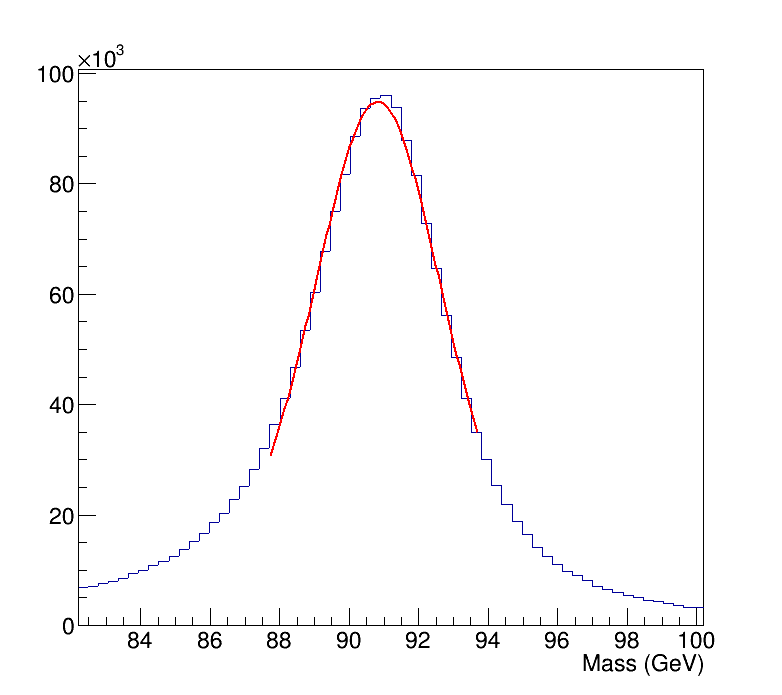
\includegraphics[width=0.55\linewidth]{images/muon_calib/voigt_fit_z_example_w_fit.png}
  \caption[An example fit used for the dimuon mass calibrations.]
   {The dimuon mass distribution is fit around the Z peak for the positively charged muon with $\phi$ between 0 and 0.53.}
  \label{fig:voigt_fit_example}
\end{figure}

As seen in the following sections the Rochester and Kalman filter corrections perform similarly. The search chooses to err on the side of robustness and use the Kalman filter corrections. The Rochester corrections are derived on the Z and should naturally perform a bit better. The Kalman filter corrections are derived on the J/$\Psi$ and Z and are therefore expected to extrapolate to the Higgs peak more reliably. Moreover, the Kalman filter corrections are used in the measurement of $W\rightarrow\mu\nu$, which requires far greater precision on the mass.    

\subsection{Muon Corrections In Data}

The expected behavior of the corrections on the Higgs peak in data is studied by examining the effects on the Z peak in data. Figure \ref{fig:net_data_mu_calib_mean} shows the mean of the fitted Z peak plotted separately vs. $\phi$ for the positively and negatively charged muon for the Rochester, Kalman Filter, and uncorrected Particle Flow measurements. Also shown is the mean plotted  vs. $\eta$ and $p_{t}^\mu$ for the positively and negative charged muon. Finally, the mean is plotted vs. dimuon $p_t$ as well. The corrections should provide consistent measurements of the Z peak in the different $\phi$ and $\eta$ regions of the detector. By aligning the observed mass in $\phi$ and $\eta$, the sets of peaks that make up the inclusive set will align and the net resolution should improve. Note that after corrections, the mean is shifted closer to the theoretical value of 91.2 GeV. Furthermore, the Rochester corrections reduce the variation in phi from 0.1 GeV to 0.0025 GeV, an improvement of 98\%.
\begin{figure}[!h]
  \centering
  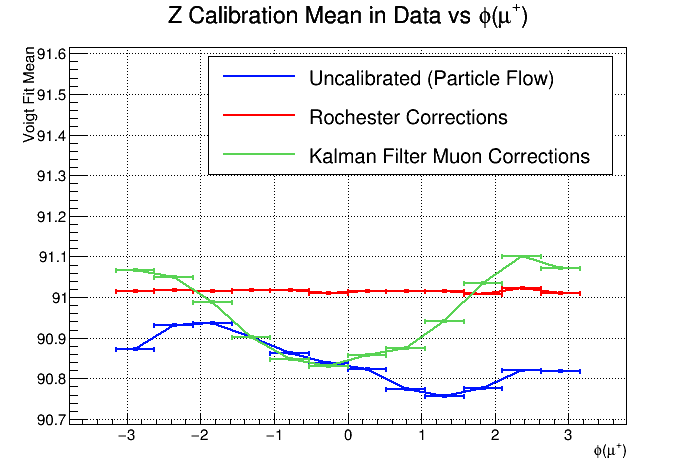
\includegraphics[width=0.32\linewidth]{images/muon_calib/zcal_data_mean_phi_plus.png}
  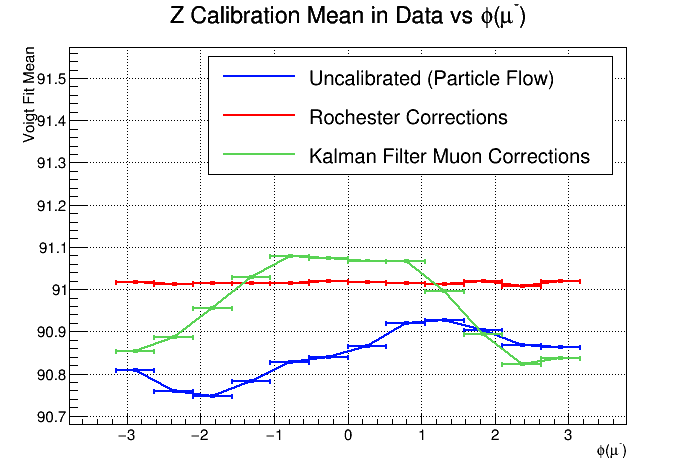
\includegraphics[width=0.32\linewidth]{images/muon_calib/zcal_data_mean_phi_minus.png}
  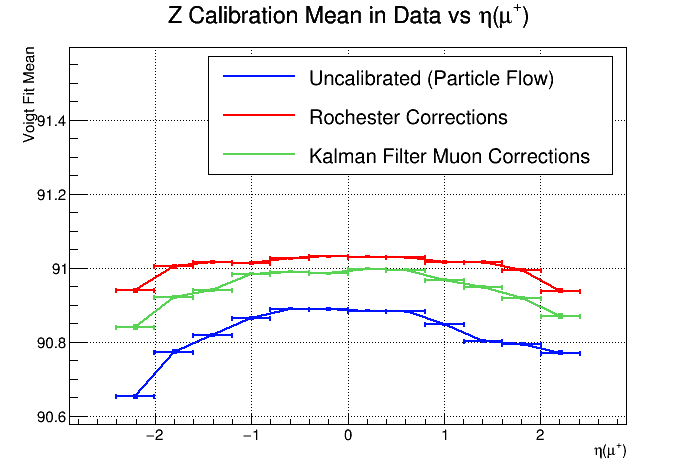
\includegraphics[width=0.32\linewidth]{images/muon_calib/zcal_data_mean_eta_plus.png}
  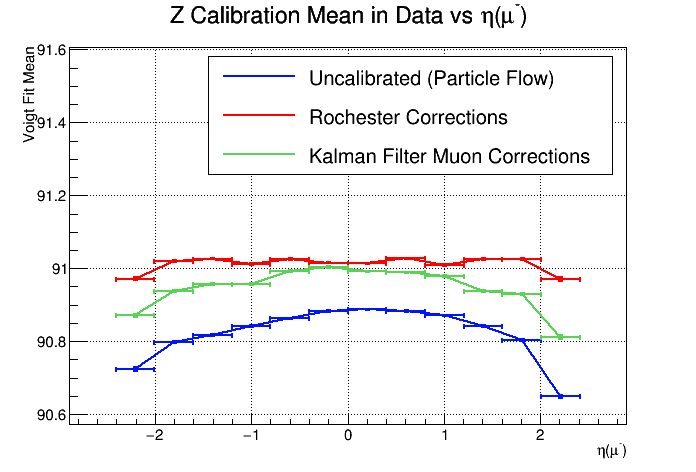
\includegraphics[width=0.32\linewidth]{images/muon_calib/zcal_data_mean_eta_minus.png}
  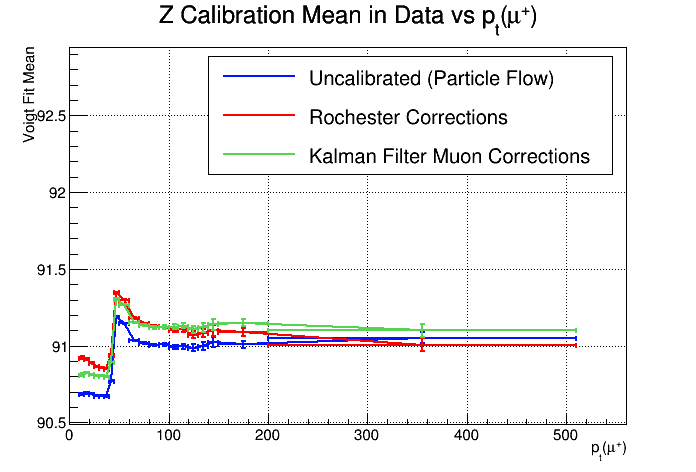
\includegraphics[width=0.32\linewidth]{images/muon_calib/zcal_data_mean_pt_plus.png}
  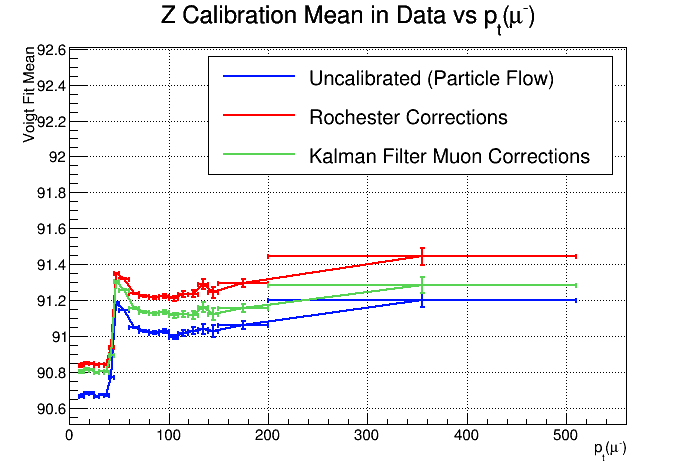
\includegraphics[width=0.32\linewidth]{images/muon_calib/zcal_data_mean_pt_minus.png}
  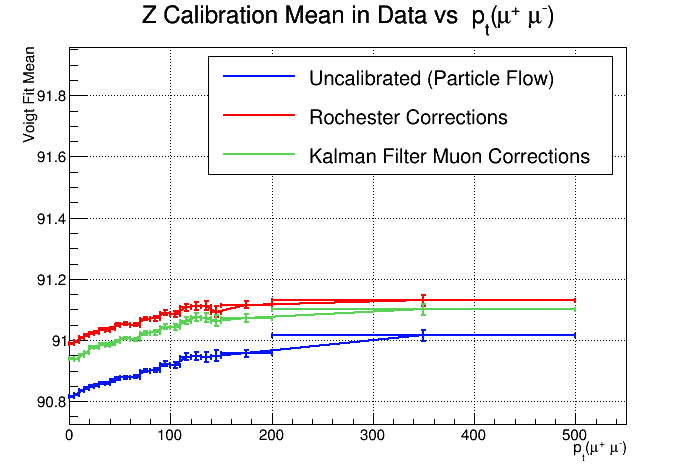
\includegraphics[width=0.32\linewidth]{images/muon_calib/zcal_data_mean_dimu_pt.png}
  \caption[Rochester and Kalman Filter muon corrections on the Z peak mean in data.]
   {The Rochester (Roch) and Kalman Filter (KaMu) muon corrections are applied to data and compared to the uncalibrated Particle Flow (PF) predictions. The fitted mean of the Z peak is plotted  vs. $\phi$, $\eta$, and $p_{t}^\mu$ for the positively and negatively charged muon separately, and for dimuon $p_t$ as well.}
  \label{fig:net_data_mu_calib_mean}
\end{figure}
Figure \ref{fig:net_data_mu_calib_res} shows the Z resolution plotted against the same variables as in Fig.~\ref{fig:net_data_mu_calib_mean}. The Rochester corrections improve the Z resolution by 1.6\%, which translates to about 20 MeV, roughly 4 times the theoretical Higgs width. The Kalman filter corrections improve the resolution in data by 0.076\%, which is about 10 MeV or 2 theoretical Higgs widths.
\begin{figure}[!h]
  \centering
  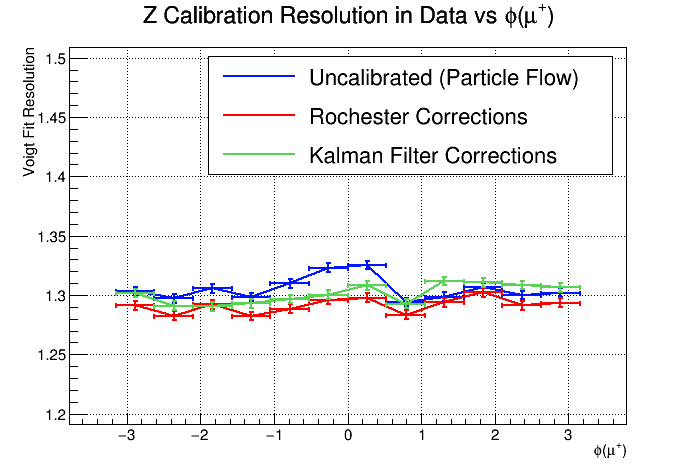
\includegraphics[width=0.32\linewidth]{images/muon_calib/zcal_data_res_phi_plus.png}
  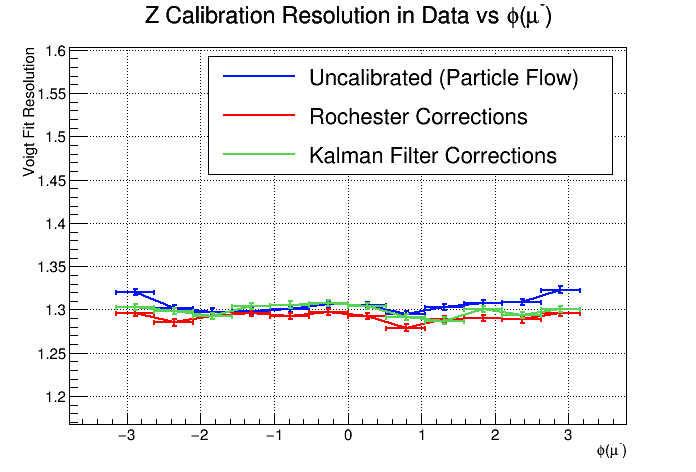
\includegraphics[width=0.32\linewidth]{images/muon_calib/zcal_data_res_phi_minus.png}
  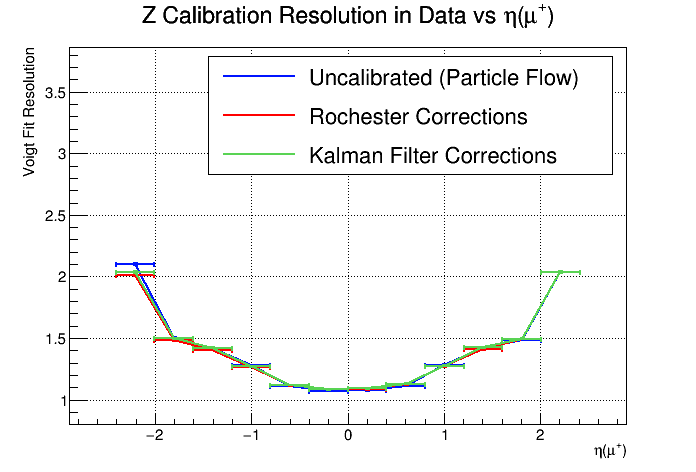
\includegraphics[width=0.32\linewidth]{images/muon_calib/zcal_data_res_eta_plus.png}
  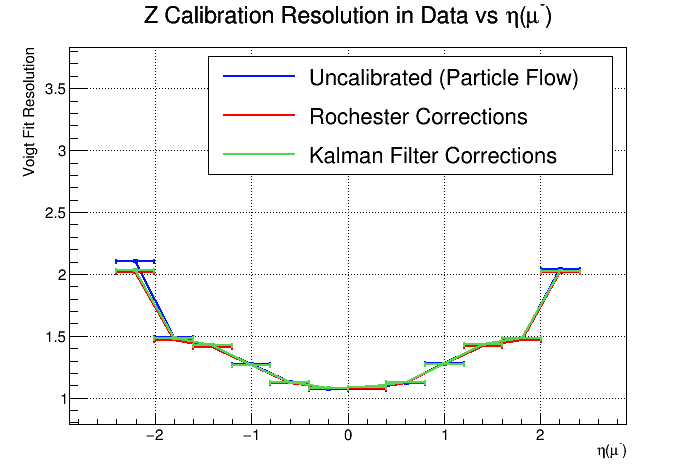
\includegraphics[width=0.32\linewidth]{images/muon_calib/zcal_data_res_eta_minus.png}
  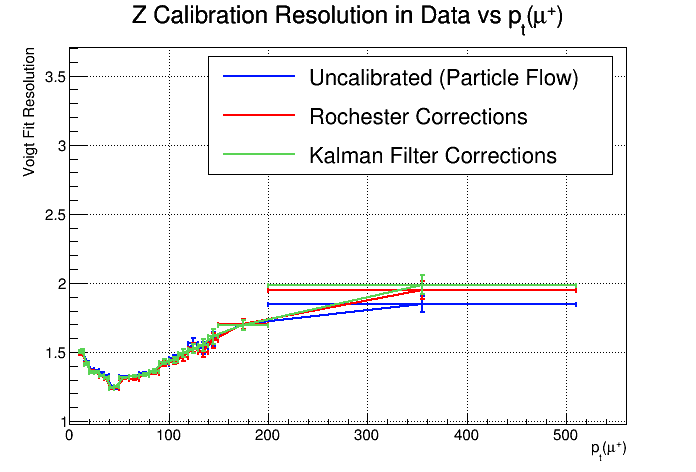
\includegraphics[width=0.32\linewidth]{images/muon_calib/zcal_data_res_pt_plus.png}
  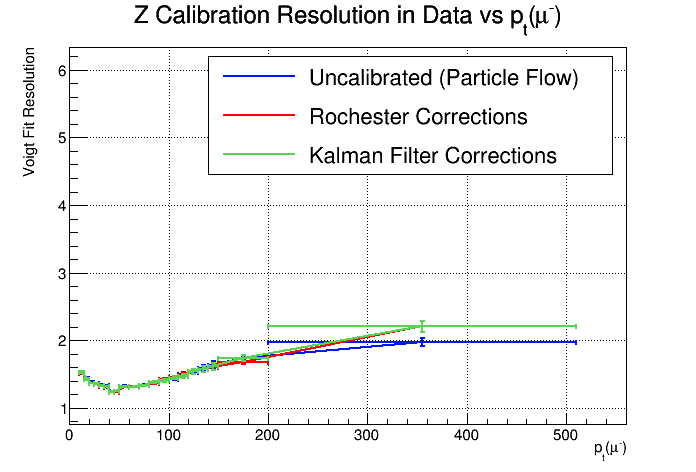
\includegraphics[width=0.32\linewidth]{images/muon_calib/zcal_data_res_pt_minus.png}
  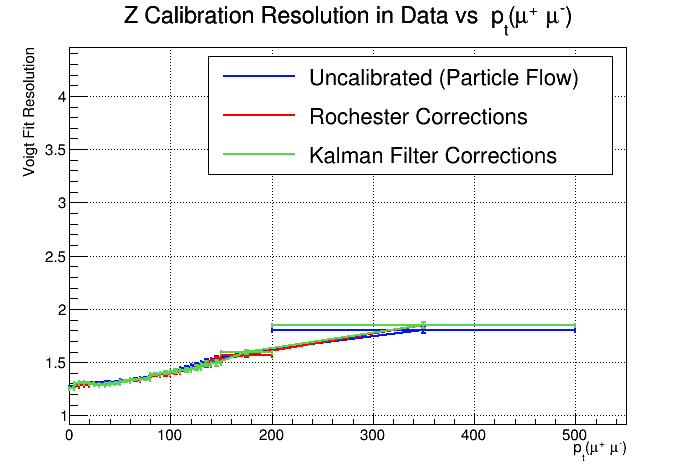
\includegraphics[width=0.32\linewidth]{images/muon_calib/zcal_data_res_dimu_pt.png}
  \caption[Rochester and Kalman filter muon corrections on the Z peak resolution in data.]
   {The Rochester (Roch) and Kalman Filter (KaMu) muon corrections are applied to data and compared to the uncalibrated Particle Flow (PF) measurement. The fitted Z peak resolution is plotted  vs. $\phi$, $\eta$, and $p_t^\mu$ for the positively and negatively charged muon separately, and for the dimuon $p_t$ as well.}
  \label{fig:net_data_mu_calib_res}
\end{figure}

\FloatBarrier
\subsection{Data-MC Agreement In Scale, Resolution}

As aforementioned, the muon corrections should not only improve the resolution of the dimuon mass peaks in data, but align the scale and resolution between data and Monte Carlo as well. With the scale and resolution aligned between MC and data the signal peak (if the hypothesis is true) will appear in data with the width and mass predicted by the MC. When the MC simulates reality accurately, the limits will be set correctly for the different values of the Higgs mass. Figure \ref{fig:data_mc_mean_before} shows the Data/MC agreement on the Z peak mean before any corrections, while Figure \ref{fig:data_mc_roch_mean_after} shows the agreement after Rochester corrections and \ref{fig:data_mc_kamu_mean_after} shows the agreement after the Kalman filter muon corrections. Both the Rochester and Kalman muon corrections successfully align Data/MC in terms of the Z
peak mean.
\begin{figure}[!h]
  \centering
  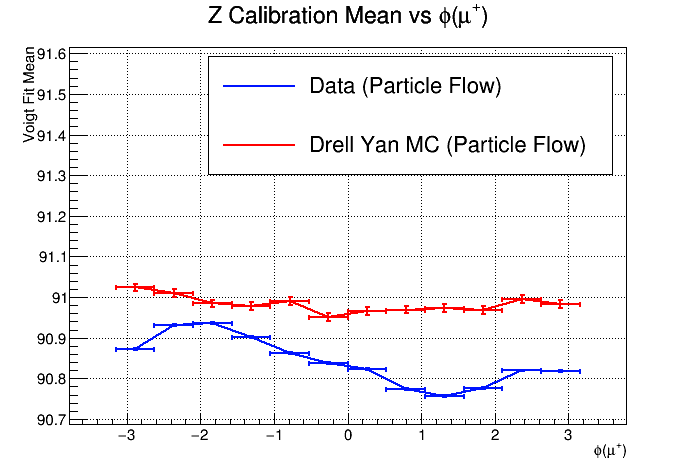
\includegraphics[width=0.32\linewidth]{images/muon_calib/zcal_pf_mc-data_mean_phi_plus.png}
  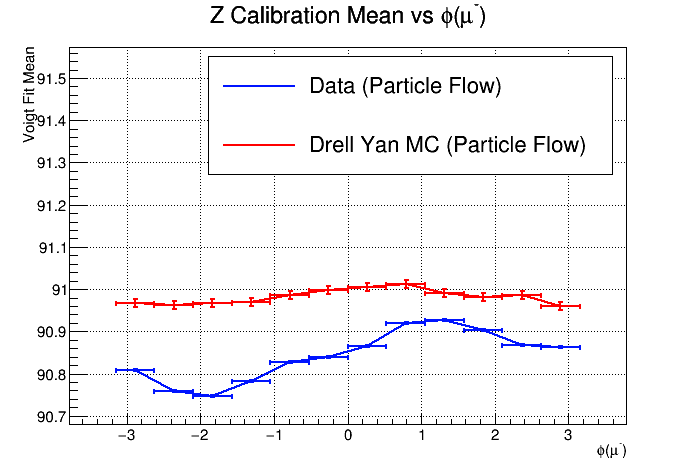
\includegraphics[width=0.32\linewidth]{images/muon_calib/zcal_pf_mc-data_mean_phi_minus.png}
  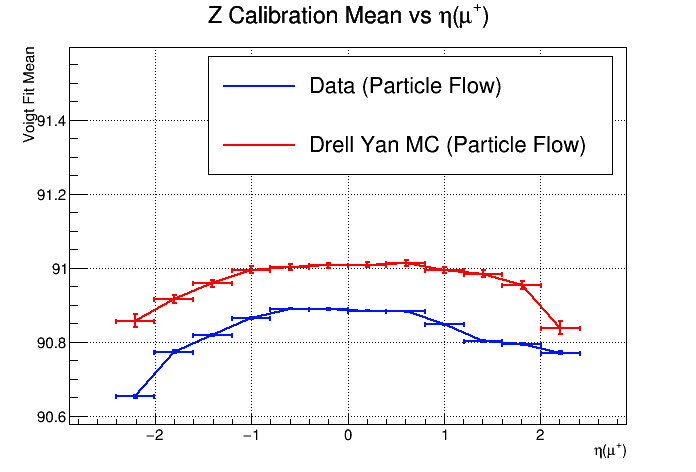
\includegraphics[width=0.32\linewidth]{images/muon_calib/zcal_pf_mc-data_mean_eta_plus.png}
  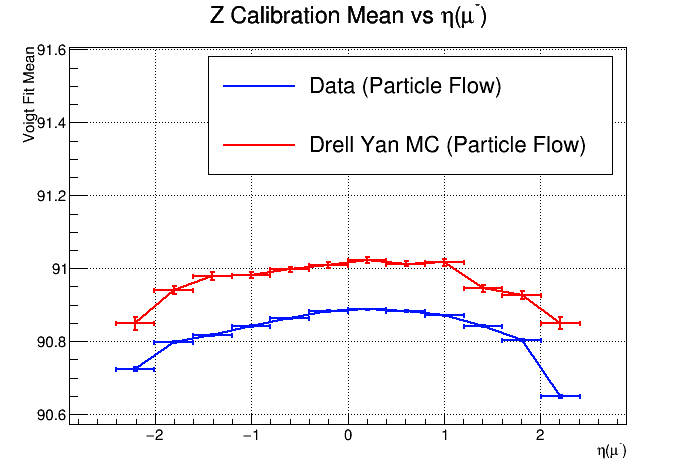
\includegraphics[width=0.32\linewidth]{images/muon_calib/zcal_pf_mc-data_mean_eta_minus.png}
  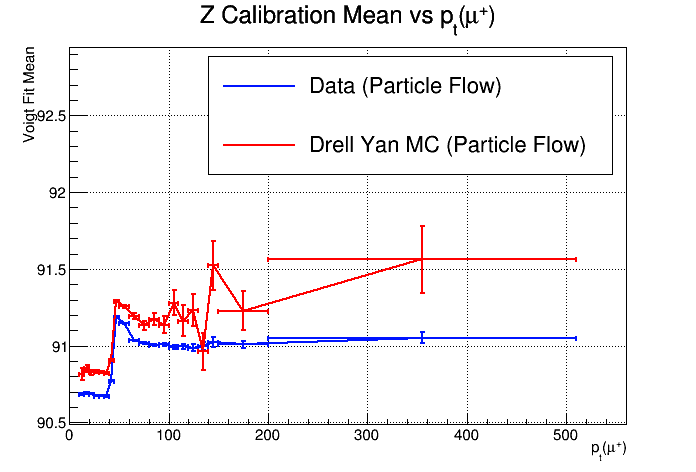
\includegraphics[width=0.32\linewidth]{images/muon_calib/zcal_pf_mc-data_mean_pt_plus.png}
  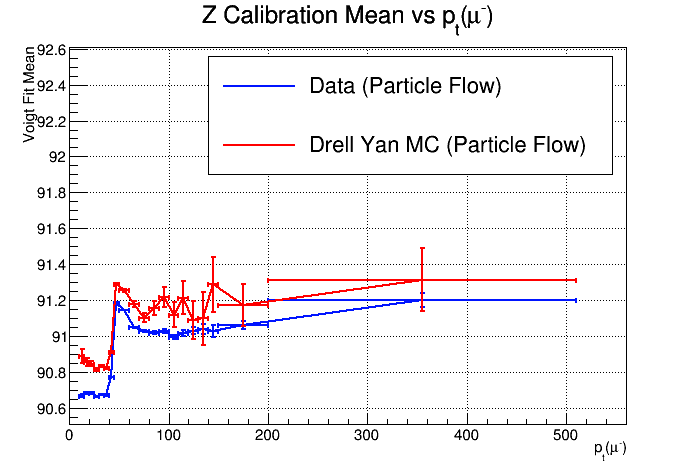
\includegraphics[width=0.32\linewidth]{images/muon_calib/zcal_pf_mc-data_mean_pt_minus.png}
  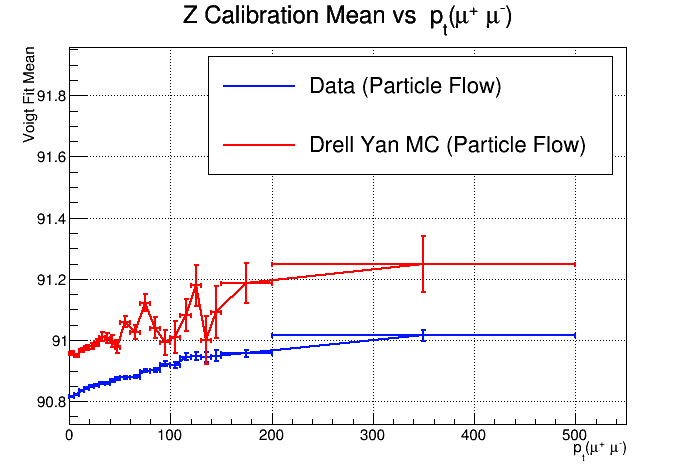
\includegraphics[width=0.32\linewidth]{images/muon_calib/zcal_pf_mc-data_mean_dimu_pt.png}
  \caption[The uncalibrated Z peak mean and its alignment in data and MC.]
   {The fitted mean of the Z peak without any corrections is plotted in data and MC. The mean is plotted vs. $\phi$, $\eta$, and $p_t^\mu$ for the positively and negatively charged muon separately, and for the dimuon $p_t$ as well. Data and MC are not aligned in terms of the Z peak mean before corrections.}
  \label{fig:data_mc_mean_before}
\end{figure}

\begin{figure}[!h]
  \centering
  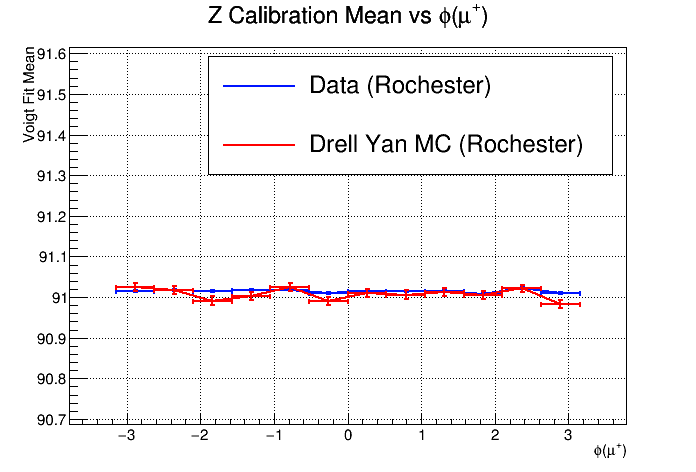
\includegraphics[width=0.32\linewidth]{images/muon_calib/zcal_roch_mc-data_mean_phi_plus.png}
  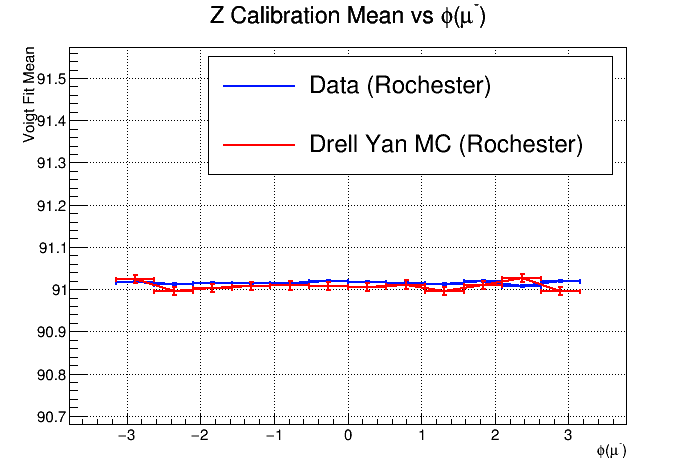
\includegraphics[width=0.32\linewidth]{images/muon_calib/zcal_roch_mc-data_mean_phi_minus.png}
  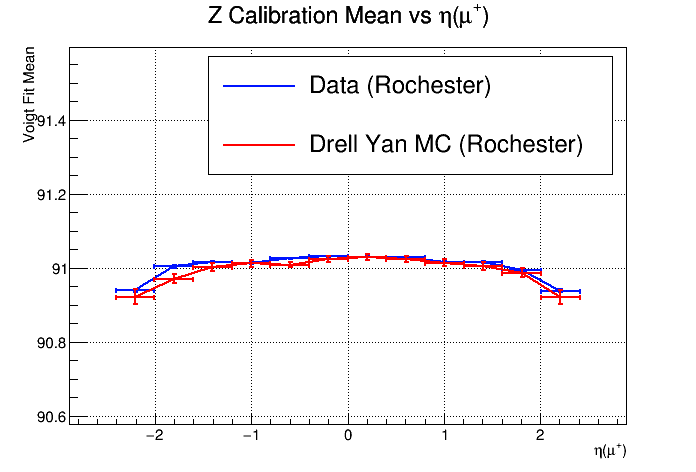
\includegraphics[width=0.32\linewidth]{images/muon_calib/zcal_roch_mc-data_mean_eta_plus.png}
  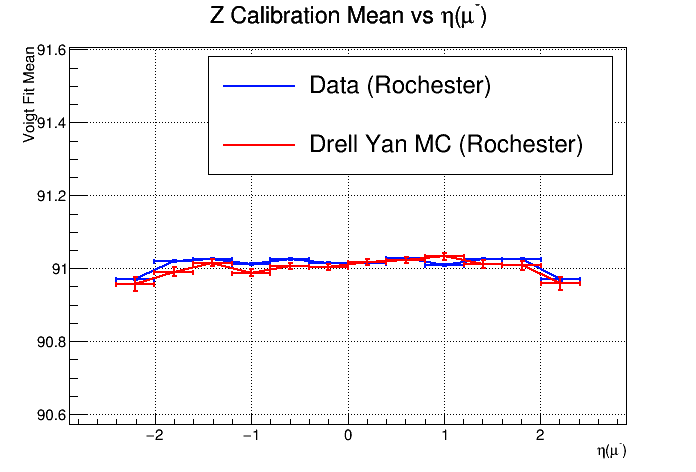
\includegraphics[width=0.32\linewidth]{images/muon_calib/zcal_roch_mc-data_mean_eta_minus.png}
  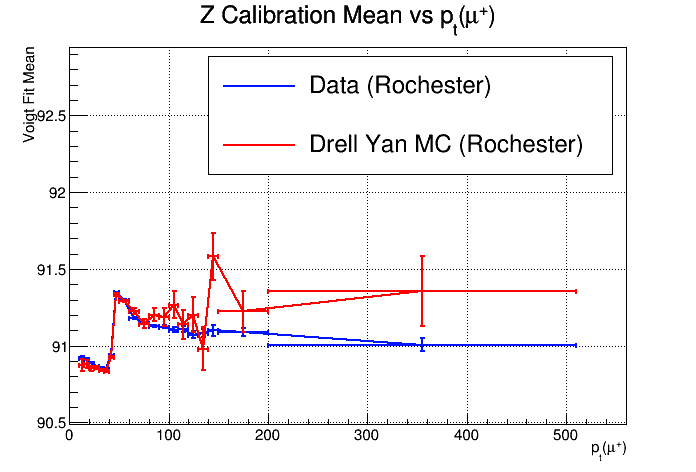
\includegraphics[width=0.32\linewidth]{images/muon_calib/zcal_roch_mc-data_mean_pt_plus.png}
  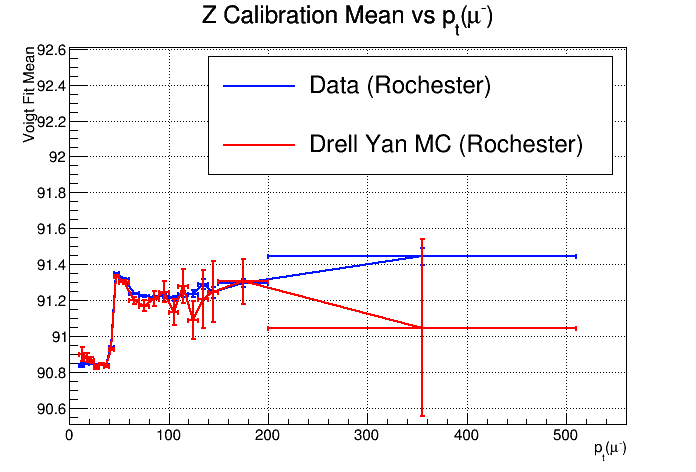
\includegraphics[width=0.32\linewidth]{images/muon_calib/zcal_roch_mc-data_mean_pt_minus.png}
  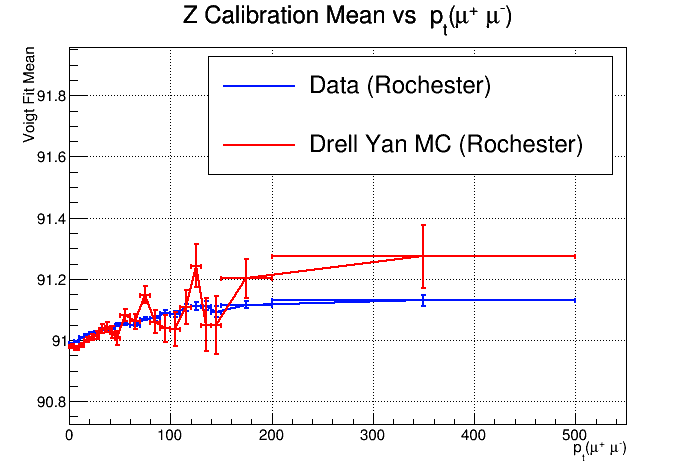
\includegraphics[width=0.32\linewidth]{images/muon_calib/zcal_roch_mc-data_mean_dimu_pt.png}
  \caption[The Z peak mean and its alignment in data and MC after Rochester corrections.]
   {The fitted mean of the Z peak is plotted for the Rochester corrections. The mean is plotted in data and MC vs. $\phi$, $\eta$, and $p_t^\mu$ for the positively and negatively charged muon separately, and for the dimuon $p_t$ as well. Data and MC align very well in terms of the Z peak mean after applying the Rochester muon corrections.}
  \label{fig:data_mc_roch_mean_after}
\end{figure}

\begin{figure}[!h]
  \centering
  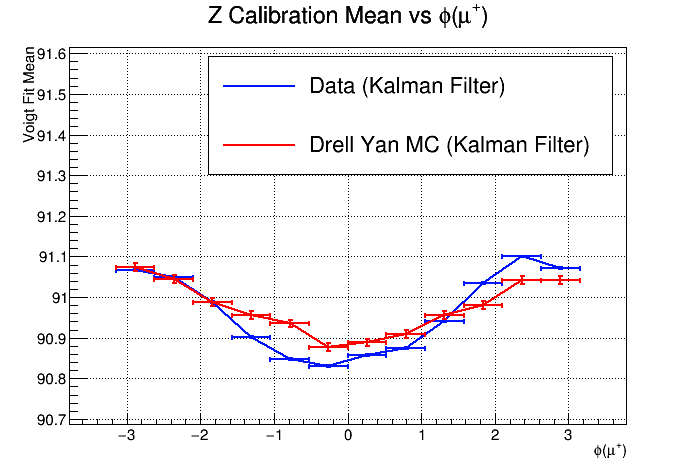
\includegraphics[width=0.32\linewidth]{images/muon_calib/zcal_kamu_mc-data_mean_phi_plus.png}
  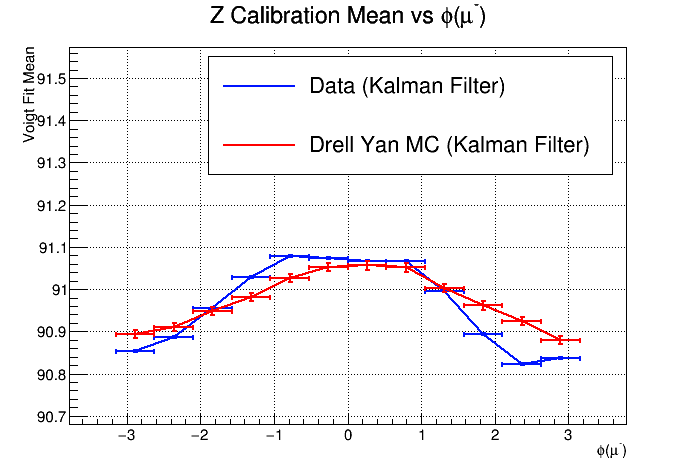
\includegraphics[width=0.32\linewidth]{images/muon_calib/zcal_kamu_mc-data_mean_phi_minus.png}
  \includegraphics[width=0.32\linewidth]{images/muon_calib/zcal_kamu_mc-data_mean_eta_plus.png}
  \includegraphics[width=0.32\linewidth]{images/muon_calib/zcal_kamu_mc-data_mean_eta_minus.png}
  \includegraphics[width=0.32\linewidth]{images/muon_calib/zcal_kamu_mc-data_mean_pt_plus.png}
  \includegraphics[width=0.32\linewidth]{images/muon_calib/zcal_kamu_mc-data_mean_pt_minus.png}
  \includegraphics[width=0.32\linewidth]{images/muon_calib/zcal_kamu_mc-data_mean_dimu_pt.png}
  \caption[The Z peak mean and its alignment in data and MC after Kalman Filter corrections.]
   {The fitted mean of the Z peak is plotted for the Kalman Filter corrections. The mean is plotted in data and MC vs. $\phi$, $\eta$, and $p_t^\mu$ for the positively and negatively charged muon separately, and for the dimuon $p_t$ as well. Data and MC align very well in terms of the Z peak mean after applying the Kalman filter muon corrections.}
  \label{fig:data_mc_kamu_mean_after}
\end{figure}
Both corrections also succeed in aligning the Z peak resolution. The mismatch before corrections is seen in Figure \ref{fig:data_mc_res_before} and the agreement after corrections is seen in Figure \ref{fig:data_mc_roch_res_after} and Figure \ref{fig:data_mc_kamu_res_after}.
\begin{figure}[!h]
  \centering
  \includegraphics[width=0.32\linewidth]{images/muon_calib/zcal_pf_mc-data_res_phi_plus.png}
  \includegraphics[width=0.32\linewidth]{images/muon_calib/zcal_pf_mc-data_res_phi_minus.png}
  \includegraphics[width=0.32\linewidth]{images/muon_calib/zcal_pf_mc-data_res_eta_plus.png}
  \includegraphics[width=0.32\linewidth]{images/muon_calib/zcal_pf_mc-data_res_eta_minus.png}
  \includegraphics[width=0.32\linewidth]{images/muon_calib/zcal_pf_mc-data_res_pt_plus.png}
  \includegraphics[width=0.32\linewidth]{images/muon_calib/zcal_pf_mc-data_res_pt_minus.png}
  \includegraphics[width=0.32\linewidth]{images/muon_calib/zcal_pf_mc-data_res_dimu_pt.png}
  \caption[The uncalibrated Z peak resolution in data and MC.]
   {The fitted resolution of the Z peak without corrections is plotted. The resolution is plotted in data and MC vs. $\phi$, $\eta$, and $p_t^\mu$ for the positively and negatively charged muon separately, and for the dimuon $p_t$ as well. Data and MC do not show similar resolutions for the Z peak before corrections.}
  \label{fig:data_mc_res_before}
\end{figure}
\begin{figure}[!h]
  \centering
  \includegraphics[width=0.32\linewidth]{images/muon_calib/zcal_roch_mc-data_res_phi_plus.png}
  \includegraphics[width=0.32\linewidth]{images/muon_calib/zcal_roch_mc-data_res_phi_minus.png}
  \includegraphics[width=0.32\linewidth]{images/muon_calib/zcal_roch_mc-data_res_eta_plus.png}
  \includegraphics[width=0.32\linewidth]{images/muon_calib/zcal_roch_mc-data_res_eta_minus.png}
  \includegraphics[width=0.32\linewidth]{images/muon_calib/zcal_roch_mc-data_res_pt_plus.png}
  \includegraphics[width=0.32\linewidth]{images/muon_calib/zcal_roch_mc-data_res_pt_minus.png}
  \includegraphics[width=0.32\linewidth]{images/muon_calib/zcal_roch_mc-data_res_dimu_pt.png}
  \caption[The Z peak resolution's alignment in data and MC after Rochester corrections.]
   {The fitted resolution of the Z peak is plotted for the Rochester corrections. The resolution is plotted in data and MC vs. $\phi$, $\eta$, and $p_t^\mu$ for the positively and negatively charged muon separately, and for the dimuon $p_t$ as well. After Rochester corrections, data and MC have similar resolutions for the Z peak.}
  \label{fig:data_mc_roch_res_after}
\end{figure}
\begin{figure}[!h]
  \centering
  \includegraphics[width=0.32\linewidth]{images/muon_calib/zcal_kamu_mc-data_res_phi_plus.png}
  \includegraphics[width=0.32\linewidth]{images/muon_calib/zcal_kamu_mc-data_res_phi_minus.png}
  \includegraphics[width=0.32\linewidth]{images/muon_calib/zcal_kamu_mc-data_res_eta_plus.png}
  \includegraphics[width=0.32\linewidth]{images/muon_calib/zcal_kamu_mc-data_res_eta_minus.png}
  \includegraphics[width=0.32\linewidth]{images/muon_calib/zcal_kamu_mc-data_res_pt_plus.png}
  \includegraphics[width=0.32\linewidth]{images/muon_calib/zcal_kamu_mc-data_res_pt_minus.png}
  \includegraphics[width=0.32\linewidth]{images/muon_calib/zcal_kamu_mc-data_res_dimu_pt.png}
  \caption[The Z peak resolution's alignment in data and MC after Kalman Filter corrections.]
   {The fitted resolution of the Z peak is plotted for the Rochester corrections. The resolution is plotted in data and MC vs. $\phi$, $\eta$, and $p_t^\mu$ for the positively and negatively charged muon separately, and for the dimuon $p_t$ as well. After Kalman filter muon corrections, data and MC have similar resolutions for the Z peak.}
  \label{fig:data_mc_kamu_res_after}
\end{figure}

\FloatBarrier
\subsection{Derivation Of Systematic Uncertainties}

Uncertainties are provided both for Kalman fiter muon corrections and Rochester corrections.
For the Kalman filter corrections, uncertainties include the non-closure on data. Histograms of the Kalman filter's most probable true mass value for the signal MC events are shown in Figure \ref{fig:shifts_scale} for the least sensitive and most sensitive categories. No particular structure is observed as a function of category or production process. A conservative number of $0.05\%$ is used for the scale uncertainty. Resolution corrections derived with the Kalman filter corrections have an uncertainty of $10\%$.
\begin{figure}[!h]
    \centering
    \includegraphics[width=0.49\textwidth]{images/muon_calib/syst_GluGlu_cat0.png}
    \includegraphics[width=0.49\textwidth]{images/muon_calib/syst_GluGlu_cat12.png}
    \caption[Kalman filter statistical uncertainty on the dimuon mass.]
    {The Kalman filter's most probable true mass values are plotted for the signal MC. The least sensitive category is shown on the left and the most sensitive category is shown on the right.}
    \label{fig:shifts_scale} T
\end{figure}
%%%%%%%%%%%%%%%%%%%%%%%%%%%%%%%%%%%%%%%%%%%%%%%%%%%%%%%
\section{Event Selection, Object Reconstruction, And Further Corrections}

The Particle Flow (PF) algorithm reconstructs the detector level measurements at CMS into higher level objects like electrons, muons, photons, and jets. The $H\rightarrow\mu^+\mu^-$ search uses the PF muons, jets, and missing transverse energy (MET) with four vector information like E, $p_t$, $\eta$, and $\phi$ to perform the analysis. Certain selections are made to reduce the size of the data while keeping the signal events. In addition, the $\eta$ coverage of the subdetectors limits the available data for different objects. The analysis follows the Physics Object Group (POG) recommendations for 2016. 

\subsection{Muons}
The PF algorithm forms muon objects by matching hits in the silicon tracker with hits in the muon chambers. Because the muon chambers end at $|\eta|=2.4$, the analysis is limited to muons with $|\eta| \leq 2.4$. Moreover, the $H\rightarrow\mu^+\mu^-$ signal is expected to occur around 125 GeV, which on average has 62 GeV muons. As such, the analysis requires muons with $p_t \geq 20$ GeV. Some muons originate from hadronic decays, surrounded by activity, while the signal produces isolated muons directly from the Higgs decay. To eliminate the hadronic muon background, only energetically isolated muons are considered. The isolation is determined by considering the energetic activity in a cone $\Delta R\equiv\sqrt{\Delta\eta^{2}+\Delta\phi^{2}}<0.4$ relative to the muon's $p_T$,
\begin{equation}
I_{rel}^{PF}=(p_{T}^{ch}+\max(0,E_{T}^{\gamma}+E_{T}^{nh}-0.5*p_{T}^{chPU}))/p_{T}^{\mu}.
\end{equation}
The term $p_{T}^{ch}$ is the sum of the charged hadron $p_T$ excluding hadrons from pile-up vertices,
$E_{T}^{\gamma}$ is the sum of the photon $E_t$, and $E_{T}^{nh}$ is the sum of the neutral hadron transverse
energy. The $0.5p_{T}^{chPU}$ term estimates the energy contribution from neutral pile-up as half the $p_t$ of the charged pile-up.
Muons with $I_{rel}^{PF} < 0.25$ in the cone are kept. In order to remove cosmic ray muons, muons from mid-flight decays, hadronic punch through, and muons with a poor $p_t$ assignment, only muons that pass the Medium ID are considered. 

\subsection{Jets And MET}
Jets are used to distinguish the VBF channel from the overwhelming Drell-Yan background. To avoid fake jets from hot calorimeter cells and readout effects, the jets must pass the Loose ID requirements. Moreover, to distinguish hard scattering jets from pile-up, the jets must also pass the Loose Pile-Up ID. Forward jets are especially indicative of VBF events, and the forward hadronic calorimeter goes all the way up to $|\eta| = 4.7$, so all jets with $|\eta| \leq 4.7$ are considered. High $p_t$ jets are better measured and better distinguish VBF from Drell-Yan, so in order to keep these jets without being inundated, jets must have a $p_T \geq 30$ GeV. Some objects PF declares to be jets may actually be muons, so any jet within a $\Delta R = 0.4$ a muon is not considered. All of the jets used in the analysis are anti-k$_t$ PF jets with a distance parameter of 0.4. 

Jets tagged as bottom quarks are used to reduce $t\bar{t}$ background. To this end, the analysis uses the centrally provided combined secondary vertex b-tagging algorithm (CSVv2) to identify likely b-jets. The CSVv2 medium working point is used, providing a 60\% efficiency (true-positive) for b-jets, and a misidentification (false-positive) rate of about 1\% for u, d, s, and gluon jets. The silicon tracker is needed to identify the secondary vertices corresponding to b-jets, and this subdetector ends at $|\eta|=2.4$. Therefore the b-tagging algorithm is only applied to jets with $|\eta| \leq 2.4$.

The $H\rightarrow\mu^+\mu^-$ search also uses the MET to reduce the $t\bar{t}$ background. By conservation of momentum, the $\vec{p}_t$ for all of the particles in an event should add up to zero. A non-zero $\vec{p}_t$ indicates that detector missed the $p_t$ from some undetected neutral particles. The $|\vec{p}_t|$ associated with the "invisible" particles like neutrinos is called the MET\footnote{MET usually corresponds to neutrinos which have a tiny mass and a $p_t$ basically equal to the $E_t$.}

\subsection{Pile-up Reweighting}
Pile-up (PU) refers to particles emerging from collision vertices other than the vertex of interest. With high pile-up there are many more hits in the detector and the chance to misassign different quantities increases. As a consequence, discrepancies in the PU distributions between data and MC propagate to create discrepancies in the variables used in the analysis. To correct the PU and the concomitant effects, the MC is reweighted to match the data in the PU spectrum. 
\subsection{Muon Efficiency Scale Factors}
In data, only a certain percentage of events that should pass the muon trigger, isolation, and ID requirements actually succeed. This probability is called the efficiency, and labelled $\varepsilon$. To correct the efficiency in the MC samples, scale factors (SFs) are applied to the MC events by $p_t$ and $\eta$ to scale the efficiency to the efficiency observed in data.  

When there are multiple muons in an event, only one has to pass the trigger criteria, and the probability that at least one passes is given by $\varepsilon_\textup{trg}=1 - \prod_{i=1}^{N}{{(1-\varepsilon_{\mu}}_{i})}$, where N is the total number of trigger matched muons with $p_t \geq 26$ GeV. The trigger SF is then,  
\begin{equation}
    \label{eqn:sf_trg}
    \textup{SF}_\textup{trg} = \frac{\varepsilon_\textup{trg}^\textup{data}}{\varepsilon_\textup{trg}^\textup{MC}}.
\end{equation}
On the other hand, every muon in the event must pass the isolation and ID requirements. These efficiencies are given by $\varepsilon_\textup{id/iso} = \prod_{i=1}^{N} \varepsilon_{\mu,i}$, where N is the number of muons, and the SFs are,
\begin{equation}
    \label{eqn:sf_id_iso}
    \textup{SF}_\textup{id/iso} = \frac{\varepsilon_\textup{id/iso}^\textup{data}}{\varepsilon_\textup{id/iso}^\textup{MC}}.
\end{equation}
The efficiencies in data are different for data taking runs B through F compared to G and H, so the final scale factors are given by the weighted average,
\begin{align}
    w_\textup{BF} &= \frac{\mathcal{L}_\textup{BF}}{\mathcal{L}_\textup{tot}} \\
    w_\textup{GH} &= \frac{\mathcal{L}_\textup{GH}}{\mathcal{L}_\textup{tot}} \\
    \label{eqn:sf}
    \textup{SF} &= w_\textup{BF} \cdot \left( \textup{SF}_\textup{trg}^\textup{BF} \textup{SF}_\textup{id}^\textup{BF} \textup{SF}_\textup{iso}^\textup{BF}\right) 
    + w_\textup{GH}\cdot \left( \textup{SF}_\textup{trg}^\textup{GH} \textup{SF}_\textup{id}^\textup{GH} \textup{SF}_\textup{iso}^\textup{GH}\right).
\end{align}
The scale factors are centrally provided by the Muon POG, and the weights are determined by the integrated luminosity.
\subsection{Jet, MET, And B-tagging Corrections}
Centrally provided corrections from the JetMET POG correct the jet energy to remove residual pile-up contributions, to reinstate known energy loss from reconstruction effects, and to align data and MC. The corrections are propagated to the Missing Transverse Energy (MET). While the MET is often physical, large values may arise due to reconstruction issues like cosmic ray muons, noise, or beam-halo particles. To remove these contributions to the reported MET value, the POG recommended MET filters are applied. 

The JetMET POG also provides MC scale factors accounting for data/MC discrepancies in b-tagging efficiency and misidentification. A single SF for each MC event accounts for all of the jets in the event and their flavors (u,d,s,c,g) using the underlying MC truth information. 

\subsection{Event Selection}

In order to consider a proton-proton event in the analysis, the event must have two oppositely charged muons from the primary vertex, with one muon matching either the HLT-IsoMu-24 or the HLT-IsoTkMu-24 trigger. The trigger matched muon must have a $p_T > 26$ GeV. The triggers chosen are the lowest $p_T$, unprescaled triggers available for the entire data taking period. In addition, the event must have a least one valid Primary Vertex (PV). The PV for the event is the one with the largest scalar sum of the $p^2_t$ and at least four associated tracks.  

\chapter{OPTIMIZING THE SENSITIVITY OF THE $H\rightarrow\mu^+\mu^-$ SEARCH} \label{optimize}

This chapter covers the work to optimize the sensitivity of the analysis. The work on the Level-1 Muon Trigger is covered first, and the classification and categorization of events is covered after. The work on the trigger improves the sensitivity by increasing the amount of data available to the $H\rightarrow\mu^+\mu^-$ search, and the classification and categorization of events groups the events to maximize the chance of discovery.  

\section{Improving The Level-1 Muon Trigger}

Saving as much relevant data as possible is important as the chance of discovery improves with a larger dataset. With this in mind, improvements are made to the L1 Muon Trigger to improve its capability to save events with high momentum muons and discard events without them. Towards this end, Boosted Decision Trees (BDTs) are trained to distinguish high momentum muons from low momentum muons. The BDTs are loaded onto Field Programmable Gate Arrays (FPGAs) in the L1 Muon Trigger and run online. The improvements increase the amount of data with high momentum muons available for the $H\rightarrow \mu^+\mu^-$ search. 

The LHC collides bunches of protons every 25 ns at a center of mass energy of 13 TeV. The CMS experiment detects the resulting particles and measures their kinematics using a variety of subdetectors working in concert. With 40 million proton bunch crossings per second amounting to roughly 40 TB of data each second, saving the information from every event is not feasible. As such, the CMS trigger system chooses the interesting events to save to disk, operating in two stages \cite{Khachatryan:2016bia}. The Level-1 (L1) trigger runs in hardware online reducing the throughput of data from 40 MHz to 100 KHz. From there, the High Level Trigger (HLT) operates in software online reducing the rate from 100 KHz to 1 KHz. In the end, about 1 GB/s is saved to disk.

With 40 MHz of input, the L1 Trigger has only 4 $\mu$s to decide whether to keep the information for an event. The Endcap Muon Track Finder (EMTF) -- part of the L1 Trigger dedicated to muons -- has only about 500 ns to determine the location, tracks, and momentum of the muons passing through the Cathode Strip Chambers (CSC) and Resistive Plate Chambers (RPC) in the endcaps of CMS \cite{Tapper:1556311}. High momentum muons are an important object for many physics analyses at CMS and the most important object for $H\rightarrow\mu^+\mu^-$. As such, an accurate momentum assignment distinguishing low momentum muons (background) from high momentum muons (signal) is key to the L1 Trigger. In order to meet the timing requirements, the EMTF's logic is implemented in Field Programmable Gate Arrays (FPGAs), a type of reprogrammable hardware that allows vast parallelization and speeds much greater than even the best CPUs.

To improve the transverse momentum ($p_t$) assignment for muons in the endcaps at Level-1, the EMTF team trained Boosted Decision Trees (BDTs) offline using TMVA \cite{Hocker:2007ht}, and stored the prediction scheme into a 1.2 GB Look-Up Table (LUT). The FPGAs then use the LUT online to assign the $p_t$ in a single operation. Using the LUT to turn the BDT $p_t$ assignment into a simple look-up enables the EMTF to utilize the power of a robust machine learning algorithm for its momentum predictions while still operating at the required time scale. Putting a parallelized version of the BDTs directly into the FPGAs, while hypothetically possible, would require more than the available number of logic gates. Such an implementation would still be slower than the LUT method, and changing the $p_t$ assignment would require reprogramming the FPGA logic each time. The LUT method provides a simple way to run any machine learning evaluation at high speed by turning the evaluation into a single operation.

\subsection{Metrics Of Success}

Two metrics are used to measure the success of the EMTF: the rate and the efficiency. The rate at X GeV is defined as the number of muons with a predicted $p_t$ greater than X GeV. In other words, the rate consists of both true and false positives above the $p_t$ threshold. The efficiency at X GeV is defined as the number of muons with both predicted $p_t$ and true $p_t$ greater than X GeV divided by the number of muons with true $p_t$ above X GeV. Put another way, the efficiency measures the percentage of muons with true $p_t$ above X GeV correctly predicted above X GeV. A good trigger will minimize the data saved without losing the interesting high $p_t$ events where unexplored physics lies, i.e. it will minimize rate while maximizing the efficiency.

\subsection{The EMTF Regression Project}

A muon traveling through the endcap detectors has a chance to leave hits in four sequential stations labeled 1, 2, 3, and 4. The specific combination of hits like 1,3,4 is called the mode. Each station records the $\phi$ and $\theta$ location of a hit, among other information. The CSCs have better spatial resolution, so the $\phi$ and $\theta$ information is taken from the CSCs by default, but the RPC measurements for the station are used if the CSCs missed the hit in the same station. The charged muons travel through a magnetic field following curved paths due to the Lorentz force. The force causes the high $p_t$ muons in a magnetic field to bend less and the low $p_t$ muons to bend more. The difference in $\phi$ and $\theta$ between stations i and j, $\Delta\phi_{ij}$ and $\Delta\theta_{ij}$, quantify the curvature of the track. With most of the curvature accounted for by the $\Delta\phi$ variables, the $\Delta\phi$s provide the majority of the $p_t$ discrimination.

A major difficulty in minimizing the rate is the steeply falling $p_t$ distribution. A typical interesting event has $p_t$ greater than 25 GeV, and there are about one thousand 5 GeV muons for every 25 GeV muon. With so many more low $p_t$ events, predicting the low momentum muons poorly will drastically increase the rate. Moreover, in addition to the large number of low $p_t$ muons, there are other noteable difficulties: the muons travel through a non-uniform magnetic field, some scatter between detector stations, and those with high $p_t$ often shower charged particles upon interacting with the detector material. Moreover, low $p_t$ muons may spiral completely before getting to the next station. The scattering, showering, and spiraling add noise to the underlying true behavior, while the number of low $p_t$ muons requires that the regression focus on the low momentum regime to prevent an explosion in the rate.

In order to assign $p_t$ in a robust way and deal with the aforementioned difficulties, a BDT is trained for each possible mode using the discretized values for the features of Table \ref{tab:bits}. The loss function and weights are chosen to focus on the low $p_t$ events and minimize the rate while maintaining acceptable efficiency. Features are chosen for each mode to give the BDT the information needed to predict the $p_t$ while dealing with the non-uniform magnetic field and the problematic scattering and showering effects.

The $\Delta\phi$ variables available for each mode are used as features to determine the curvature and get most of the $p_t$ discrimination. However, the power of these variables depends largely on the track position in $\theta$. The magnetic field varies as a function of $\theta$ affecting the magnitude of the curvature for a given $p_t$, thus correlating $\Delta\phi$, $p_t$, and $\theta$. The link between these three makes $\theta$ the next most important training feature.

Variables modeling the mean and RMS of the available $\Delta\phi$s for the mode are also used as features in order to identify scattering and showering effects. If a muon were to scatter or shower between stations the recorded hit in a station may not be the true hit of the muon. Any $\Delta\phi$ involving this station will be an outlier. To determine the severity of the deviation and the likelihood of scattering/showering, the idea is to identify the outlier station and to compare the mean and RMS $\Delta\phi$ with and without the outlier station. The greater the difference the greater the severity. The nominal mean and RMS $\Delta\phi$ features are calculated using all available $\Delta\phi$s for the mode. The exclusive mean and RMS are calculated using all available $\Delta\phi_{ij}$ for the mode with i or j $\neq$ $S_{out}$, where $S_{out}$ is the outlier station. $S_{out}$ is the excluded station such that leaving it out of the sum minimizes the mean and RMS. The outlier station, $S_{out}$, is also used as a feature. Including the nominal mean and RMS of $\Delta\phi$, the exclusive RMS and mean of $\Delta\phi$, and $S_{out}$ as features helps the BDT differentiate scattering, showering, and normal events.

The features described above are the most important features, but not the whole collection. The front-rear (FR) bit designates whether the muon hit a front or rear CSC chamber in the station, and it is also included. The $\Delta\theta$s provide additional curvature information, and these are included as well. The $B$ feature for each station is included as well, and it flags whether the $\phi$, $\theta$ information for the station came from the CSCs or the RPCs. If there are bits available for the $B_i$ feature it also includes information about the single station $\Delta\phi$ bend angle within a CSC chamber. Lastly, the $+/-$ feature stores the signs of the later $\Delta\phi$s relative to the first $\Delta\phi_{ij}$ for the mode.

\subsection{Putting The BDTs Into A Look-up Table}

After training BDTs for each mode, the mode and the fundamental features from which the others can be derived are discretized and fit into a 30 bit word. The discretization scheme is different for each mode, detailed in Table \ref{tab:bits}. With the feature space compressed into 30 bits, there are $2^{30}$ possibilities that need to be assigned a $p_t$. A LUT is created by looping over all $2^{30}$ possible bit words, decoding each word into the fundamental features, deriving the secondary features, and sending the values to the BDT to assign the $p_t$ prediction. Using 9 bits for the $p_t$, this amounts to a 1.2 GB LUT where each bit word value is an address and the $p_t$ is the value in memory. Discretizing the feature space and creating a LUT turns the $p_t$ assignment into a single operation. The LUT is then used by the FPGA logic online to assign $p_t$ to muon tracks in the EMTF. The LUT method is a simple way to run any machine learning method quickly, but compressing the features into 30 or so bits may not always be feasible for the application.

\begin{table}[htb]
   \caption{The feature discretization scheme for each mode.}
   \label{tab:bits}
   \textbf{Four Station Modes}
\\[\baselineskip]
   \begin{tabular}{ l  l  l  l  l  l  l  l  l  l  l  l  l  l}
   \hline
   Mode & Feature & $\Delta\phi_{12}$ & $\Delta\phi_{23}$ & $\Delta\phi_{34}$ & +/- & $\Delta\theta_{14}$
                                              & $B_1$ & $B_2$ & $B_3$ & $B_4$ & $FR_1$ & $\theta$ & Mode \\ \cline{2-14}
   1-2-3-4 & Bits & 7 & 5 & 4 & 2 & 2 & 2 & 1 & 1 & 1 & 1 & 3 & 1 \\ 
   \hline
   \end{tabular}
\\[\baselineskip]
   \textbf{Three Station Modes}
%   \\ \\
\\[\baselineskip]
   \begin{tabular}{ l  l  l  l  l  l  l  l  l  l  l  l  l}
   \hline
   Mode & Feature & $\Delta\phi_{12}$ & $\Delta\phi_{23}$ & +/- & $\Delta\theta_{13}$
                                            & $B_1$ & $B_2$ & $B_3$ & $FR_1$ & $FR_2$ & $\theta$ & Mode \\ \cline{2-13}
   1-2-3 & Bits & 7 & 5 & 1 & 3 & 2 & 1 & 1 & 1 & 1 & 5 & 3 \\ 
   \hline
\\[\baselineskip]
   \hline
   Mode & Feature & $\Delta\phi_{12}$ & $\Delta\phi_{24}$ & +/- & $\Delta\theta_{14}$
                                            & $B_1$ & $B_2$ & $B_4$ & $FR_1$ & $FR_2$ & $\theta$ & Mode \\ \cline{2-13}
   1-2-4 & Bits & 7 & 5 & 1 & 3 & 2 & 1 & 1 & 1 & 1 & 5 & 3 \\ 
   \hline
\\[\baselineskip]
   \hline
   Mode & Feature & $\Delta\phi_{13}$ & $\Delta\phi_{34}$ & +/- & $\Delta\theta_{14}$
                                            & $B_1$ & $B_3$ & $B_4$ & $FR_1$ & $FR_3$ & $\theta$ & Mode \\ \cline{2-13}
   1-3-4 & Bits & 7 & 5 & 1 & 3 & 2 & 1 & 1 & 1 & 1 & 5 & 3 \\
   \hline
\\[\baselineskip]
   \hline
   Mode & Feature & $\Delta\phi_{23}$ & $\Delta\phi_{34}$ & +/- & $\Delta\theta_{24}$
                                            & $B_2$ & $B_3$ & $B_4$ & $FR_2$ & -- & $\theta$ & Mode \\ \cline{2-13}
   2-3-4 & Bits & 7 & 5 & 1 & 3 & 2 & 1 & 1 & 1 & -- & 5 & 4 \\ 
   \hline
   \end{tabular}
\\[\baselineskip]
   \textbf{Two Station Modes}
%   \\ \\
\\[\baselineskip]
   \begin{tabular}{ l  l  l  l  l  l  l  l  l  l  l }
   \hline
   Mode & Feature & $\Delta\phi_{XY}$ & $\Delta\theta_{XY}$ & $B_X$ & $B_Y$ & $FR_X$ & $FR_Y$ & $\theta$ & Mode \\ \cline{2-10}
   X-Y & Bits & 7 & 3 & 3 & 3 & 1 & 1 & 5 & 7 \\ \hline

%   Mode & \textbf{Feature} & $\Delta\phi_{13}$ & $\Delta\theta_{13}$ & $B_1$ & $B_3$ & $FR_1$ & $FR_3$ & $\theta$ & Mode \\ \cline{2-10}
%   1-3 & \textbf{Bits} & 7 & 3 & 3 & 3 & 1 & 1 & 5 & 7 \\ \hline
%   
%   Mode & \textbf{Feature} & $\Delta\phi_{14}$ & $\Delta\theta_{14}$ & $B_1$ & $B_4$ & $FR_1$ & $FR_4$ & $\theta$ & Mode \\ \cline{2-10}
%   1-4 & \textbf{Bits} & 7 & 3 & 3 & 3 & 1 & 1 & 5 & 7 \\ \hline
%   
%   Mode & \textbf{Feature} & $\Delta\phi_{23}$ & $\Delta\theta_{23}$ & $B_2$ & $B_3$ & $FR_2$ & $FR_3$ & $\theta$ & Mode \\ \cline{2-10}
%   2-3 & \textbf{Bits} & 7 & 3 & 3 & 3 & 1 & 1 & 5 & 7 \\ \hline
%   
%   Mode & \textbf{Feature} & $\Delta\phi_{24}$ & $\Delta\theta_{24}$ & $B_2$ & $B_4$ & $FR_2$ & $FR_4$ & $\theta$ & Mode \\ \cline{2-10}
%   2-4 & \textbf{Bits} & 7 & 3 & 3 & 3 & 1 & 1 & 5 & 7 \\ \hline
%   
%   Mode & \textbf{Feature} & $\Delta\phi_{34}$ & $\Delta\theta_{34}$ & $B_3$ & $B_4$ & $FR_3$ & $FR_4$ & $\theta$ & Mode \\ \cline{2-10}
%   3-4 & \textbf{Bits} & 7 & 3 & 3 & 3 & 1 & 1 & 5 & 7 \\ \hline
   \end{tabular}
\\[\baselineskip]
X-Y runs through the possible two station combinations: 1-2, 1-3, 1-4, 2-3, 2-4, 3-4.
\end{table}

\subsection{Results And Conclusions}

The LUT scheme utilizing the BDT predictions has been implemented in the EMTF for 2016 and 2017 data taking. As seen in Figure \ref{fig:results}, the upgraded system -- compared to the legacy system -- reduces the rate at 25 GeV by a factor of three with no loss in efficiency. The legacy system was used in the endcaps until 2015. The improvements in the EMTF, in essence, save 3x the amount of data in the endcaps for $H\rightarrow\mu^+\mu^-$, which is a huge gain for the analysis.

\begin{figure}[h!]
  \centering
  \includegraphics[width=2.5in]{images/emtf_rate_reduction.png}
  \includegraphics[width=2.5in]{images/emtf_efficiency.png}
  \caption[EMTF rate reduction and efficiency.]
   {On the left, the upgraded EMTF rate divided by the legacy rate is shown for a variety of $p_t$ thresholds. On the right, the upgraded and legacy efficiencies are presented for a 25 GeV threshold. The upgraded EMTF has a 3x lower rate than the legacy system at 25 GeV with virtually no difference in plateau efficiency for the same threshold. Plots are taken from \cite{CMS-DP-2017-041}.}
\label{fig:results}
\end{figure}

\section{Classifying Events}

Practically, it is difficult to perform a statistical analysis with a PDF in many dimensions. In a binned analysis, the density of the data points in each bin decays rapidly as the number of dimensions increase. To mitigate this problem, the $H\rightarrow\mu^+\mu^-$ analysis uses a one dimensional PDF along the dimuon mass spectrum. Unforunately, collapsing the muon and jet information mixes areas of high sensitivity with areas of low sensitivty and undercuts the power for discovery. To recover the lost sensitivity, the analysis uses the muon and jet information in the MC to train Boosted Decision Trees (BDTs) to distinguish signal from background. The BDTs map the events from the many kinematic dimensions onto the BDT score, whose spectrum places a large density of signal and low density of background at large values.  

The high BDT score regions will have $m_{\mu\mu}$ distributions with more signal in the peak over less background, recovering the sensitivity. The sensitivity can be further improved by concentrating the signal peak into a narrower region. To this end, the events are extracted and placed into categories based upon both the BDT score and the mass resolution.     

\subsection{Training Boosted Decision Trees}

BDTs are trained using ROOT's TMVA to distinguish signal from the major backgrounds, Drell-Yan (DY) and $t\bar{t}$. VBF is easiest to distinguish from Drell-Yan as the VBF channel has two jets at leading order, while Drell-Yan has none. VBF events characteristically have two forward jets with large dijet mass. A top quark decays most often to a W and b, and to be seen in $\mu^+\mu^-$ data the W decays to a neutrino and a muon. As a result, the $t\bar{t}$ events may be distinguished by the presence of b-jets and above average MET. GGF and DY are very similar. In GGF, two gluons fuse and make a Higgs, which then decays to two muons. In DY, two quarks fuse and make a Z/photon which then decays to two muons.  In both cases, the final state at leading order is just the two muons. However, gluons are a bit more likely to radiate jets than quarks, so the average dimuon $p_t$ is a bit higher for GGF. The dimuon $p_t$ provides some discrimination power as do the jet variables, but the GGF and DY events are still very similar on average.  

The features used to train the BDTs are chosen to maximize the discrimination capabilities without changing the $m_\mu\mu$ distribution. The features are
\begin{itemize}
\item the $p_t$ and $\eta$ of the dimuon system, \vspace{-10pt}
\item the $|\Delta\eta|$ and $|\Delta\phi|$ between the muons, \vspace{-10pt}
\item the $\eta$ values of the two highest--$p_t$ jets, \vspace{-10pt}
\item the masses of the two highest--mass dijet pairs, \vspace{-10pt}
\item the $|\Delta\eta|$ bewteen the jets in the two highest--mass pairs, \vspace{-10pt}
\item the number of jets with $|\eta| < 2.4$ and $|\eta| > 2.4$, \vspace{-10pt}
\item the number of jets passing the CSVv2 medium b-tag working point, \vspace{-10pt}
\item and the MET.
\end{itemize}
The $p_t$ for the individual muons is left out to prevent any reshaping of $m_{\mu\mu}$. If any peaks or troughs are arbitrarily created in the $m_{\mu\mu}$ spectrum, this could lead to a false discovery. The feature importance at first order is listed in Table \ref{tab:featureranking}. The ranking plots histograms of the signal and background along the feature and finds the percentage of the total area that does not overlap.
\begin{table}[htb]
  \caption{The importance is given by the percentage of the signal and background PDFs along that feature that do not overlap.}
  \label{tab:featureranking}
  \begin{center}
    \begin{tabular}{lr}
      \hline
      Feature  & Importance \\
      \hline
      Dimuon $p_t$               &    5.342e-02    \\
      Dimuon $\eta$              &    3.896e-02    \\
      $|\delta\phi(\mu\mu)|$     &    3.500e-02    \\
      Number of medium b-tags    &    2.842e-02    \\
      $\eta(jet1)$               &    1.724e-02    \\
      MET                        &    1.706e-02    \\
      Number of forward jets     &    1.218e-02    \\
      $|\delta\eta(jj_{1})|$     &    8.310e-03    \\
      Number of central jets     &    8.036e-03    \\
      $\eta(jet2)$               &    7.460e-03    \\
      $|\delta\eta(\mu\mu)|$     &    6.793e-03    \\
      $M(jj_{1})$                &    6.546e-03    \\
      $|\delta\eta(jj_{2})|$     &    3.304e-03    \\
      $M(jj_{2})$                &    2.199e-03    \\
      \hline
    \end{tabular}
  \end{center}
\end{table}

The BDT training and optimization uses 50\% of the available DY and $t\bar{t}$ MC for training and $50\%$ to evaluate the effectiveness of the training. On the other hand, 25\% of the major signal MC (GGF, VBF, and VH) is used for training and 25\% for testing, and 50\% is excluded from training/evaluation. The excluded 50\% of the signal MC is used at a later stage for an unbiased report of the limits. The background PDF used for the limits is estimated from the sidebands in the data, so it's not necessary to withold any of the background MC. The number of trees, nodes, and learning rate were optimized based upon the area under the Receiver Operating Characteristic (ROC) curve. The final BDT settings use 500 trees, a depth of 5, and a learning rate of 0.1. The gradient boosting optimizes the binary cross entropy loss function. 

Histograms over the features are shown in Figures \ref{fig:valid_bdt_incl-a} and \ref{fig:valid_bdt_incl-b} for the events passing the initial event selection. The separation of the signal and background along the BDT score is plotted in Figure \ref{fig:bdt_score_inclusive}. The Receiver Operating Characteristic (ROC) curve for the final BDT model is shown in Figure \ref{fig:BDT_ROC}. With the BDT score the events may now be categorized. 
\begin{figure}[h!]
  \includegraphics[width=0.5\linewidth]{images/bdt_training/BDT_ROC_ge0j_all.pdf}
  \caption[The BDT ROC score for signal vs background classification.]
  {The background-rejection vs. signal efficiency ROC curve for the final BDT model.} 
  \label{fig:BDT_ROC}
\end{figure}

\FloatBarrier
\subsection{Event Categorization}
\label{bdt_cats}

The analysis optimizes the sensitivity of the $H\rightarrow \mu^+\mu^-$ search, by categorizing the events
based on two criteria: the BDT output score and the muon $|\eta|$ information.
The output score of the BDT is used to separate signal
from background events, where the score ranges from -1 (background-like) to +1 (signal-like).
The maximum $|\eta|$ value of the two candidate muons is used to select events with better mass resolution. 
In order to optimize the choice of BDT and $|\eta|$ cuts, the analysis designed and implemented
a decision tree autocategorizer to create categories by greedily optimizing a metric corresponding
to the sensitivity. The BDT training and the autocategorization
are performed on 50\% of the signal MC events and 100\% of the background MC events. The autocategorizer uses the same background and signal MC as the BDT training.
After training the autocategorizer on the signal and background MC to determine the categories,
the expected limits are calculated using data and the remaining 50\% of simulated signal events. Separating the
signal MC into exclusive sets for optimization and limit evaluation, and excluding the data from the training phase, ensure an unbiased estimate for the limits.

\begin{figure}[h!]
  \centering
  \includegraphics[width=0.49\linewidth]{images/bdt_cats/bdt_score_ggH_VBF_DY_ttbar.pdf}
  \includegraphics[width=0.49\linewidth]{images/bdt_cats/BdtOnH_bkg.pdf}
 %\includegraphics[width=0.49\linewidth]{images/bdt_cats/bdt_score_cAll.png}
  \caption[BDT score distributions for signal MC, background MC, and data.]
   {The BDT score on the signal and background Monte Carlo (left). A higher score indicates signal-like events.
    Note $t\bar{t}$ on the left as the most distinguishable background and VBF on the right as the most distinguishable signal.
    The BDT score in data is modeled well by the amc@NLO Drell--Yan MC (right).}
  \label{fig:bdt_score_inclusive}
\end{figure}

\FloatBarrier
\subsection{The Autocategorizer}

A novel algorithm has been designed to categorize the events and maximize the sensitivity of the search.
The categorization takes into account both the signal/background discrimination and the resolution of the mass peak.
In order to account for the resolution, the signal and background events are binned in half-GeV bins in the signal
region of the dimuon mass spectrum, 120 to 130 GeV. 
\begin{figure}[h!]
  \centering
  \includegraphics[width=0.49\linewidth]{images/bdt_cats/binning_signal_example.png}
  \includegraphics[width=0.49\linewidth]{images/bdt_cats/binning_bg_example.png}
  \caption[An example of the signal and background histograms for the Autocategorizer.]
  {An example of the binned signal and background necessary for the significance metric. The binning keeps the most sensitive bins
   from being drowned out by the others, providing a measure that accounts for both signal--background discrimination and resolution.}
  \label{fig:binning_example}
\end{figure}
The significance in each bin is then given by $S/\sqrt{B}$.
The significance for independent bins adds in quadrature, so the net significance is given by
\begin{equation}
{\rm Net~Significance} = \sum_{c,i}S_{c,i}^{2}/B_{c,i}
\end{equation}
where $i$ labels the bin in the signal region, and $c$ denotes the category. $S_{c,i}$ is the number of expected signal
events in the $i^{th}$ bin in that category, and $B_{i,c}$ is the number of expected background events in the $i^{th}$ bin.
By binning finely enough, the central mass bins contribute the most and the resolution is accounted for.

On the first iteration, the autocategorizer calculates the net significance for the set of all events, the inclusive set.
The algorithm then searches over the inclusive set, checking all possible split values of the maximum muon $|\eta|$. Events
with maximum $|\eta|$ values less than the split go in one candidate category, and those with max $|\eta|$ values greater than or equal
to the split value go into the other candidate category. For every split candidate, the algorithm calculates the net significance
in the two categories delineated by the split value. The maximum $|\eta|$ cut value that provides the largest gain in significance
over the inclusive set is stored. The gain is defined in the equation below where $c1$ and $c2$ are the prospective categories
created from $c$ by splitting on the feature.
\begin{equation}
{\rm Gain} = \sum_{i}S_{c1,i}^{2}/B_{c1,i} + \sum_{i}S_{c2,i}^{2}/B_{c1,i} - \sum_{i}S_{c,i}^{2}/B_{c,i} 
\end{equation}
The autocategorizer then searches over the BDT score values and stores the BDT score that provides the largest gain in significance.
The algorithm chooses to split on either the maximum muon $|\eta|$ or the BDT score (whichever has the higher gain), creating two
categories from the inclusive set of events. At the next iteration, the autocategorizer repeats the procedure for the two new
categories and chooses to split the category that provides the most gain. This process continues, each time greedily choosing to
split the category with the most gain, until the number of categories desired is reached.


\begin{figure}[h!]
  \centering
  \includegraphics[width=0.98\linewidth]{images/bdt_cats/iter_all.png}
  \caption[An example of the autocategorization process.]
  {An example of the categorization process for some toy features x and y and three categories. The colored crosses represent the events that should be grouped together for optimum sensitivity. After three iterations, the categorizer correctly groups those events. The autocategorizer chooses x=0.52 for the first split and y=0.50 for the second.}
  \label{fig:iter_example}
\end{figure}

\FloatBarrier
\subsection{Final Categories}

After training the BDT and autocategorizing based upon the maximum muon $|\eta|$ and the BDT score, the resulting categorization is
formed by rounding some of the cuts. Care is taken so that the simplification does not worsen the
expected limit. 
\begin{figure}[h!]
  \centering
  \includegraphics[width=1.0\linewidth]{images/bdt_cats/final_categories_symb-eta.png}
  \caption[The final categorization.]
   {The final categorization.}
  \label{fig:final_categories}
\end{figure}
The 15 BDT categories produced by the Autocategorizer in Figure~\ref{fig:final_categories}
show a 23\% improvement compared to the 15 Run~I $H\rightarrow\mu^+\mu^-$ categories.
For the comparison, the expected upper limits are evaluated on the same 36 $fb^{-1}$ of 2016 data and signal Monte Carlo in the
same way for an even comparison. The categories are ordered by BDT Score and $|\eta|$.

The FWHM of the mass resolution, the expected signal and background
yields, the sensitivity, and the expected limit for each of the final 15 categories are
shown in Table~\ref{tab:cat_resoln}.

\begin{table}[htb]
  \caption{Full Width Half Max (FWHM) of the signal peak, expected signal and background yields within the FWHM,
           purity, sensitivity, and the expected upper limits at 95\% confidence. 
           The background yields and the expected limits use background models fit to the data in the sidebands.}
  \label{tab:cat_resoln}
  \begin{center}
    \begin{tabular}{crrrrrr}
      \hline
      Category  & Signal FWHM (GeV) & Signal & Background & $\mathrm{S / B}$ (\%) & $\mathrm{S / \sqrt{B}}$ & Limit \\  %% & Signal events
      \hline
        c0         &         4.4     &        13.3     &        14400    &        0.000927    &     0.111    &  19    \\
        c1         &         6.0     &        13.9     &        7990     &        0.00174     &     0.156    &  16    \\
        c2         &         4.3     &        27.7     &        10000    &        0.00276     &     0.277    &  7.9   \\
        c3         &         3.1     &        8.70     &        2600     &        0.00334     &     0.170    &  12    \\
        c4         &         6.3     &        7.66     &        2750     &        0.00279     &     0.146    &  17    \\
        c5         &         4.3     &        19.6     &        4320     &        0.00453     &     0.298    &  7.1   \\
        c6         &         3.1     &        9.86     &        1540     &        0.00638     &     0.250    &  8.4   \\
        c7         &         6.2     &        3.44     &        928      &        0.00370     &     0.113    &  22    \\
        c8         &         4.3     &        14.0     &        2310     &        0.00607     &     0.292    &  7.9   \\
        c9         &         3.2     &        8.85     &        1050     &        0.00838     &     0.272    &  7.3   \\
        c10        &         6.2     &        3.62     &        641      &        0.00564     &     0.142    &  16    \\
        c11        &         4.5     &        14.4     &        1830     &        0.00788     &     0.338    &  6.1   \\
        c12        &         3.4     &        10.1     &        855      &        0.0118      &     0.348    &  6.1   \\
        c13        &         4.2     &        6.15     &        422      &        0.0145      &     0.299    &  7.7   \\
        c14        &         4.5     &        9.84     &        387      &        0.0254      &     0.500    &  4.6   \\
      \hline
    \end{tabular}
  \end{center}
\end{table}

\FloatBarrier
\subsection{Validating The Categories}

It is important that the signal is correctly modeled in each category in order to report an accurate expected upper limit.
Figures \ref{fig:valid_bdt_incl-a} and \ref{fig:valid_bdt_incl-b} show the data/MC agreement for the BDT features as well as the dimuon mass
for the inclusive set of events with dimuon mass greater than 60~GeV.

\begin{figure}[h!]
  \centering
  \includegraphics[width=0.32\linewidth]{images/bdt_cats/dimu_eta_cAll.png}
  \includegraphics[width=0.32\linewidth]{images/bdt_cats/dimu_abs_dEta_cAll.png}
  \includegraphics[width=0.32\linewidth]{images/bdt_cats/dimu_abs_dPhi_cAll.png}
  \includegraphics[width=0.32\linewidth]{images/bdt_cats/nJetsCent_cAll.png}
  \includegraphics[width=0.32\linewidth]{images/bdt_cats/dijet1_mass_cAll.png}
  \includegraphics[width=0.32\linewidth]{images/bdt_cats/dijet1_abs_dEta_cAll.png}
  \includegraphics[width=0.32\linewidth]{images/bdt_cats/nJetsFwd_cAll.png}
  \includegraphics[width=0.32\linewidth]{images/bdt_cats/dijet2_mass_cAll.png}
  \includegraphics[width=0.32\linewidth]{images/bdt_cats/dijet2_abs_dEta_cAll.png}
  \caption[Validation plots of the BDT input variables.]
   {Validation of BDT input variables in inclusive events.}
  \label{fig:valid_bdt_incl-a}
\end{figure}

\begin{figure}[h!]
  \centering
  \includegraphics[width=0.32\linewidth]{images/bdt_cats/dimu_mass_Roch_cAll.png}
  \includegraphics[width=0.32\linewidth]{images/bdt_cats/dimu_pt_cAll.png}
  \includegraphics[width=0.32\linewidth]{images/bdt_cats/MET_cAll.png}
  \includegraphics[width=0.32\linewidth]{images/bdt_cats/nBMed_cAll.png}
  \includegraphics[width=0.32\linewidth]{images/bdt_cats/jet1_eta_cAll.png}
  \includegraphics[width=0.32\linewidth]{images/bdt_cats/jet2_eta_cAll.png}
  \caption[Validation plots of the BDT input variables and the dimuon mass.]
   {Data/MC agreement for the inclusive events.}
  \label{fig:valid_bdt_incl-b}
\end{figure}

The Data and MC agree well. The most important variables, the BDT score, muon $\eta$, and the dimuon mass both show agreement within 10\%.
Figures~\ref{fig:valid_bdt_c14a} and~\ref{fig:valid_bdt_c14b} show the data/MC agreement for c14,
the most sensitive, most VBF-like category.
The BDT distribution in quantile is presented in Fig.~\ref{fig:bdt_quantile}
with the systematic uncertainties given by the JES and PU.
The discrepancy from -0.6 to -0.4 in the BDT score is due to the dimuon $p_t$ spectrum in Drell Yan.
The data/MC comparison of the bdt with (left) and without (right) reweighting DY dimuon $p_t$ to data
are shown in Fig.~\ref{fig:bdt_zpt}.
Note also the systematic 10\% disagreement in BDT score from -1 to -0.6 in Figure~\ref{fig:bdt_zpt} where $t\bar{t}$-like events dominate.
This region of the BDT score is defined by nBMed greater than 0 and MET greater than 40.
The 15\% disagreement in MET around 50 GeV is the largest contributor. The 10\% uncertainty
on the $t\bar{t}$ cross section may play a role as well.  Note that the disagreement takes place where the BDT score is less than $-0.4$
defining the least sensitive category. Insofar, this Data/MC discrepancy does not affect the expected limits.
Beyond the mismatch in $t\bar{t}$-like events, there is a notable Data/MC mismatch with jet $|\eta|$ $>$ 2.4, but this is expected as these are calorimeter only jets.
The disagreement in the forward jets affects high BDT score, but the discrepancy is covered by the jet energy scale and resolution uncertainties as shown in Fig.~\ref{fig:bdt_quantile}.
These uncertainties also cover the discrepancy in MET.

\begin{figure}[h!]
  \centering
  \includegraphics[width=0.32\linewidth]{images/bdt_cats/dimu_eta_c14.png}
  \includegraphics[width=0.32\linewidth]{images/bdt_cats/dimu_abs_dEta_c14.png}
  \includegraphics[width=0.32\linewidth]{images/bdt_cats/dimu_abs_dPhi_c14.png}
  \includegraphics[width=0.32\linewidth]{images/bdt_cats/nJetsCent_c14.png}
  \includegraphics[width=0.32\linewidth]{images/bdt_cats/dijet1_mass_c14.png}
  \includegraphics[width=0.32\linewidth]{images/bdt_cats/dijet1_abs_dEta_c14.png}
  \includegraphics[width=0.32\linewidth]{images/bdt_cats/nJetsFwd_c14.png}
  \includegraphics[width=0.32\linewidth]{images/bdt_cats/dijet2_mass_c14.png}
  \includegraphics[width=0.32\linewidth]{images/bdt_cats/dijet2_abs_dEta_c14.png}
  \caption[Data/MC agreement for the most sensitivty category.]
   {Data/MC agreement for the most sensitive category.}
  \label{fig:valid_bdt_c14a}
\end{figure}

\begin{figure}[h!]
  \centering
  \includegraphics[width=0.32\linewidth]{images/bdt_cats/dimu_mass_Roch_c14.png}
  \includegraphics[width=0.32\linewidth]{images/bdt_cats/dimu_pt_c14.png}
  \includegraphics[width=0.32\linewidth]{images/bdt_cats/MET_c14.png}
  \includegraphics[width=0.32\linewidth]{images/bdt_cats/nBMed_c14.png}
  \includegraphics[width=0.32\linewidth]{images/bdt_cats/jet1_eta_c14.png}
  \includegraphics[width=0.32\linewidth]{images/bdt_cats/jet2_eta_c14.png}
  \caption[Additional Data/MC agreement plots for the most sensitive category.]
   {Data/MC agreement for the most sensitive category.}
  \label{fig:valid_bdt_c14b}
\end{figure}

\begin{figure}[h!]
\centering
   \includegraphics[width=0.49\linewidth]{images/bdt_cats/BdtOnH_bkg}
   \includegraphics[width=0.49\linewidth]{images/bdt_cats/BdtOnH_zptrwg_bkg}
   \caption[The BDT score distribution in data and MC.]
   {The BDT distribution in data and MC. Right plot has DY MC with $p_t$ corrections to improve Data/MC agreement.}
  \label{fig:bdt_zpt}
\end{figure}

\begin{figure}[h!]
\centering
\includegraphics[width=0.5\linewidth]{images/bdt_cats/BdtOnH_QM_bkg}
  \caption[The BDT distribution in data and MC by quantile.]
  {The BDT distribution in quantile in data and MC. The systematic uncertainty is given by the JES and PU.}
  \label{fig:bdt_quantile}
\end{figure}

Lastly, it is important that the BDT score is mass independent. One way to
show this is to demonstrate that the classifier score remains the same for signal MC with different values of
$m_H$. If the BDT score does not change as the mass changes, then it is clearly mass independent. As shown in
Figure~\ref{fig:mass_independence}, the BDT score does not change significantly with the dimuon mass.

\begin{figure}[h!]
  \centering
  \includegraphics[width=0.49\linewidth]{images/bdt_cats/BDT_Score_GGF_M125_vs_M120.png}
  \includegraphics[width=0.49\linewidth]{images/bdt_cats/BDT_Score_GGF_M125_vs_M130.png}
  \includegraphics[width=0.49\linewidth]{images/bdt_cats/BDT_Score_VBF_M125_vs_M120.png}
  \includegraphics[width=0.49\linewidth]{images/bdt_cats/BDT_Score_VBF_M125_vs_M130.png}
  \caption[BDT mass independence plots.]
   {Plots showing the agreement between $m_H = 125\,$GeV vs. $120\,$GeV and $m_H = 125\,$GeV vs. $130\,$GeV for ggH and VBF.}
  \label{fig:mass_independence}
\end{figure}

\clearpage
\subsection{Signal And Background}

This section presents some plots and tables of interest for the signal and background. Table \ref{tab:sig_yields_table} breaks
down the signal yields by category and process. Then there are some plots showing the kinematic distributions and object counts for the signal.
The distributions are presented for the inclusive set of events starting with Figure \ref{fig:sig_kinematics_cAll1} and then for the most sensitive category (c14)
starting with Figure \ref{fig:sig_kinematics_c14-1}. After looking at the signal, Fig. \ref{fig:bkg_shapes} presents the background shapes in data
for each category and compares each to the inclusive shape.

\begin{table}[htb]
    \caption{The total signal in each category broken down by process.}
%  \label{tab:cat_yields}
  \begin{center}
    \begin{tabular}{crrrrr}
     \hline
      Category     & All Signal &     GGF     &     VBF      &    VH       & $t\bar{t}H$ \\  %% & Signal events
      \hline
      Inclusive    &    253     &     224     &     18.0     &    9.213    &    1.94      \\
      c0           &    21.2    &     18.7    &     0.397    &    0.790    &    1.26      \\ 
      c1           &    22.3    &     21.1    &     0.504    &    0.652    &    0.050     \\ 
      c2           &    41.1    &     38.9    &     0.829    &    1.16     &    0.206     \\ 
      c3           &    12.7    &     12.0    &     0.226    &    0.356    &    0.138     \\ 
      c4           &    11.8    &     10.8    &     0.510    &    0.474    &    0.012     \\ 
      c5           &    29.2    &     27.1    &     0.961    &    1.03     &    0.051     \\ 
      c6           &    14.5    &     13.7    &     0.337    &    0.436    &    0.035     \\ 
      c7           &    5.2     &     4.40    &     0.443    &    0.313    &    0.006     \\ 
      c8           &    20.3    &     18.4    &     1.07     &    0.790    &    0.027     \\ 
      c9           &    13.1    &     12.2    &     0.464    &    0.405    &    0.025     \\ 
      c10          &    5.8     &     4.49    &     0.906    &    0.378    &    0.008     \\ 
      c11          &    20.3    &     16.6    &     2.56     &    1.08     &    0.043     \\ 
      c12          &    13.7    &     11.8    &     1.20     &    0.667    &    0.035     \\ 
      c13          &    8.6     &     6.27    &     1.90     &    0.435    &    0.019     \\ 
      c14          &    13.7    &     7.66    &     5.72     &    0.252    &    0.027     \\ 
      \hline
    \end{tabular}
  \end{center}
  \label{tab:sig_yields_table}
\end{table}

Comparing the signal kinematics in Figures \ref{fig:sig_kinematics_cAll1} through \ref{fig:sig_kinematics_cAll3} and \ref{fig:sig_kinematics_c14-1}
through \ref{fig:sig_kinematics_c14-3} notice that a high BDT score, exemplified by c14, removes
$t\bar{t}$-like events by requiring 0 btags and low MET. Aside from removing $t\bar{t}$, high BDT score also targets VBF-like events by requiring large dijet mass and large separation
in $\eta$ between the jets. Also note that a high BDT score picks out high dimuon $p_t$ since the signal processes generally have
higher dimuon $p_t$ than the background.

\begin{figure}[h!]
  \centering
  \includegraphics[width=0.32\linewidth]{images/bdt_cats/sig_kinematics_bdt_score_cAll.png}
  \includegraphics[width=0.32\linewidth]{images/bdt_cats/sig_kinematics_mu1_pt_cAll.png}
  \includegraphics[width=0.32\linewidth]{images/bdt_cats/sig_kinematics_mu2_pt_cAll.png}
  \includegraphics[width=0.32\linewidth]{images/bdt_cats/sig_kinematics_mu1_eta_cAll.png}
  \includegraphics[width=0.32\linewidth]{images/bdt_cats/sig_kinematics_mu2_eta_cAll.png}
  \includegraphics[width=0.32\linewidth]{images/bdt_cats/sig_kinematics_dimu_pt_cAll.png}
  \includegraphics[width=0.32\linewidth]{images/bdt_cats/sig_kinematics_dimu_eta_cAll.png}
  \includegraphics[width=0.32\linewidth]{images/bdt_cats/sig_kinematics_dimu_abs_dPhi_cAll.png}
  \includegraphics[width=0.32\linewidth]{images/bdt_cats/sig_kinematics_dimu_abs_dEta_cAll.png}
  \caption[Kinematic and object count distributions for the inclusive signal MC.]
   {Kinematics and object counts for the signal in the inclusive set of events.}
  \label{fig:sig_kinematics_cAll1}
\end{figure}
\begin{figure}[h!]
  \includegraphics[width=0.32\linewidth]{images/bdt_cats/sig_kinematics_dimu_mass_KaMu_cAll.png}
  \includegraphics[width=0.32\linewidth]{images/bdt_cats/sig_kinematics_dijet1_mass_cAll.png}
  \includegraphics[width=0.32\linewidth]{images/bdt_cats/sig_kinematics_dijet1_abs_dEta_cAll.png}
  \includegraphics[width=0.32\linewidth]{images/bdt_cats/sig_kinematics_dijet2_mass_cAll.png}
  \includegraphics[width=0.32\linewidth]{images/bdt_cats/sig_kinematics_dijet2_abs_dEta_cAll.png}
  \includegraphics[width=0.32\linewidth]{images/bdt_cats/sig_kinematics_jet1_pt_cAll.png}
  \includegraphics[width=0.32\linewidth]{images/bdt_cats/sig_kinematics_jet2_pt_cAll.png}
  \includegraphics[width=0.32\linewidth]{images/bdt_cats/sig_kinematics_jet1_eta_cAll.png}
  \includegraphics[width=0.32\linewidth]{images/bdt_cats/sig_kinematics_jet2_eta_cAll.png}
  \caption[More kinematic and object count distributions for the inclusive signal MC.]
   {More kinematic and object count histograms for the signal in the inclusive set of events.}
  \label{fig:sig_kinematics_cAll2}
\end{figure}

\begin{figure}[h!]
  \includegraphics[width=0.32\linewidth]{images/bdt_cats/sig_kinematics_MET_cAll.png}
  \includegraphics[width=0.32\linewidth]{images/bdt_cats/sig_kinematics_nJets_cAll.png}
  \includegraphics[width=0.32\linewidth]{images/bdt_cats/sig_kinematics_nJetsCent_cAll.png}
  \includegraphics[width=0.32\linewidth]{images/bdt_cats/sig_kinematics_nBMed_cAll.png}
  \includegraphics[width=0.32\linewidth]{images/bdt_cats/sig_kinematics_nExtraMu_cAll.png}
  \includegraphics[width=0.32\linewidth]{images/bdt_cats/sig_kinematics_nEle_cAll.png}
  \caption[Even more kinematic and object count distributions for the inclusive signal MC.]
   {More kinematic and object count histograms for the signal in the inclusive set of events.}
  \label{fig:sig_kinematics_cAll3}
\end{figure}

\begin{figure}[h!]
  \centering
  \includegraphics[width=0.32\linewidth]{images/bdt_cats/sig_kinematics_bdt_score_c14.png}
  \includegraphics[width=0.32\linewidth]{images/bdt_cats/sig_kinematics_mu1_pt_c14.png}
  \includegraphics[width=0.32\linewidth]{images/bdt_cats/sig_kinematics_mu2_pt_c14.png}
  \includegraphics[width=0.32\linewidth]{images/bdt_cats/sig_kinematics_mu1_eta_c14.png}
  \includegraphics[width=0.32\linewidth]{images/bdt_cats/sig_kinematics_mu2_eta_c14.png}
  \includegraphics[width=0.32\linewidth]{images/bdt_cats/sig_kinematics_dimu_pt_c14.png}
  \includegraphics[width=0.32\linewidth]{images/bdt_cats/sig_kinematics_dimu_eta_c14.png}
  \includegraphics[width=0.32\linewidth]{images/bdt_cats/sig_kinematics_dimu_abs_dPhi_c14.png}
  \includegraphics[width=0.32\linewidth]{images/bdt_cats/sig_kinematics_dimu_abs_dEta_c14.png}
  \caption[Kinematic and object count distributions for the signal MC in the most sensitive category.]
   {Kinematic and object count histograms for the signal in category c14. Note the high dimuon $p_t$ targeting the signal in general.}
  \label{fig:sig_kinematics_c14-1}
\end{figure}

\begin{figure}[h!]
  \includegraphics[width=0.32\linewidth]{images/bdt_cats/sig_kinematics_dimu_mass_KaMu_c14.png}
  \includegraphics[width=0.32\linewidth]{images/bdt_cats/sig_kinematics_dijet1_mass_c14.png}
  \includegraphics[width=0.32\linewidth]{images/bdt_cats/sig_kinematics_dijet1_abs_dEta_c14.png}
  \includegraphics[width=0.32\linewidth]{images/bdt_cats/sig_kinematics_dijet2_mass_c14.png}
  \includegraphics[width=0.32\linewidth]{images/bdt_cats/sig_kinematics_dijet2_abs_dEta_c14.png}
  \includegraphics[width=0.32\linewidth]{images/bdt_cats/sig_kinematics_jet1_pt_c14.png}
  \includegraphics[width=0.32\linewidth]{images/bdt_cats/sig_kinematics_jet2_pt_c14.png}
  \includegraphics[width=0.32\linewidth]{images/bdt_cats/sig_kinematics_jet1_eta_c14.png}
  \includegraphics[width=0.32\linewidth]{images/bdt_cats/sig_kinematics_jet2_eta_c14.png}
  \caption[More kinematic and object count distributions for the signal MC in the most sensitive category.]
   {More kinematic and object count histograms for the signal in category c14. Note large dijet mass and the large separation in eta for the jets
    targeting VBF.}
  \label{fig:sig_kinematics_c14-2}
\end{figure}
\begin{figure}[h!]
  \includegraphics[width=0.32\linewidth]{images/bdt_cats/sig_kinematics_MET_c14.png}
  \includegraphics[width=0.32\linewidth]{images/bdt_cats/sig_kinematics_nJets_c14.png}
  \includegraphics[width=0.32\linewidth]{images/bdt_cats/sig_kinematics_nJetsCent_c14.png}
  \includegraphics[width=0.32\linewidth]{images/bdt_cats/sig_kinematics_nJetsFwd_c14.png}
  \includegraphics[width=0.32\linewidth]{images/bdt_cats/sig_kinematics_nBMed_c14.png}
  \includegraphics[width=0.32\linewidth]{images/bdt_cats/sig_kinematics_nExtraMu_c14.png}
  \includegraphics[width=0.32\linewidth]{images/bdt_cats/sig_kinematics_nEle_c14.png}
  \caption[Even more kinematic and object count distributions for the signal MC in the most sensitive category.]
   {More kinematic and object count histograms for the signal in category c14. Note the low MET and 0 btags which exclude $t\bar{t}$.}
  \label{fig:sig_kinematics_c14-3}
\end{figure}

The factors influencing the shape of the background are the mass resolution (determined by muon $\eta$) and the BDT score. High resolution (low muon $\eta$)
categories will have a narrower Z peak with more events proportionally
on the high side of the Z peak---lower mass on the plots shown in Fig. \ref{fig:bkg_shapes}.
See c9 as an example. A high BDT score has a similar effect: since there are fewer $t\bar{t}$ like events, there are proportionally
more events at lower mass than in the tail. See c14 for this effect. In Figure \ref{fig:bkg_shapes}, the background shape for each category
is normalized and compared to the inclusive set of events so that it's easy to compare the variation in shape between categories.

\begin{figure}[h!]
  \centering
  \includegraphics[width=0.25\linewidth]{images/bdt_cats/bkg_shapes_stack_c0.png}
  \includegraphics[width=0.25\linewidth]{images/bdt_cats/bkg_shapes_stack_c1.png}
  \includegraphics[width=0.25\linewidth]{images/bdt_cats/bkg_shapes_stack_c2.png}
  \includegraphics[width=0.25\linewidth]{images/bdt_cats/bkg_shapes_stack_c3.png}
  \includegraphics[width=0.25\linewidth]{images/bdt_cats/bkg_shapes_stack_c4.png}
  \includegraphics[width=0.25\linewidth]{images/bdt_cats/bkg_shapes_stack_c5.png}
  \includegraphics[width=0.25\linewidth]{images/bdt_cats/bkg_shapes_stack_c6.png}
  \includegraphics[width=0.25\linewidth]{images/bdt_cats/bkg_shapes_stack_c7.png}
  \includegraphics[width=0.25\linewidth]{images/bdt_cats/bkg_shapes_stack_c8.png}
  \includegraphics[width=0.25\linewidth]{images/bdt_cats/bkg_shapes_stack_c9.png}
  \includegraphics[width=0.25\linewidth]{images/bdt_cats/bkg_shapes_stack_c10.png}
  \includegraphics[width=0.25\linewidth]{images/bdt_cats/bkg_shapes_stack_c11.png}
  \includegraphics[width=0.25\linewidth]{images/bdt_cats/bkg_shapes_stack_c13.png}
  \includegraphics[width=0.25\linewidth]{images/bdt_cats/bkg_shapes_stack_c14.png}
  \caption[Background shapes in data in the different categories.]
   {The difference in background shapes between the categories in data. The plots show the data with the signal region blinded.
    Each category's background shape is compared to the inclusive shape.}
  \label{fig:bkg_shapes}
\end{figure}

\chapter{SIGNAL AND BACKGROUND MODELS FOR THE $H\rightarrow\mu^+\mu^-$ SEARCH} \label{modeling}

This chapter presents the signal and background modeling for the $H\rightarrow\mu^+\mu^-$ search. The signal MC samples are fit to model the signal, and the data is fit to model the background. The systematic uncertainties and the evaluation of the background for bias are covered in Section \ref{unc}.

%%%%%%%%%%%%%%%%%%%%%%%%%%%%%%%%%%%%%%%%%%%%%%%%%%%%%%%
\section{Modeling The Signal}
The signal in the $H\rightarrow\mu^+\mu^-$ search is a peak in the $m_{\mu\mu}$ spectrum, and it is modeled by fitting the signal MC after corrections, event selection, and categorization. The PDFs for the GGF, VBF, ZH, $W^+H$, $W^-H$, and $t\bar{t}H$ processes are fit separately, and the net PDF for the signal is the sum of the individual PDFs. The signal for each process in each category is fit with the same parametric form, a triple Gaussian\footnote{Three of the process, category fits have very low stats and use only two Gaussians.}, 
\begin{equation}
\label{eq:sigpdf}
S_{pc}(x, m_H, \theta_{pc}) = \sum_{g=1}^{3}f_{pcg}\mathcal{N}(x, \mu_{pcg}, \sigma_{pci}).
\end{equation}
In \ref{eq:sigpdf}, x runs along $m_{\mu\mu}$, p labels the signal process, c labels the category, g labels the Gaussian, and $\mathcal{N}(x, \mu, \sigma)$ is a Gaussian with mean $\mu$ and width $\sigma$. One Gaussian picks up the peak at the center, another wider Gaussian fits the remaining width at the core, and the final Gaussian accounts for the slightly higher probability in the low mass tail. Energy loss effects like Final State Radiation (FSR) and brehmsstrahlung increase the probability to measure a lower than average Higgs mass. 

The PDFs for the signal in each category are fit at $m_H$ = 120, 125, and 130 GeV, using the signal MC at those masses. To get the signal PDFs for any $m_H$ value in the [120, 130] GeV search window, the fit parameters are interpolated (linearly) between the best fit values at 120, 125, and 130 GeV. Figure~\ref{sigmodel:gaus} shows an example of a fit on the left, its interpolation in the center, and the efficiency times acceptance on the right.

\begin{figure}[h!]
    \centering
    \includegraphics[width=0.3\textwidth]{images/signal_model_updated/ggf/fit_mh_125_GluGlu_cat3_NEW.png}
    \includegraphics[width=0.3\textwidth]{images/signal_model_updated/interp_and_norm/interpolation_GluGlu_cat3_NEW.png}
    \includegraphics[width=0.3\textwidth]{images/signal_model_updated/interp_and_norm/norm_GluGlu_cat3_NEW.png}
    \caption[An example of the signal model.]
    {An example Higgs signal fit for a specific production
    process and category at a mass of 125~GeV (left), its
    interpolation to lower and higher mass (center), and its efficiency times
    acceptance vs $m_H$ (right).}
    \label{sigmodel:gaus}
\end{figure}
The PDFs describe the shape of the signal distribution, but not the total number of signal events. The models describing the signal yields are determined by normalizing the PDFs to the expected SM yields. 
\begin{align}
        %\label{eq:signalNormalization}
        %\text{Norm} = {\frac{\mathcal{L} \sigma \mathcal{B}(\Htomm)}{N_{gen}}} \\
        \label{eq:expectedYield}
        %\text{Yield} = {Norm \times \sum_{bins}^{} N_{i}}
        %\label{eq:efficienceAcceptance}
        \text{Yield}_{pc} = \mathcal{L}\,\sigma(pp\rightarrow H)\, \mathcal{B}(H\rightarrow\mu^+\mu^-) \, \varepsilon_{pc}A_{pc}
\end{align}
$\mathcal{L}\sigma(pp\rightarrow H)\mathcal{B}(H\rightarrow\mu^+\mu^-)$ provides the total number of $H\rightarrow\mu^+\mu^-$ events expected by the SM, and the efficiency times acceptance, $\varepsilon_{pc} A_{pc}$, provides the fraction expected for the given process in the given category, 
\begin{align}
\varepsilon_{pc} A_{pc} = \frac{1}{N}\sum_{i \in p} w_{i} \cdot r_{i} \cdot \text{sf}_i \cdot \mathbf{I}\{i \in c\}.
\end{align}
The sum runs over all MC events for the signal process. The factors $w_i$, $r_i$, and $sf_i$ are the MC weight, the PU reweighting factor, and the scale factor for the event, respectively. The indicator function, $\mathbf{I}\{i \in c\}$, is 0 if the event i is not in the category and 1 if it is. The normalization, N, is given by the sum of MC weights over all the signal processes, $\sum_{i}w_{i}$. The cross section, $\sigma(pp\rightarrow H)$, and branching fraction, $\mathcal{B}(H\rightarrow\mu^+\mu^-)$, are taken from the Yellow Report 4, and provided centrally by combine.

The left side of Figure~\ref{sigmodel:all} shows the sum of the signal models over all processess and categories. The right side of the figure shows the net signal for one of the best mass resolution categories. The plots are divided by the number of expected events, $\mathcal{L}\sigma\mathcal{B}$, to present the fraction of signal expected per GeV, rather than the net yield per GeV. The blue line represents the sum of the fits and the points represent the MC predictions. 
\begin{figure}[h!]
    \centering
    \includegraphics[width=0.49\textwidth]{images/signal_model_updated/net/signal_model_all.png}
    \includegraphics[width=0.49\textwidth]{images/signal_model_updated/net/signal_model_cat03_NEW.png}
    \caption[The signal model compared to MC predictions.]
    {Signal model compared to MC predictions, summing up the contribution from all process and all categories (left), and for one of the categories with the best mass resolution.}
    \label{sigmodel:all}
\end{figure}
Figure~\ref{sigmodel:comp} shows the composition of the signal model, the mass resolution, and the S/(S+B) in each category.
\begin{figure}[h!]
    \centering
    \includegraphics[width=0.99\textwidth]{images/signal_model_updated/signal_composition_small.png}
    \caption[The signal composition, resolution, and purity in the different categories.]
    {The signal composition, the mass resolution in Half Width Half Max ($\sigma_{HM}$) and 68\% probability ($\sigma_{eff}$), and the S/(S+B) of the different categories.}
    \label{sigmodel:comp}
\end{figure}
Figure~\ref{sigmodel:effacc} shows the efficiency times acceptance of the selection --  prior to categorization -- for the total signal and for each signal process.
\begin{figure}[h!]
    \includegraphics[width=0.79\textwidth]{images/signal_model_updated/effAcc.png}
    \caption[The efficiency times acceptance versus the Higgs mass.]
    {The efficiency times acceptance as function of $m_H$ for the total signal and for each signal process.}
    \label{sigmodel:effacc}
\end{figure}
%%%%%%%%%%%%%%%%%%%%%%%%%%%%%%%%%%%%%%%%%%%%%%%%%%%%%%%
\section{Modeling The Background}

The background for $H\rightarrow\mu^+\mu^-$ is a smoothly falling spectrum in $m_{\mu\mu}$ dominated by Drell-Yan and $t\bar{t}$. The background in the signal region, 120 to 130 GeV, is estimated by fitting the data in the sidebands, $[110, 120) \cup (130,150]$ GeV. While MC samples are available for the background, fitting the data provides a much better estimate. First, the data collected far exceeds the amount of MC available, and the larger statistics in data provide a reduced uncertainty on the estimated background. Second, the MC has many additional uncertainties like those from higher order QCD and EW contributions, resummation effects, and estimates of the parton density function, among others. With a lower the uncertainty on the estimated background, it's easier to tell a signal peak from a background fluctuation. 

In order to find an accurate background fit with the lowest uncertainty, many different models are studied. The models are organized into three classes. The first class is physically motivated, using analytic functions based upon the Breit-Wigner for the Z peak. The functions modify the Breit-Wigner to control the decay at large mass where $t\bar{t}$ kicks in. 
\begin{align}
        %\label{eq:ExpPol2}
        %\text{ExpPolynomial: }& {B(x)} = {e^{a_{1}x + a_{2}x^2}} \\
        \label{eq:BWZ}
        \text{BWZ: }& {B(x)} = {\frac{e^{ax}\sigma_{z}}{(x-\mu_{z})^2 + (\frac{\sigma_{z}}{2})^2}} \\
        \label{eq:BWZRedux}
        \text{BWZRedux: }& {B(x)} = {\frac{e^{a_{2}x + a_{3}x^2}}{(x-\mu_{z})^{a_{1}} + (\frac{\sigma_{z}}{2})^{a_{1}}}} \\
        \label{eq:BWZGamma}
        \text{BWZGamma: }& {B(x)} = {f\frac{e^{ax}\sigma_{z}}{(x-\mu_{z})^2 + (\frac{\sigma_{z}}{2})^2} + (1-f)\frac{e^{ax}}{x^2}}
\end{align}
These models have been validated by fitting the FEWZ (NNLO QCD) generated mass shapes and by fitting the data in the sidebands. The second class of models are the FEWZ shapes of the DY spectrum for the fully inclusive spectrum (NNLO), DY with one jet (NLO), and DY with two jets (LO). The FEWZ shapes are implemented as splines of the FEWZ histograms modulated by Bernstein polynomials in the same way as Equation \ref{eq:BWZReduxPoly}. The polynomials multiplying the theoretical FEWZ shapes account for resolution smearing effects and the contributions from backgrounds besides DY. The third class are the general purpose functions, which can fit any smoothly falling background with enough terms.
\begin{align}
        \label{eq:Bernstein}
        \text{Bernstein: }& {B(x)} = {\sum_{i=0}^{n} \alpha_i[\binom{n}{i}x^{i}(1-x)^{n-i}}] \\
        \label{eq:SumExponentials}
        \text{SumExponentials: }& {B(x)} = {\sum_{i=1}^{n} \beta_{i}e^{\alpha_{i}x}}
        %%\text{SumPowers:}& {B(x)} = {\sum_{i=1}^{n} \beta_{i}x^{\alpha_{i}}}\\
        %%\label{eq:SumPowers}
        %%\text{LaurentSeries:}& {B(x)} = {\sum_{i} \alpha_{i}x^{i}}
        %%\label{eq:Laurent}
\end{align}
The analysis also uses a modified version of the BWZRedux ($BWZR(x)$, Eq.~\ref{eq:BWZRedux}) modulated by a Bernstein polynomial of degree $n$ ($BERN(x,n)$, Eq.\ref{eq:Bernstein}, normalized to $1$):
\begin{align}
        \label{eq:BWZReduxPoly}
        \text{BWZRedux}\cdot\text{Bern: }& {B(x)} = BWZR(x) \cdot \left(1+ BERN(n,x)\right) \\
\end{align}
The modulated BWZRedux makes the model more flexible and helps to reduce any bias that may exist towards the unknown underlying true distribution.
\begin{figure}[hbp]
     \centering
     \includegraphics[width=0.3\textwidth]{images/background_model/baseline_p25GeV_110to160/backgroundFits__01JetsTightBB__bkgModels.png}
     \includegraphics[width=0.3\textwidth]{images/background_model/baseline_p25GeV_110to200/backgroundFits__01JetsTightBB__bkgModels.png}
     \includegraphics[width=0.3\textwidth]{images/background_model/baseline_p25GeV_110to250/backgroundFits__01JetsTightBB__bkgModels.png}
     \caption[Some background-only fits.]
     {Example background-only fits to the dimuon mass spectrum in data for various background models and mass ranges.}
     \label{bkgmodel:exampleModels}
\end{figure}

For each category, the order of each FEWZ shape and of each general purpose function is selected using the F-Test method at 95\% CL. The method is described in detail below.
\begin{itemize}
%    \item for a given category and for a particular family
    \item Null hypothesis: There is no difference between orders $n$ and $n+1$.
    \item If there is no difference, the likelihoods for the two models will show little difference in goodness of fit on the data.
    \item To reject this hypothesis at 95\% confidence, the p-value for 2$\Delta N_{LL}$ must be less than 5\%, $p-\text{value}(\chi^2, ndf) < 5\%$.
    \item Perform the background only fit to the data for orders $n$ and $n+1$.
    \item Use $\chi^2 = -2\Delta\log\mathcal{L}$ using the asymptotic approximation of the Likelihood function.
    \item Compute the difference in number of degrees of freedom $\text{n.d.f.} = \text{NDF}_{n+1} - \text{NDF}_{n}$.
    \item The $\chi^2$ variable is distributed as a $\chi^2$-distribution with $\text{n.d.f.}$ degrees of freedom.
    \item Compute the $\chi^2$ p-value.
    \item For a p-value less than $5\%$, reject n and move on to test n+1.
    \item For a p-value greater than $5\%$, we stop and select order $n$ for this category, for this functional family.
\end{itemize}
Figure~\ref{bkgmodel:exampleFTest} shows an example of the F-Test for the Bernstein Polynomials and for the Sum of Exponentials.
\begin{figure}[hbp]
     \centering
     \includegraphics[width=0.45\textwidth]{images/background_model/baseline_ftest_p25GeV_110to160/ftest__01JetsTightBB__bernsteinFastModels.png}
     \includegraphics[width=0.45\textwidth]{images/background_model/baseline_ftest_p25GeV_110to160/ftest__01JetsTightBB__sumExpModels.png}
     \caption[An example of the F-Test for the ordered background fits.]
     {Examples of the F-Test for the Bernstein Polynomials (left) and the Sum of Exponentials (right).}
     \label{bkgmodel:exampleFTest}
\end{figure}

%%%%%%%%%%%%%%%%%%%%%%%%%%%%%%%%%%%%%%%%%%%%%%%%%%%%%%%
\section{Systematic Uncertainties} \label{unc}
In order to report accurate results, it's essential to incorporate all known uncertainties affecting the signal and background models. These so-called "systematics" broaden the likelihood's PDF, worsen the limits, and increase the uncertainty of the measurement. The known contributions for the signal model are covered in the next section, and the background uncertainties are covered after. 
%%%%%%%%%%%%%%%%%%%%%%%%%%%%%%%%%%%%%%%%%%%%%%%%%%%%%%%
\subsection{Signal}
The uncertainties on the signal model are broken down into shape, category migration, and rate uncertainties. Shape uncertainties affect the shape of the signal PDF. Category migration uncertainties quantify the migration of signal events from one category to another, and rate uncertainties affect the total number of $H\rightarrow\mu^+\mu^-$ events expected. The WG1 uncertainties on GGF affect all three, and these are mentioned in the rate uncertainty section. A quantitative comparison of the different uncertainties is outlined in the impacts plot, Figure \ref{fig:impacts}. 

\subsubsection{Shape uncertainties}
The shape of the $m_{\mu\mu}$ signal peak is determined by the $p_t$, $\eta$, and $\phi$ measurements for the muons. The centrally provided Kalman Filter muon momentum corrections provide uncertainties on the muon momenta in terms of the scale and resolution. The muon $\eta$ and $\phi$ measurements are precise enough to be neglected in comparison.

\begin{itemize}
    \item {\bf Muon Scale} The scale of the momentum affects the position of the $m_{\mu\mu}$ peak, and propagating this uncertainty to the mass shifts the signal peak a maximum of 0.05\%. A single nuisance is used to quantify the scale uncertainty, correlated acrosss the cateogories.
    \item {\bf Muon Resolution} The resolution affects the width of the peak and propagating this uncertainty to the mass affects the width of the signal peak up to 10\%. Again, a single nuisance is used correlated across the categories.
\end{itemize}

\subsubsection{Category migration uncertainties}
Moving the values of certain factors in the analysis may cause a signal event to migrate from one category to another affecting the yields in the categories. The uncertainties in these factors therefore affect the uncertainty of the yields across the categories. The major migration uncertainties are discussed below.  

\begin{itemize}
    \item {\bf Jet Energy Scale} After applying the jet energy corrections {\it Summer16\_23Sep2016AllV4}, the energy scale of
    the jet is varied as provided by the JetMET group. The variation shifts the jet energy and propagates the shift to the MET for the event. 
    The jet energy variations lead to variations in category yields, especially in the high sensitivity VBF-like categories.
    The jet energy scale is the dominant experimental uncertainty with up to $6\%$ variation in the yields and the largest impact on the signal strength measurement.
    The effect of the scale uncertainty can be seen in the error bands in Fig.~\ref{fig:jes}, 
    showing coverage for data/MC discrepancies in jet eta and the number of jets.
    \item {\bf Jet Energy Resolution} The uncertainty in jet energy resolution also causes category migrations. 
    Upon widening the resolution, events migrate along the steeply falling $p_t$ spectrum. 
    More events move from the highly populated low $p_t$ regime into the less populated high $p_t$ regime, causing events to move between categories. 
    The resolution uncertainty leads to variations in the yields up to 3\%.
    \item {\bf Pile-up Re-weighting} The pile-up re-weighting procedure uses the minimum bias cross section to 
    estimate the amount of pile-up in data. The amount of Pile-up has two major effects. First, it can reduce the efficiency of
    the muon selection by increasing the nearby hadronic activity, and, second, it may create random clusters of energy that become identified as jets.
    But thanks to the PU removal techniques in the jet reconstruction and muon isolation, the PU uncertainty only leads to $1\%$ variations in the signal yield.
    \item {\bf b-jet Efficiency} The uncertainty in the b-tagging efficiency also leads to yield variations, but due to the fact that b-jets are 
    vetoed in the most sensitive categories to suppress the {$t\bar{t}$}, the uncertainty yields $\simeq 1\%$ variations.
    \item {\bf b-jet Fake Rate}  Same as above but correcting the efficiency of light-flavored jets to fake a b-jet ($\simeq 1\%$).
    \item {\bf MC R/F Scale} Varying the renormalization and factorization scales up and down by a factor $2$, yields up to $\simeq 6\%$ migration.
    The contribution to the total signal yield is described in the next section on rate uncertainties.
    \item {\bf MC PDF} Parton distribution functions are varied using the NNPDF3.0 weights available in the production. 
    These variations amount to $\simeq 2/3\%$ signal yield variation. The contribution to the total sample normalization is covered in the 
    next section on rate uncertainties.
    \item {\bf MC Tune} Tune uncertainty is derived using the centrally provided up and down MC variations of the MC tune for pythia8.
    \item {\bf Parton Shower} Parton Shower uncertainty is derived using the centrally produced up and down MC variations of the pythia8 showering settings.
\end{itemize}

\begin{figure}[h!]
    \centering
    \includegraphics[width=0.49\textwidth]{images/sig_syst/EtaJet1OnH_bkg}
    \includegraphics[width=0.49\textwidth]{images/sig_syst/NJetsOnH_bkg}
    \caption[Uncertainty on some jet kinematics and counts.]
    {Pseudorapidity of the leading jet, and number of associated jets. The uncertainty bands show jet energy scale uncertainty.}
    \label{fig:jes}
\end{figure}

\subsubsection{Rate uncertainties}
Rate uncertainties affect the total number of SM $H\rightarrow\mu^+\mu^-$ events expected. The theoretical uncertainties include those on the branching fraction and the signal production cross section. The experimental uncertainties include those on the luminosity and the muon scale factors.  

\begin{itemize}
    \item {\bf $H\rightarrow\mu^+\mu^-$ Branching Fraction} The branching fraction has an uncertainty of $1.7\%$ and applies to all signal production.
    \item {\bf R/F -- Cross Section} The GGH cross section has an uncertainty of $3.9\%$ due to renormalization and factorization (R/F), 
    VBF $0.4\%$, ZH $3.8\%$, WH $0.6\%$, and $t\bar{t}H$ $-9.9\%$ to $+6.8\%$.
    \item {\bf PDF -- Cross Section} The parton distribution function contributes an uncertainty of $3.2\%$ to the GGH cross section, 
    $2.1\%$ to VBF, $1.6\%$ to ZH, $1.9\%$ to WH, and $3.7\%$ to $t\bar{t}H$.
    \item {\bf WG1 uncertainties} Additional uncertainties on GGF are applied using the WG1 recommendations.
    These apply uncertainties ontop of the R/F and PDF uncertainties accounting for different effects like the
    uncertainty in yield over jet $p_t$, the number of jets, and other factors.  
    The WG1 corrections affect the shape, category migration, and rate. 
    These are marked THU in the impact assessment of Figure \ref{fig:impacts}. 
    \item {\bf Luminosity} The luminosity measurement has an uncertainty of $2.5\%$.
    \item {\bf Muon Scale Factors} The muon scale factors provided by
      the POG have an uncertainty of $0.5\%$ for the trigger, $1.0\%$ for the muon ID, and $0.5\%$ for the isolation. 
      Uncertainties on the different runs are taken to be correlated.
\end{itemize}

\subsubsection{Impact plots}
The influence of the different uncertainties on the signal strength measurement are shown in Fig.~\ref{fig:impacts}. The uncertainties are sorted in decreasing order of their impact, $\Delta\hat{\mu}$, induced by a $\pm1\sigma$ variation of the systematic under evaluation.

\begin{figure}[h!]
    \centering
    \includegraphics[width=0.85\textwidth]{images/sig_syst/impacts.pdf}
    \caption[Impact plots using the Asimov dataset.]
    {Impact plots derived from the Asimov dataset.}
    \label{fig:impacts}
\end{figure}

\FloatBarrier
\subsection{Background}
The background is modeled by fitting the data, and the likelihood from the fit naturally accounts for the uncertainties in the fit parameters leaving fewer systematics to incorporate as additional constraints. Unfortunately, when using an arbitrary model to estimate the background it is unknown whether the form of the model can accurately fit the underlying true distribution in each of the categories. If the model cannot accurately fit the underlying true distribution, then the signal measured will differ from the truth and the model is "biased". In order to report accurate results it is therefore important to assess the existence of any bias, and account for it appropriately. 

To quantify the bias of a particular model, the following process is used. The analysis chooses a set of reasonable models $\beta = {B_1, B_2, B_3, ..., B_N}$. Then the bias of model $B_i$ towards hypothesis $B_j$ is evaluated by assuming that $B_j$ is the underlying true model. $B_j$ is fit to the sidebands in data, and the best fit for $B_j$ is used along with the signal model to form the S+$B_j$ PDF, emulating a world where S+$B_j$ represents the truth. This PDF is used to generate pseudodata at the given integrated luminosity with a signal strength ($\mu$, sometimes called r) of 1 representing the SM. The pseudodata is fit in the sidebands with $B_i$ and the best fit of the signal strength ($\hat{\mu}_{ij}$) is determined. With a true $\mu$ of one the expected $\hat{\mu}_{ij}$ should be 1. To get a distribution for $\hat{\mu}_{ij}$, the pseudodata is generated by S+$B_j$ and fit by S+$B_i$ to extract $\hat{\mu}_{ij}$. If the median $\hat{\mu}_{ij}$ is not 1 then $B_{i}$ is biased towards $B_{j}$. As such, the bias is defined to be,
\begin{equation}
b_{ij} = Median\left[\frac{\hat{\mu}_{ij} - \mu}{\sigma_{\mu,ij}}\right]
\end{equation}
with $\mu=1$. $B_i$ is unbiased towards $B_j$ if $b_{ij}$ is close to zero. The median is taken over 2500 trials yielding an uncertainty in $b_{ij}$ of about $2\%$. The bias for all $B_i \in \beta$ is evaluated for all $B_j \in \beta$, providing the NxN matrix $b$. 

If a bias is found, the background model tends to under or over estimate the background and measure too much or too little signal. When this is the case, a "spurious signal" is added to the background model to compensate. The spurious signal has the same shape as the signal model, with a normalization constrained by a Gaussian with mean 0 and $\sigma = b_{ij}\sigma_{\mu}N$, where N is the expected number of signal events in the category. The spurious signal allows the background more freedom in the signal region, fixing the tendency to mismeasure the signal. On the other hand, this added freedom in the signal region increases the background uncertainty there, reducing the sensitivity. 

A bias less than or equal to 0.20 has a negligible effect on the upper limits ($<2\%$). In this case, the spurious signal can usually be neglected. With this information, the analysis attempts to find fits for each category such that the maximum likelihood estimate of $\mu$ is unbiased ($b_{ij} \leq 0.20$) with respect to all $B_j \in \beta$. An example of a bias matrix for $m_H=125 GeV$ is shown in Figure \ref{fig:bias_1}. The matrix presents the bias towards $\hat{\mu}$ for the category's likelihood alone and zero spurious signal. 

The set of reasonable functions used is $\beta = \{BWZRedux\cdot poly, BWZGamma,$ 
$SumExp, FEWZ-full\cdot poly, FEWZ-1-jet\cdot poly, FEWZ-2-jet\cdot poly\}$. Polynomial orders 0-4 are examined for BWZRedux$\cdot$poly, and the F-Test at 95\% confidence is used to select the orders for SumExp and the FEWZ$\cdot$poly models. The Bernstein polynomials proved biased towards all of the other functions, so they are considered unreasonable and excluded from $\beta$. 
\begin{figure}[h!]
    \centering
    \includegraphics[width=0.60\textwidth]{images/bkg_systs/latest/bias_cat14.pdf}
    \caption[Background bias study on category 14.]
        {The bias evaluation for category 14 with the category's bias independent of the others.
        The $b_{ij}$ matrix shown is for $m_H=125\ GeV$.
        The x-axis shows the fit model and the y-axis shows the pseudodata generating model.}
    \label{fig:bias_1}
\end{figure}
%\begin{figure}[h!]
%    \centering
%    \includegraphics[width=0.32\textwidth]{images/bkg_systs/bias_cat0_NEW}
%    \includegraphics[width=0.32\textwidth]{images/bkg_systs/bias_cat1_NEW}
%    \includegraphics[width=0.32\textwidth]{images/bkg_systs/bias_cat2_NEW} 
%    \includegraphics[width=0.32\textwidth]{images/bkg_systs/bias_cat3_NEW}
%    \includegraphics[width=0.32\textwidth]{images/bkg_systs/bias_cat4_NEW}
%    \includegraphics[width=0.32\textwidth]{images/bkg_systs/bias_cat5_NEW}
%    \includegraphics[width=0.32\textwidth]{images/bkg_systs/bias_cat6_NEW}
%    \includegraphics[width=0.32\textwidth]{images/bkg_systs/bias_cat7_NEW}
%    \includegraphics[width=0.32\textwidth]{images/bkg_systs/bias_cat8_NEW}
%    \caption[Background bias results for the categories 0 to 8.]
%        {Bias results for categories 0-8 with each category's bias indepent of the others.
%        The results shown are for $m_H=125\ GeV$.
%        The x-axis shows the fit model and the y-axis shows the pseudodata generating model.}
%    \label{fig:bias_1}
%\end{figure}
%
%\begin{figure}[h!]
%    \centering
%    \includegraphics[width=0.32\textwidth]{images/bkg_systs/bias_cat9_NEW}
%    \includegraphics[width=0.32\textwidth]{images/bkg_systs/bias_cat10_NEW}
%    \includegraphics[width=0.32\textwidth]{images/bkg_systs/bias_cat11_NEW}
%    \includegraphics[width=0.32\textwidth]{images/bkg_systs/bias_cat12_NEW}
%    \includegraphics[width=0.32\textwidth]{images/bkg_systs/bias_cat13_NEW}
%    \includegraphics[width=0.32\textwidth]{images/bkg_systs/bias_cat14_NEW}
%    \caption[Background bias results for the categories 9 to 14.]
%        {Bias results for categories 9-14 with each category's bias indepent of the others.
%        The results shown are for $m_H=125\ GeV$.
%        The x-axis shows the fit model and the y-axis shows the pseudodata generating model.}
%    \label{fig:bias_2}
%\end{figure}

In each category, a $b_{ij}$ matrix is calculated for signal injected at three mass values, $m_H = 120, 125, 130 GeV$. The maximum bias of a function i is then defined as the max $b_{ij}$ over all generating functions j over all three $m_H$ values. The maximum bias is used to rank the functions -- the lower the max bias the lower the bias of the function. The background function with the fewest parameters and a max bias less than or equal to $20\%$ is considered the best model for the category. The best background models are tabulated in Table~\ref{tab:bias}, and these are the background models used in the limits and p-values. 
\begin{table}[h!]
    \centering
    \caption[The background model for each category.]{The least biased background model with the fewest parameters is used for each category.}
    \label{tab:bias}
    \begin{tabular}{ccc}
        \hline
        Category & Best Model           \\
        \hline
        cat0  & BWZRedux $\cdot$ Bern4  \\
        cat1  & BWZRedux $\cdot$ Bern4  \\
        cat2  & BWZRedux $\cdot$ Bern4  \\
        cat3  & BWZRedux $\cdot$ Bern4  \\
        cat4  & BWZRedux $\cdot$ Bern4  \\
        cat5  & BWZRedux                \\
        cat6  & BWZRedux                \\
        cat7  & BWZRedux $\cdot$ Bern4  \\
        cat8  & BWZRedux $\cdot$ Bern4  \\
        cat9  & BWZRedux $\cdot$ Bern4  \\
        cat10 & BWZRedux $\cdot$ Bern4  \\
        cat11 & BWZRedux                \\
        cat12 & BWZRedux $\cdot$ Bern4  \\
        cat13 & BWZRedux                \\
        cat14 & BWZRedux                \\
        \hline
    \end{tabular}
\end{table}

%The maximum observed bias are tabulated in Table~\ref{tab:bias}
%\begin{table}[h!bp]
%    \centering
%    \caption{Maximum observed bias per category with respect to the selected functional form}
%    \label{tab:bias}
%    \begin{tabular}{ccc}
%        \hlinewd{1.2pt}
%        category & bias & $\Delta\mu$ ($68\%$ CL)\\
%        \hline
%        cat0 & $9\%$ & $8.7$\\
%        cat1 & $8\%$ & $7.4$\\
%        cat2 & $22\%$ & $10.5$ \\
%        cat3 & $13\%$ & $7.0$\\
%        cat4 & $11\%$ & $7.5$\\
%        cat5 & $6\%$ & $3.5$\\
%        cat6 & $4\%$ & $3.2$\\
%        cat7 & $10\%$ & $3.5$\\
%        cat8 & $7\%$  & $3.2$\\
%        cat9 & $9\%$ & $5.6$\\
%        cat10 & $6\%$ & $3.5$\\
%        cat11 & $6\%$ & $3.6$\\
%        cat12 & $9\%$ & $3.0$\\
%        cat13 & $15\%$ & $2.9$\\
%        cat14 & $12\%$ & $2.1$\\
%        %%%
%        %%cat14 & $7\%$  & $23$\\
%        %%cat15 & $19\%$ & $25$\\
%        \hlinewd{1.2pt}
%    \end{tabular}
%\end{table}
If the statistics in a category are low enough, the uncertainty on the signal strength will be large compared to the signal strength. As a consequence, each $b_{ij}$ ($\frac{\Delta\mu_{ij}}{\sigma_{\mu,ij}}$) can be made artifically low. It is therefore important to calculate the bias using the combined likelihood over all categories where the estimates of $\hat{\mu}$ and $\sigma_\mu$ use the full statistics. The evaluations of Figure \ref{fig:bias_correlation} estimate the bias on $\hat{\mu}$ using the combined likelihood over all categories with the fits of Figure \ref{tab:bias} in each category.  
\begin{figure}[h!]
    \centering
    \includegraphics[width=0.64\textwidth]{images/bkg_systs/bias_catAll}
    \caption[The net bias of the combined background model.]
    {The plot shows the bias on $\hat{\mu}$ using the combined likelihood for all categories and the background fits of Figure \ref{tab:bias}. In this estimate, the same generating function is used for every category.}
    \label{fig:bias_correlation}
\end{figure}
The final fits of \ref{tab:bias} provide a net bias under 20\% for $m_H$ = 120, 125, and 130 GeV. Moreover, including a spurious signal in each category affects the $m_H$ = 125 GeV expected upper limit at 95\% confidence by only 0.7\%. This effect is considered negligible and no spurious signal is used in the results. 

\chapter{RESULTS FOR THE $H\rightarrow\mu^+\mu^-$ SEARCH} \label{results}

With the categories finalized, the signal and background models pinned down, and the systematic uncertainties set, the results are calculated. The upper limit on the signal strength, the background only p-value, and the best fit of the signal strength are calculated for the 13 TeV data. These results are then combined with the 2012 results from 7 and 8 TeV data. The limits presented use the CLs method.  
\section{Results For 13 TeV Data}
Figures \ref{fig:limitPerCat} to \ref{fig:signalstrength13} present the upper limits, background only p-value, and the best fit signal strength for 13 TeV data. For $m_H$ = 125 GeV, the observed upper limit on the signal strength at 95\% confidence is 2.98, while the expected (median) upper limit if the background only hypothesis is true is 2.44. For $m_H$ = 125 GeV, the observed p-value on the background only hypothesis is 0.62$\sigma$, while the expected p-value on the background only if $H\rightarrow\mu^+\mu^-$ obeys the SM is 0.85$\sigma$. The best fit signal strength at $m_H$ = 125 GeV is $0.7^{+1.3}_{-1.1}$. A weighted average of the S+B fits in each category is shown in Figure \ref{fig:splusbweight}, and the individual fits per category are shown in Figures \ref{fig:fitsbycat1} and \ref{fig:fitsbycat1}. 
\begin{figure}[h!]
    \centering
    \includegraphics[width=0.64\textwidth]{images/results/limit.png}
    \caption[The net upper limit on the signal strength for 13 TeV data alone.]
    {The net upper limit on the signal strength at 95\% confidence is presented for 13 TeV data. The result uses the combined likelihood of all the categories. The red dashed line represents the expected (median) observation if the SM $m_H$ = 125 GeV hypothesis is true. The black dashed line represents the expected observation if the background only hypothesis is true.}
    \label{fig:limit13}
\end{figure}
\begin{figure}[h!]
    \centering
    \includegraphics[width=0.64\textwidth]{images/results/pval.png}
    \caption[The p-value on the background-only hypothesis using 13 TeV data alone.]
    {The p-value is presented for 13 TeV data. The black line is the observed p-value on the background only hypothesis. The blue line represents the expected (median) p-value on the background only if the SM $m_H$ = 125 GeV hypothesis is true. The red line represents the expected p-value at $m_H$ = x GeV if the SM $m_H$ = x GeV hypothesis is true.}
    \label{fig:pval13}
\end{figure}
\begin{figure}[h!]
    \centering
    \includegraphics[width=0.64\textwidth]{images/results/nll_old.png}
    \caption[A plot of the negative log likelihood near the minimum for the signal strength.]
    {The negative log likelihood is plotted near the minimum for the signal strength $\mu$, and the best fit, $\hat{\mu}$, is given.}
    \label{fig:signalstrength13}
\end{figure}
\begin{figure}[h!]
    \centering
    \includegraphics[width=0.64\textwidth]{images/results/CMS-HMM_hmm_combcat_weighted.png}
    \caption[The weighted average of the signal + background fits for 13 TeV data.]
    {The weighted average of the signal + background fits over the categories. The fit from each category is weighted by S/(S+B) to provide an idea of the overall shape while counting those categories with larger signal purity to a greater degree.}
    \label{fig:splusbweight}
\end{figure}
\begin{figure}[h!]
    \centering
    \includegraphics[width=0.48\textwidth]{images/results/CMS-HMM_hmm_hmm_13TeV_cat-00.png}
    \includegraphics[width=0.48\textwidth]{images/results/CMS-HMM_hmm_hmm_13TeV_cat-01.png}
    \includegraphics[width=0.48\textwidth]{images/results/CMS-HMM_hmm_hmm_13TeV_cat-02.png}
    \includegraphics[width=0.48\textwidth]{images/results/CMS-HMM_hmm_hmm_13TeV_cat-03.png}
    \includegraphics[width=0.48\textwidth]{images/results/CMS-HMM_hmm_hmm_13TeV_cat-04.png}
    \includegraphics[width=0.48\textwidth]{images/results/CMS-HMM_hmm_hmm_13TeV_cat-05.png}
    \includegraphics[width=0.48\textwidth]{images/results/CMS-HMM_hmm_hmm_13TeV_cat-06.png}
    \includegraphics[width=0.48\textwidth]{images/results/CMS-HMM_hmm_hmm_13TeV_cat-07.png}
    \caption[Signal + background fits for the individual categories on 13 TeV data.]
    {The final signal + background fits for the 13 TeV data, part one.}
    \label{fig:fitsbycat1}
\end{figure}
\begin{figure}[h!]
    \centering
    \includegraphics[width=0.49\textwidth]{images/results/CMS-HMM_hmm_hmm_13TeV_cat-08.png}
    \includegraphics[width=0.49\textwidth]{images/results/CMS-HMM_hmm_hmm_13TeV_cat-09.png}
    \includegraphics[width=0.49\textwidth]{images/results/CMS-HMM_hmm_hmm_13TeV_cat-10.png}
    \includegraphics[width=0.49\textwidth]{images/results/CMS-HMM_hmm_hmm_13TeV_cat-11.png}
    \includegraphics[width=0.49\textwidth]{images/results/CMS-HMM_hmm_hmm_13TeV_cat-12.png}
    \includegraphics[width=0.49\textwidth]{images/results/CMS-HMM_hmm_hmm_13TeV_cat-13.png}
    \includegraphics[width=0.49\textwidth]{images/results/CMS-HMM_hmm_hmm_13TeV_cat-14.png}
    \caption[More signal + background fits for the individual categories on 13 TeV data.]
    {The final Signal + Background fits for the 13 TeV data, part two.}
    \label{fig:fitsbycat2}
\end{figure}
\clearpage
\section{Results Combining 7, 8, And 13 TeV Data}
Figures \ref{fig:limit7813} to \ref{fig:signalstrength7813} present the upper limits, background only p-value, and the best fit signal strength for the combined 7, 8, and 13 TeV data. For $m_H$ = 125 GeV, the observed upper limit at 95\% confidence is 2.93, while the expected (median) upper limit is 2.16 if the background only hypothesis is true. For $m_H$ = 125 GeV, the observed p-value on the background only hypothesis is 0.91$\sigma$, and the expected p-value if the Higgs is SM is 0.96$\sigma$. The best fit signal strength at $m_H$ = 125 GeV is $0.9^{+1.0}_{-0.9}$. 
\begin{figure}[h!]
    \centering
    \includegraphics[width=0.64\textwidth]{images/results/limit_combined.png}
    \caption[The upper limit on the signal strength combining 7, 8, and 13 TeV data.]
    {The upper limit on the signal strength at 95\% confidence is presented for the combination of 7, 8, and 13 TeV data. The red dashed line represents the expected (median) observation if the SM $m_H$ = 125 GeV hypothesis is true. The black dashed line represents the expected observation if the background only hypothesis is true.}
    \label{fig:limit7813}
\end{figure}
\begin{figure}[h!]
    \centering
    \includegraphics[width=0.64\textwidth]{images/results/pval_combined.png}
    \caption[The p-value on the background only hypothesis combining 7, 8, and 13 TeV data.]
    {The p-value is presented for the combination of 7, 8, and 13 TeV data. The blue line represents the expected (median) p-value on the background only if the SM $m_H$ = 125 GeV hypothesis is true. The red line represents the expected p-value at $m_H$ = x GeV if the SM $m_H$ =x GeV hypothesis is true.}
    \label{fig:pval7813}
\end{figure}
\begin{figure}[h!]
    \centering
    \includegraphics[width=0.64\textwidth]{images/results/nll_old_combined.png}
    \caption[The negative log likelihood for the combined 7, 8, and 13 TeV data.]
    {The negative log likelihood is plotted near the minimum for the signal strength $\mu$, and the best fit, $\hat{\mu}$, is given. The plot uses the combined 7, 8, and 13 TeV data.}
    \label{fig:signalstrength7813}
\end{figure}

\chapter{CONCLUSIONS} \label{conclusions}

A Higgs boson with a mass of 125 GeV was discovered in 2012 \cite{atlasdiscovery,cmsdiscovery2012,cmsdiscovery2013}, but the exact behavior of the Higgs coupling to fermions remains undetermined. The SM predicts a 2.2x$10^{-4}$ branching fraction for $H\rightarrow\mu^+\mu^-$, but various BSM theories predict branching fractions greater than the SM value \cite{gtsm1, gtsm2, gtsm3}. Moreover, the SM also predicts that the branching fractions for the different fermions are proportional to the square of the fermion mass, and specifically that $\mathcal{B}_{\tau\tau}/\mathcal{B}_{\mu\mu} = m^2_\tau/m^2_\mu$. Measuring the decay rates to the different fermions with greater precision reduces the number of acceptable theories, and if any new measurements happen to rule out the Standard Model, then this implies new physics.  

ATLAS and CMS used 2011 and 2012 LHC collisions to investigate the branching fractions of a 125 GeV Higgs boson to fermions and to muons in particular. The CMS experiment reported an observed (expected) upper limit on the $H\rightarrow\mu^+\mu^-$ signal strength of 7.4 (6.5) at 95\% confidence \cite{cmshmumu2012}. The results used 5.0 $fb^{-1}$ of 7 TeV data and 19.7 $fb^{-1}$ of 8 TeV data. At the same time, ATLAS reported observed (expected) upper limits of 7.1 (7.2) at 95\% confidence using 4.5 $fb^{-1}$ of 7 TeV data and 20 $fb^{-1}$ of 8 TeV data \cite{atlashmumu2012}. 

This dissertation presents new results for $H\rightarrow\mu^+\mu^-$, using 35.9 $fb^{-1}$ of 13 TeV data collected by the CMS experiment in 2016. A new observed (expected) upper limit on the signal strength is reported at 2.64 (2.08) at 95\% confidence. An observed (expected) significance of 0.75$\sigma$ (0.98$\sigma$)  and a best fit signal strength of $0.7^{+1.1}_{-1.0}$ are also reported. Meanwhile, the latest results from ATLAS report an observed (expected) upper limit of 3.0 (3.1) using 36.1 $fb^{-1}$ of 13 TeV data \cite{atlashmumu2017}. 

Combined results for 5.0 $fb^{-1}$ of 7 TeV, 19.8 $fb^{-1}$ of 8 TeV, and 35.9 $fb^{-1}$ of 13 TeV CMS data are also presented. For $m_H=125$ GeV, the combination yields a measured signal strength of $0.9^{1.0}_{-0.9}$, observed (expected) upper limits at 95\% confidence of 2.64 (1.89), and an observed (expected) significance of 0.98 (1.09)$\sigma$. The results correspond to an upper limit on the $H\rightarrow\mu^+\mu^-$ branching fraction of 5.7x10$^{-4}$. Any theories predicting a larger rate are ruled out at this confidence level. Upon combining 4.5 $fb^{-1}$ of 7 TeV, 20 $fb^{-1}$ of 8 TeV, and 36.1 $fb^{-1}$ of 13 TeV data, ATLAS reports an observed (expected) upper limit of 2.8 (2.9) at 95\% confidence \cite{atlashmumu2017}.

Scaling the signal and background PDFs from the 13 TeV analysis of this dissertation to different integrated luminosities provides estimates of the expected p-value versus the integrated luminosity. About 400 $fb^{-1}$ of data is required to observe $H\rightarrow\mu^+\mu^-$ with a p-value of 3$\sigma$. The entire extrapolation can be seen in Figure \ref{fig:pvalprojection}.

To date, observations of the Higgs branching fractions to fermions show no significant deviations from the Standard Model predictions \cite{cmshiggstau2017,cmshiggsbb2017, cmshmumu2017, atlashmumu2017}. In particular, the latest CMS results on $H\rightarrow b\bar{b}$ \cite{cmshiggsbb2017} and $H\rightarrow \tau^+\tau^-$ \cite{cmshiggstau2017} report signal strengths of $1.06^{+0.31}_{-0.29}$ and $0.98^{+0.18}_{-0.18}$ for combined 2011, 2012, and 2016 data at $m_H=125$ GeV. The latest measurement of the signal strength for $H\rightarrow\mu^+\mu^-$ ($0.9^{1.0}_{-0.9}$) is also consistent with the SM for $m_H=125$ GeV. 


%\chapter{RESULTS} \label{results}

\section{Fusce Eget Tempus Lectus, }

%\hline
\begin{algorithm}  {Euclid’s algorithm}
%\hline %
\singlespacing

\begin{algorithmic}[1]
%\caption{Euclid’s algorithm}\label{alg:euclid}
\Procedure{Euclid}{$a,b$}\Comment{The g.c.d. of a and b}
\State $r\gets a\bmod b$
\While{$r\not=0$}\Comment{We have the answer if r is 0}
\State $a\gets b$
\State $b\gets r$
\State $r\gets a\bmod b$
\EndWhile\label{euclidendwhile}
\State \textbf{return} $b$\Comment{The gcd is b}
\EndProcedure
%\hline
\end{algorithmic}
\end{algorithm}









\proposition{The Upsilon Function}

(1) If $\beta>0$ and $\alpha\neq0$, then for all $n\geq-1$,

$$I_{n}(c;\alpha; \beta; \delta) = - \frac{e^{\alpha c}}{\alpha} \sum_{i=0}^{n}(\frac{\beta}{\alpha})^{n-i} Hh_{i}(\beta c -\delta)$$

$$+ (\frac{\beta}{\alpha})^{n+1} \frac{\sqrt{2 \pi}}{\beta} e^{\frac{\alpha \delta}{\beta}+\frac{\alpha^{2}}{2\beta^{2}}} \phi(-\beta c + \delta + \frac{\alpha}{\beta})$$
(2) If $\beta<0$ and $\alpha<0$, then for all $x \geq -1$

$$I_{n}(c;\alpha; \beta; \delta) = - \frac{e^{\alpha c}}{\alpha} \sum_{i=0}^{n}(\frac{\beta}{\alpha})^{n-i} Hh_{i}(\beta c -\delta)$$

$$- (\frac{\beta}{\alpha})^{n+1} \frac{\sqrt{2 \pi}}{\beta} e^{\frac{\alpha \delta}{\beta}+\frac{\alpha^{2}}{2\beta^{2}}} \phi(\beta c - \delta - \frac{\alpha}{\beta})$$

\begin{proof}{Case 1.}

$\beta>0$ and $\alpha\neq0$. Since, for any constant $\alpha$ and $n \geq 0$, $e^{\alpha x} Hh_{n}(\beta x - \delta) \rightarrow 0$ as $x \rightarrow \infty$ thanks to (B4), integration by parts leads to

$$I_{n}=-\frac{1}{\alpha}Hh(\beta c -\delta) e^{\alpha c} + \frac{\beta}{\alpha}\int_{c}^{\infty} e^{\alpha x} Hh_{n-1}(\beta c - \delta)dx$$

In other words, we have a recursion, for $n \geq 0$, $I_{n}=-(e^{\alpha c}{\alpha})Hh_{n}(\beta c - \delta) + (\frac{\beta}{\alpha})I_{n-1}$ with

$$I_{-1}=\sqrt{2 \pi} \int_{c}{\infty}e^{\alpha x}\varphi(-\beta x +\delta)dx$$

$$=\frac{\sqrt{2 \pi}}{\beta} e^{\frac{\alpha \delta}{\beta}+\frac{\alpha^{2}}{2 \beta^{2}}}\phi(-\beta c + \delta +\frac{\alpha}{\beta})$$

Solving it yields, for $n \geq -1$,

$$I_{n}=-\frac{e^{\alpha c}}{\alpha}\sum_{i=0}^{n}(\frac{\beta}{\alpha})^{i}Hh_{n-i}(\beta c+\delta) + (\frac{\beta}{\alpha})^{n+1}I_{-1}$$

$$=-\frac{e^{\alpha c}}{\alpha}\sum_{i=0}^{n}(\frac{\beta}{\alpha})^{n-i} Hh_{i}(\beta c+\delta)$$

$$+ (\frac{\beta}{\alpha})^{n+1}\frac{\sqrt{2 \pi}}{\beta} e^{\frac{\alpha \delta}{\beta}+\frac{\alpha^{2}}{2 \beta^{2}}}\phi(-\beta c + \delta +\frac{\alpha}{\beta})$$

where the sum over an empty set is defined to be zero.
\end{proof}

\begin{proof}{Case2.} $\beta<0$ and $\alpha<0$. In this case, we must also have, for $n \geq 0$ and any constant $\alpha<0, e^{\alpha x}Hh_{n}(\beta x -\delta) \rightarrow 0$ as

$x \rightarrow \infty$, thanks to (B5). Using integration by parts, we again have the same recursion, for $n \geq 0, I_{n}=-(e^{\alpha c}/\alpha)Hh_{n}(\beta c - \delta)+(\beta / \alpha)I_{n-1}$, but with a different initial condition

$$I_{-1}=\sqrt{2 \pi}\int_{c}^{\infty}e^{\alpha x}\varphi(-\beta x + \delta)dx$$

$$=-\frac{\sqrt{2 \pi}}{\beta} exp\{\frac{\alpha \delta}{\beta}+\frac{\alpha^{2}}{2 \beta^{2}}\}\phi(\beta c - \delta -\frac{\alpha}{\beta})$$

Solving it yields (B8), for $n \geq -1$.

\end{proof}

Finally, we sum the double exponential and the normal random variables

Proposition B.3.

Suppose $\{\xi_{1},\xi_{2},...\}$ is a sequence of i.i.d. exponential random variables with rate $\eta>0$, and Z is a normal variable with distribution $N(0,\sigma^{2})$. Then for every $ n \geq 1$, we have: (1) The density functions are given by:

$$f_{Z+\sum_{i=1}^{n}\xi_{i}}(t)=(\sigma\eta)^{n}\frac{e^{(\sigma\eta)^{2}/2}}{\sigma\sqrt{2\pi}}e^{-t\eta}Hh_{n-1}(-\frac{t}{\sigma}+\sigma\eta)$$

$$f_{Z-\sum_{i=1}^{n}\xi_{i}}(t)=(\sigma\eta)^{n}\frac{e^{(\sigma\eta)^{2}/2}}{\sigma\sqrt{2\pi}}e^{-t\eta}Hh_{n-1}(\frac{t}{\sigma}+\sigma\eta)$$
(2) The tail probabilities are given by

$$P(Z+\sum_{i=1}^{n}\xi_{i}\geq x) = (\sigma\eta)^{n}\frac{e^{(\sigma\eta)^{2}/2}}{\sigma\sqrt{2\pi}}e^{-t\eta}I_{n-1}(x;-\eta,-\frac{1}{\sigma},-\sigma\eta)$$

$$P(Z-\sum_{i=1}^{n}\xi_{i}\geq x) = (\sigma\eta)^{n}\frac{e^{(\sigma\eta)^{2}/2}}{\sigma\sqrt{2\pi}}e^{-t\eta}I_{n-1}(x;\eta,\frac{1}{\sigma},-\sigma\eta)$$

Proof. Case 1. The densities of $Z+\sum_{i=1}^{n}\xi_{i}$, and $Z-\sum_{i=1}^{n}\xi_{i}$. We have

$$f_{Z+\sum_{i=1}^{n}\xi_{i}}(t)=\int_{-\infty}^{\infty}f_{\sum_{i=1}^{n}\xi_{i}}(t-x)f_{Z}(x)dx$$

$$=e^{-t\eta}(\eta^{n})\int_{-\infty}{t}\frac{e^{x\eta}(t-x)^{n-1}}{(n-1)!}\frac{1}{\sigma\sqrt{2\pi}}e^{-x^{2}/(2\sigma^{2})}dx$$

$$=e^{-t\eta}(\eta^{n})e^{(\sigma\eta)^{2}/(2)}\int_{-\infty}{t}\frac{(t-x)^{n-1}}{(n-1)!}\frac{1}{\sigma\sqrt{2\pi}}e^{-(x-\sigma^{2}\eta)^{2}/(2\sigma^{2})}dx$$

Letting $y=(x-\sigma^{2}\eta)/\sigma$ yields

$$f_{Z+\sum_{i=1}^{n}\xi_{i}}(t)=e^{-t\eta}(\eta^{n})e^{(\sigma\eta)^{2}/(2)}\sigma^{n-1}$$

$$\times\int_{-\infty}^{t/\sigma-\sigma\eta}\frac{(t/\sigma - y -\sigma\eta)^{n-1}}{(n-1)!}\frac{1}{\sqrt{2\pi}}e^{-y^{2}/2}dy$$

$$=\frac{e^{(\sigma\eta)^{2}/2}}{\sqrt{2\pi}}(\sigma^{n-1}\eta^{n})e^{-t\eta}Hh_{n-1}(-t/\sigma + \sigma\eta)$$

because $(1/(n-1)!)\int_{-\infty}{a}(a-y)^{n-1}e^{-y^{2}/2}dy=Hh_{n-1}(a)$. The derivation of $f_{Z+\sum_{i=1}^{n}\xi_{i}}(t)$ is similar.

Case 2. $P(Z+\sum_{i=1}^{n}\xi_{i}\geq x)$ and $P(Z-\sum_{i=1}^{n}\xi_{i}\geq x)$. From (B9), it is clear that

$$P(Z+\sum_{i=1}^{n}\xi_{i}\geq x)=\frac{(\sigma\eta)^{n}e^{(\sigma\eta)^{2}/2}}{\sigma\sqrt{2\pi}}\int_{x}^{\infty}e^{(-i\eta)}Hh_{n-1}(-\frac{t}{\sigma}+\sigma\eta)dt$$

$$=\frac{(\sigma\eta)^{n}e^{(\sigma\eta)^{2}/2}}{\sigma\sqrt{2\pi}}I_{n-1}(x;-\eta,-\frac{1}{\sigma},-\sigma\eta)dt$$

by (B6). We can compute
$P(Z-\sum_{i=1}^{n}\xi_{i}\geq x)$ similarly.

\theorem{Theorem} With $\pi_{n}:= P(N(t)=n)=e^{-\lambda T}(\lambda T)^{n}/n!$ and $I_{n}$ in Proposition \ref{first}.
, we have

$$P(Z(T)\geq a)=\frac{e^{(\sigma \eta_{1})^{2} T/2}}{\sigma \sqrt{2 \pi T}} \sum_{n=1}^{\infty} \pi_{n} \sum_{k=1}^{n} P_{n,k}(\sigma\sqrt{T}\eta_{1})^{k}\times I_{k-1}(a-\mu T; -\eta_{1},-\frac{1}{\sigma\sqrt{T}},-\sigma\eta_{1}\sqrt{T})$$

$$+\frac{e^{(\sigma\eta_{2})^{2}T/2}}{\sigma\sqrt{2\pi T}}\sum_{n=1}^{\infty}\pi_{n}\sum_{k=1}^{n}Q_{n,k}(\sigma\sqrt{T}\eta_{2})^{k}$$

$$\times I_{k-1}(a-\mu T; \eta_{2},\frac{1}{\sigma\sqrt{T}},-\sigma\eta_{2}\sqrt{T})$$

$$+\pi_{0}\phi(-\frac{a-\mu T}{\sigma\sqrt{T}})$$

Proof by the decomposition (B2)

$$P(Z(T) \geq a)= \sum_{n=0}^{\infty}\pi_{n} P(\mu T +\sigma\sqrt{T} Z + \sum_{j=1}^{n}Y_{j} \geq a)$$

$$=\pi_{0}P(\mu T +\sigma\sqrt{T} Z  \geq a)$$

$$+\sum_{n=1}^{\infty}\pi_{n}\sum_{k=1}^{n}P_{n,k} P(\mu T +\sigma\sqrt{T} Z + \sum_{j=1}^{n}\xi_{j}^{+} \geq a)$$

$$+\sum_{n=1}^{\infty}\pi_{n}\sum_{k=1}^{n}Q_{n,k} P(\mu T +\sigma\sqrt{T} Z - \sum_{j=1}^{n}\xi_{j}^{-} \geq a)$$

The result now follows via (B11) and (B12) for $\eta_{1} > 1$ and $\eta_{2} >0$. 
%\chapter{SUMMARY AND CONCLUSIONS} \label{conclusion}

\section{Non Porttitor Tellus}

Aliquam molestie sed urna quis convallis. Aenean nibh eros, aliquam non eros in, tempus lacinia justo. In magna sapien, blandit a faucibus ac, scelerisque nec purus. Praesent fermentum felis nec massa interdum, vel dapibus mi luctus. Cras id fringilla mauris. Ut molestie eros mi, ut hendrerit nulla tempor et. Pellentesque tortor quam, mattis a scelerisque nec, euismod et odio. Mauris rhoncus metus sit amet risus mattis, eu mattis sem interdum.

\subsection{Nam Arcu Magna}
Semper vel lorem eu, venenatis ultrices est. Nam aliquet ut erat ac scelerisque. Maecenas ut molestie mi. Phasellus ipsum magna, sollicitudin eu ipsum quis, imperdiet cursus turpis. Etiam pretium enim a fermentum accumsan. Morbi vel vehicula enim.

\subsubsection{Ut pellentesque velit sede}
 Placerat cursus. Integer congue urna non massa dictum, a pellentesque arcu accumsan. Nulla posuere, elit accumsan eleifend elementum, ipsum massa tristique metus, in ornare neque nisl sed odio. Nullam eget elementum nisi. Duis a consectetur erat, sit amet malesuada sapien. Aliquam nec sapien et leo sagittis porttitor at ut lacus. Vivamus vulputate elit vitae libero condimentum dictum. Nulla facilisi. Quisque non nibh et massa ullamcorper iaculis.


%\include{tex/chapter6}  %These chapters are not included in the template
%\include{tex/chapter7}

%-----------------------------------------------------------------------%

% Use the appropriate file depending upon the number of appendices you have


%% The Editorial Office Requirements for the Table of Contents cause a significant problem
%in Latex if there is only one Appendix. The Appendix is no longer labeled "A" in the TOC
%but has the word "APPENDIX" placed in front of the title of the Appendix. This can be done
%without issue IF nothing needs to be numbered by LaTeX in the Appendix. Unfortunately, most of the time
%something needs to be numbered in that single Appendix. For this reason we have included the IFTHENELSE switch
%found in this document and at the beginning of AppendixA. We assume that if you have any appendices, that you have more than one. However, you DO only have one appendix DO NOT USE THIS FILE!!!!!!!!!!!!!!!!!!!!!!!
%
% OneSingleAppendix.tex has all the settings needed to adjust for a single appendix
% you will have a major problem with your TOC if you use this file with a single appendix!!!!!

%
% Comment (or delete) all of the \input{AppendixB} commands except those you are using.
%Then open the AppendixA.tex file and continue there.

%you can add/substract individual appendices through by using the /include{appendix'X'}
% and creating/deleting the appropriate files
\appendix %
%\clearpage%

\addtocontents{toc}{\protect\addvspace{10pt}\noindent{APPENDIX} \protect\hfill\par}{}


% % % % % % % If you have a single appendix, you should be using appendix1.tex
% % % % % % % NOT this file

\chapter{THIS IS THE FIRST APPENDIX}

Lorem ipsum dolor sit amet, consectetuer adipiscing elit. Maecenas
eget magna. Aenean et lorem. Ut dignissim neque at nisi. In hac
habitasse platea dictumst. In porta ornare eros. Nunc eu ante. In
non est vehicula tellus cursus suscipit. Proin sed libero. Sed risus
enim, eleifend in, pellentesque ac, nonummy quis, nulla. Phasellus
imperdiet libero nec massa. Ut sapien libero, adipiscing eu,
volutpat porttitor, ultricies eget, nisi. Sed odio. Suspendisse
potenti. Duis dolor augue, viverra id, porta in, dignissim id, nisl.
Vivamus blandit cursus eros. Maecenas sit amet urna sit amet orci
nonummy pharetra.

Praesent cursus nibh et mauris. In aliquam felis sit amet ligula.
Nulla faucibus nisl eget nisl. Aliquam tincidunt. Mauris eget elit
sed massa luctus posuere. Pellentesque suscipit. In odio urna,
semper ut, convallis ut, porta et, nibh. Nulla sodales metus nec
velit posuere gravida. Cras tristique. Etiam urna risus, accumsan
ut, placerat sed, iaculis id, est.

Nullam mi. Pellentesque habitant morbi tristique senectus et netus
et malesuada fames ac turpis egestas. Duis vitae metus in massa
hendrerit rhoncus. Fusce tortor justo, laoreet eu, facilisis at,
gravida et, felis. Donec imperdiet mollis erat. Integer tempus nulla
ac lorem. Fusce porttitor. Aenean quis arcu. Morbi consectetuer, leo
eu mollis elementum, urna massa malesuada risus, euismod tempor
lorem elit ut mauris. Cras elit orci, facilisis ac, mattis iaculis,
cursus ac, augue. Donec eget nisl. Pellentesque fermentum sodales
nibh. Vivamus non risus. Donec est libero, tincidunt sit amet,
pretium vitae, blandit sed, tellus. Nunc diam risus, interdum sed,
laoreet quis, varius ac, turpis. In et purus eget nibh vehicula
rhoncus. Aenean et neque. Praesent nisl nisi, tempus quis, nonummy
ac, auctor a, neque. Suspendisse et metus. Suspendisse non metus eu
mauris auctor sagittis.
 %
\chapter{AN EXAMPLE OF A HALF TITLE PAGE}%
\label{appendixB}

\clearpage %remove this command if your appendix doesn't start with a landscaped page!!!!!
\thispagestyle{plain}
\begin{landscape}
\begin{figure}

  \begin{center}
    \includegraphics[width=6in]{images/LaTeX2e_logo.eps}
    \caption{\LaTeX 2\ensuremath{\epsilon.} logo}\label{biglogo}
  \end{center}
\end{figure}
\end{landscape}


This is how a section should look if the first page is a landscape page.
Lorem ipsum dolor sit amet, consectetuer adipiscing elit. Ut sit
amet nulla. Integer mauris turpis, dapibus ac, auctor non, vehicula
sit amet, magna. Suspendisse eu tellus. Etiam porta. Donec magna.
Donec ut dui. In hac habitasse platea dictumst. Nullam suscipit, mi
at adipiscing commodo, lorem erat scelerisque erat, non pulvinar leo
mi eu metus. Phasellus id felis. Sed quam purus, molestie quis,
ultrices nec, dictum at, magna. Proin viverra viverra ante.

Maecenas sagittis magna quis ligula. Duis vestibulum mi a felis.
Aenean accumsan mattis massa. Nullam lacus sem, consectetuer non,
condimentum sit amet, pharetra ac, odio. Morbi nisi magna, tincidunt
sed, placerat nec, tincidunt id, lectus. Donec ac dui non mauris
vulputate aliquam. Nullam scelerisque congue pede. Integer ipsum.
Vestibulum auctor. Suspendisse eget leo id libero cursus dictum. Sed
malesuada. Aliquam imperdiet. Donec dui metus, porta eu, aliquet
vel, vulputate vitae, lacus.

Nulla quis purus id turpis luctus feugiat. Fusce feugiat. Proin
felis. Morbi elit est, fermentum in, tincidunt vitae, convallis vel,
orci. Vestibulum justo. Suspendisse non nisl. Pellentesque pretium
adipiscing elit. Phasellus fermentum consequat augue. Sed pede nisl,
fermentum vel, vulputate id, sollicitudin sed, ligula. Cras
suscipit, quam et euismod sagittis, nisl felis gravida felis, quis
pulvinar purus est vel pede. Suspendisse mattis est ac nunc.
Curabitur rutrum, turpis sit amet commodo tempus, metus lorem
commodo lectus, eget fringilla justo nisi et purus. Ut quam sapien,
vehicula quis, rhoncus non, sagittis nec, risus.

Donec eget augue ac lacus adipiscing porta. Maecenas pede. Vivamus
molestie. Duis condimentum ligula auctor pede. Nullam ullamcorper
rhoncus erat. Ut ornare interdum urna. Suspendisse potenti.
Curabitur mattis mauris nec risus. Aenean iaculis turpis eu tortor.
Donec nec ante non mauris pellentesque fringilla.

Phasellus vitae dui id orci sodales cursus. Curabitur sed nulla quis
mauris tincidunt iaculis. Vivamus semper semper orci. Phasellus
suscipit ante vitae leo. Sed arcu ipsum, condimentum id, luctus in,
sodales eu, magna. In dictum, arcu quis pharetra vestibulum, ante
enim placerat lacus, vitae placerat est leo vitae elit. Pellentesque
bibendum enim vulputate eros. Nunc laoreet. Pellentesque habitant
morbi tristique senectus et netus et malesuada fames ac turpis
egestas. Praesent purus odio, euismod sit amet, aliquam a, volutpat
in, augue. Phasellus id massa. Suspendisse suscipit ligula pharetra
dolor. Pellentesque vel pede.

Aliquam pharetra est sit amet magna. Aliquam varius. Donec eu lectus
et nisl iaculis porttitor. Morbi mattis, mauris sed luctus
hendrerit, nulla velit molestie dolor, ac volutpat urna augue vel
quam. Maecenas pellentesque libero et massa. Integer vestibulum,
lacus at mattis euismod, nisl arcu commodo lectus, ut euismod dolor
ligula sit amet libero. Nam in ligula sit amet ante eleifend
aliquet. Phasellus feugiat erat at nulla. Proin in lectus. Proin
laoreet leo laoreet leo congue lacinia. Quisque non diam sit amet
enim ultrices commodo. Praesent fermentum lectus sed ligula. Integer
pulvinar accumsan pede. Quisque molestie ligula eget odio.
Vestibulum ante ipsum primis in faucibus orci luctus et ultrices
posuere cubilia Curae;
 %
\chapter{DERIVATION OF THE $\Upsilon$ FUNCTION}%
\label{appendixC}

%\clearpage %remove this command if your appendix doesn't start with a landscaped page!!!!!
%\thispagestyle{plain}
%\begin{landscape}
%\begin{figure}

 % \begin{center}
  %  \includegraphics[width=6in]{LaTeX2e_logo.eps}
   % \caption{\LaTeX 2\ensuremath{\epsilon.} logo}\label{biglogo}
  %\end{center}
%\end{figure}
%\end{landscape}

%%%%%%%%%%%%%%%%%%%%%%%%%%%%%%%%%%%%%%%%%%%%%%%%%%%%%%%%%%%%%%%%%%%%%%%%%%%%%%%%%%%%%%%%%%%%%%%%%%


%ADD LABEL

%%%%%%%%%%%%%%%%%%%%%%%%%%%%%%%%%%%%%%%%%%%%%%%%%%%%%%%%%%%%%%%%%%%%%%%%%%%%%%%%%%%%%%%%%%%%%%%%%%

\proposition{The Upsilon Function}

(1) If $\beta>0$ and $\alpha\neq0$, then for all $n\geq-1$,

$$I_{n}(c;\alpha; \beta; \delta) = - \frac{e^{\alpha c}}{\alpha} \sum_{i=0}^{n}(\frac{\beta}{\alpha})^{n-i} Hh_{i}(\beta c -\delta)$$

$$+ (\frac{\beta}{\alpha})^{n+1} \frac{\sqrt{2 \pi}}{\beta} e^{\frac{\alpha \delta}{\beta}+\frac{\alpha^{2}}{2\beta^{2}}} \phi(-\beta c + \delta + \frac{\alpha}{\beta})$$
(2) If $\beta<0$ and $\alpha<0$, then for all $x \geq -1$

$$I_{n}(c;\alpha; \beta; \delta) = - \frac{e^{\alpha c}}{\alpha} \sum_{i=0}^{n}(\frac{\beta}{\alpha})^{n-i} Hh_{i}(\beta c -\delta)$$

$$- (\frac{\beta}{\alpha})^{n+1} \frac{\sqrt{2 \pi}}{\beta} e^{\frac{\alpha \delta}{\beta}+\frac{\alpha^{2}}{2\beta^{2}}} \phi(\beta c - \delta - \frac{\alpha}{\beta})$$

\begin{proof}{Case 1.}

$\beta>0$ and $\alpha\neq0$. Since, for any constant $\alpha$ and $n \geq 0$, $e^{\alpha x} Hh_{n}(\beta x - \delta) \rightarrow 0$ as $x \rightarrow \infty$ thanks to (B4), integration by parts leads to

$$I_{n}=-\frac{1}{\alpha}Hh(\beta c -\delta) e^{\alpha c} + \frac{\beta}{\alpha}\int_{c}^{\infty} e^{\alpha x} Hh_{n-1}(\beta c - \delta)dx$$

In other words, we have a recursion, for $n \geq 0$, $I_{n}=-(e^{\alpha c}{\alpha})Hh_{n}(\beta c - \delta) + (\frac{\beta}{\alpha})I_{n-1}$ with

$$I_{-1}=\sqrt{2 \pi} \int_{c}{\infty}e^{\alpha x}\varphi(-\beta x +\delta)dx$$

$$=\frac{\sqrt{2 \pi}}{\beta} e^{\frac{\alpha \delta}{\beta}+\frac{\alpha^{2}}{2 \beta^{2}}}\phi(-\beta c + \delta +\frac{\alpha}{\beta})$$

Solving it yields, for $n \geq -1$,

$$I_{n}=-\frac{e^{\alpha c}}{\alpha}\sum_{i=0}^{n}(\frac{\beta}{\alpha})^{i}Hh_{n-i}(\beta c+\delta) + (\frac{\beta}{\alpha})^{n+1}I_{-1}$$

$$=-\frac{e^{\alpha c}}{\alpha}\sum_{i=0}^{n}(\frac{\beta}{\alpha})^{n-i} Hh_{i}(\beta c+\delta)$$

$$+ (\frac{\beta}{\alpha})^{n+1}\frac{\sqrt{2 \pi}}{\beta} e^{\frac{\alpha \delta}{\beta}+\frac{\alpha^{2}}{2 \beta^{2}}}\phi(-\beta c + \delta +\frac{\alpha}{\beta})$$

where the sum over an empty set is defined to be zero.
\end{proof}

Case2. $\beta<0$ and $\alpha<0$. In this case, we must also have, for $n \geq 0$ and any constant $\alpha<0, e^{\alpha x}Hh_{n}(\beta x -\delta) \rightarrow 0$ as

$x \rightarrow \infty$, thanks to (B5). Using integration by parts, we again have the same recursion, for $n \geq 0, I_{n}=-(e^{\alpha c}/\alpha)Hh_{n}(\beta c - \delta)+(\beta / \alpha)I_{n-1}$, but with a different initial condition

$$I_{-1}=\sqrt{2 \pi}\int_{c}^{\infty}e^{\alpha x}\varphi(-\beta x + \delta)dx$$

$$=-\frac{\sqrt{2 \pi}}{\beta} exp\{\frac{\alpha \delta}{\beta}+\frac{\alpha^{2}}{2 \beta^{2}}\}\phi(\beta c - \delta -\frac{\alpha}{\beta})$$

Solving it yields (B8), for $n \geq -1$.

Finally, we sum the double exponential and the normal random variables

Proposition B.3.

Suppose $\{\xi_{1},\xi_{2},...\}$ is a sequence of i.i.d. exponential random variables with rate $\eta>0$, and Z is a normal variable with distribution $N(0,\sigma^{2})$. Then for every $ n \geq 1$, we have: (1) The density functions are given by:

$$f_{Z+\sum_{i=1}^{n}\xi_{i}}(t)=(\sigma\eta)^{n}\frac{e^{(\sigma\eta)^{2}/2}}{\sigma\sqrt{2\pi}}e^{-t\eta}Hh_{n-1}(-\frac{t}{\sigma}+\sigma\eta)$$

$$f_{Z-\sum_{i=1}^{n}\xi_{i}}(t)=(\sigma\eta)^{n}\frac{e^{(\sigma\eta)^{2}/2}}{\sigma\sqrt{2\pi}}e^{-t\eta}Hh_{n-1}(\frac{t}{\sigma}+\sigma\eta)$$
(2) The tail probabilities are given by

$$P(Z+\sum_{i=1}^{n}\xi_{i}\geq x) = (\sigma\eta)^{n}\frac{e^{(\sigma\eta)^{2}/2}}{\sigma\sqrt{2\pi}}e^{-t\eta}I_{n-1}(x;-\eta,-\frac{1}{\sigma},-\sigma\eta)$$

$$P(Z-\sum_{i=1}^{n}\xi_{i}\geq x) = (\sigma\eta)^{n}\frac{e^{(\sigma\eta)^{2}/2}}{\sigma\sqrt{2\pi}}e^{-t\eta}I_{n-1}(x;\eta,\frac{1}{\sigma},-\sigma\eta)$$

Proof. Case 1. The densities of $Z+\sum_{i=1}^{n}\xi_{i}$, and $Z-\sum_{i=1}^{n}\xi_{i}$. We have

$$f_{Z+\sum_{i=1}^{n}\xi_{i}}(t)=\int_{-\infty}^{\infty}f_{\sum_{i=1}^{n}\xi_{i}}(t-x)f_{Z}(x)dx$$

$$=e^{-t\eta}(\eta^{n})\int_{-\infty}{t}\frac{e^{x\eta}(t-x)^{n-1}}{(n-1)!}\frac{1}{\sigma\sqrt{2\pi}}e^{-x^{2}/(2\sigma^{2})}dx$$

$$=e^{-t\eta}(\eta^{n})e^{(\sigma\eta)^{2}/(2)}\int_{-\infty}{t}\frac{(t-x)^{n-1}}{(n-1)!}\frac{1}{\sigma\sqrt{2\pi}}e^{-(x-\sigma^{2}\eta)^{2}/(2\sigma^{2})}dx$$

Letting $y=(x-\sigma^{2}\eta)/\sigma$ yields

$$f_{Z+\sum_{i=1}^{n}\xi_{i}}(t)=e^{-t\eta}(\eta^{n})e^{(\sigma\eta)^{2}/(2)}\sigma^{n-1}$$

$$\times\int_{-\infty}^{t/\sigma-\sigma\eta}\frac{(t/\sigma - y -\sigma\eta)^{n-1}}{(n-1)!}\frac{1}{\sqrt{2\pi}}e^{-y^{2}/2}dy$$

$$=\frac{e^{(\sigma\eta)^{2}/2}}{\sqrt{2\pi}}(\sigma^{n-1}\eta^{n})e^{-t\eta}Hh_{n-1}(-t/\sigma + \sigma\eta)$$

because $(1/(n-1)!)\int_{-\infty}{a}(a-y)^{n-1}e^{-y^{2}/2}dy=Hh_{n-1}(a)$. The derivation of $f_{Z+\sum_{i=1}^{n}\xi_{i}}(t)$ is similar.

Case 2. $P(Z+\sum_{i=1}^{n}\xi_{i}\geq x)$ and $P(Z-\sum_{i=1}^{n}\xi_{i}\geq x)$. From (B9), it is clear that

$$P(Z+\sum_{i=1}^{n}\xi_{i}\geq x)=\frac{(\sigma\eta)^{n}e^{(\sigma\eta)^{2}/2}}{\sigma\sqrt{2\pi}}\int_{x}^{\infty}e^{(-i\eta)}Hh_{n-1}(-\frac{t}{\sigma}+\sigma\eta)dt$$

$$=\frac{(\sigma\eta)^{n}e^{(\sigma\eta)^{2}/2}}{\sigma\sqrt{2\pi}}I_{n-1}(x;-\eta,-\frac{1}{\sigma},-\sigma\eta)dt$$

by (B6). We can compute
$P(Z-\sum_{i=1}^{n}\xi_{i}\geq x)$ similarly.

\theorem{Theorem} With $\pi_{n}:= P(N(t)=n)=e^{-\lambda T}(\lambda T)^{n}/n!$ and $I_{n}$ in Proposition \ref{first}.
, we have

$$P(Z(T)\geq a)=\frac{e^{(\sigma \eta_{1})^{2} T/2}}{\sigma \sqrt{2 \pi T}} \sum_{n=1}^{\infty} \pi_{n} \sum_{k=1}^{n} P_{n,k}(\sigma\sqrt{T}\eta_{1})^{k}\times I_{k-1}(a-\mu T; -\eta_{1},-\frac{1}{\sigma\sqrt{T}},-\sigma\eta_{1}\sqrt{T})$$

$$+\frac{e^{(\sigma\eta_{2})^{2}T/2}}{\sigma\sqrt{2\pi T}}\sum_{n=1}^{\infty}\pi_{n}\sum_{k=1}^{n}Q_{n,k}(\sigma\sqrt{T}\eta_{2})^{k}$$

$$\times I_{k-1}(a-\mu T; \eta_{2},\frac{1}{\sigma\sqrt{T}},-\sigma\eta_{2}\sqrt{T})$$

$$+\pi_{0}\phi(-\frac{a-\mu T}{\sigma\sqrt{T}})$$

Proof by the decomposition (B2)

$$P(Z(T) \geq a)= \sum_{n=0}^{\infty}\pi_{n} P(\mu T +\sigma\sqrt{T} Z + \sum_{j=1}^{n}Y_{j} \geq a)$$

$$=\pi_{0}P(\mu T +\sigma\sqrt{T} Z  \geq a)$$

$$+\sum_{n=1}^{\infty}\pi_{n}\sum_{k=1}^{n}P_{n,k} P(\mu T +\sigma\sqrt{T} Z + \sum_{j=1}^{n}\xi_{j}^{+} \geq a)$$

$$+\sum_{n=1}^{\infty}\pi_{n}\sum_{k=1}^{n}Q_{n,k} P(\mu T +\sigma\sqrt{T} Z - \sum_{j=1}^{n}\xi_{j}^{-} \geq a)$$

The result now follows via (B11) and (B12) for $\eta_{1} > 1$ and $\eta_{2} >0$.


 %
\chapter{DERIVATION OF THE $\Upsilon$ FUNCTION}%
\label{appendixB}

%\clearpage %remove this command if your appendix doesn't start with a landscaped page!!!!!
%\thispagestyle{plain}
%\begin{landscape}
%\begin{figure}

% \begin{center}
  %  \includegraphics[width=6in]{LaTeX2e_logo.eps}
   % \caption{\LaTeX 2\ensuremath{\epsilon.} logo}\label{biglogo}
  %\end{center}
%\end{figure}
%\end{landscape}

%%%%%%%%%%%%%%%%%%%%%%%%%%%%%%%%%%%%%%%%%%%%%%%%%%%%%%%%%%%%%%%%%%%%%%%%%%%%%%%%%%%%%%%%%%%%%%%%%%

%ADD LABEL

%%%%%%%%%%%%%%%%%%%%%%%%%%%%%%%%%%%%%%%%%%%%%%%%%%%%%%%%%%%%%%%%%%%%%%%%%%%%%%%%%%%%%%%%%%%%%%%%%%

We first decompose the sum of the double exponential random variables.

The memoryless property of exponential random variables yields $(\xi^{+}-\xi^{-}|\xi^{+}>\xi^{-})=^{d}\xi^{+}$ and $(\xi^{+}-\xi^{-}|\xi^{+}<\xi^{-})=^{d}-\xi^{-}$, thus leading to the conclusion that

\begin{equation*}
\xi^{+}-\xi^{-} =\left\{
\begin{array}{rl}
\xi^{+} & \text{with probability $\eta_{2}/(\eta_{1}+\eta_{2})$ }\\
-\xi^{-} & \text{with probability $\eta_{1}/(\eta_{1}+\eta_{2})$ }
\end{array}\right\}.
\end{equation*}

because the probabilities of the events $\xi^{+}>\xi^{-}$ and $\xi^{+}<\xi^{-}$ are $\eta_{2}/(\eta_{1}+\eta_{2})$ and $\eta_{1}/(\eta_{1}+\eta_{2})$, respectively. The following proposition extends (B.1.)

Proposition B.1. For every $n\geq1$, we have the following decomposition

\begin{equation*}
\sum_{i=1}^{n}Y_{i}=^{d}\left\{
\begin{array}{rl}
\sum_{i=1}^{k}\xi_{i}^{+} & \text{with probability $P_{n,k},k=1,2,...,n$ }\\
-\sum_{i=1}^{k}\xi_{i}^{-} & \text{with probability $Q_{n,k},k=1,2,...,n$ }
\end{array}\right\}.
\end{equation*}

where $P_{n,k}$ and $Q_{n,k}$ are given by

$$P_{n,k}=\sum_{i=k}^{n-1}\binom {n-k-1} {i-k}\binom {n} {i}(\frac{\eta_{1}}{\eta_{1}+\eta_{2}})^{i-k}(\frac{\eta_{2}}{\eta_{1}+\eta_{2}})^{n-i}p^{i}q^{n-i}$$

$$1\leq k\leq n-1$$

$$Q_{n,k}=\sum_{i=k}^{n-1}\binom {n-k-1} {i-k}\binom {n} {i}(\frac{\eta_{1}}{\eta_{1}+\eta_{2}})^{n-i}(\frac{\eta_{2}}{\eta_{1}+\eta_{2}})^{i-k}p^{n-i}q^{i}$$

$$1\leq k\leq n-1, P_{n,n}=p^{n},Q_{n,n}=q^{n}$$

and $\binom{0}{0}$ is defined to be one. Hence $\xi_{i}^{+}$ and $\xi_{i}^{-}$ are i.i.d. exponential random variables with rates $\eta_{1}$ and $\eta_{2}$, respectively.

As a key step in deriving closed-form solutions for call and put options, this proposition indicates that the sum of the i.i.d. double exponential random variable can be written, in distribution, as a randomly mixed gamma random variable. To prove Proposition B.1, the following lemma is needed.

Lemma B.1.

$$\sum_{i=1}^{n}\xi_{i}^{+}-\sum_{i=1}^{n}\xi_{i}^{-}$$

\begin{equation*}
=^{d}\left\{
\begin{array}{rl}
\sum_{i=1}^{k}\xi_{i} & \text{with probability $\binom {n-k+m-1} {m-1}(\frac{\eta_{1}}{\eta_{1}+\eta_{2}})^{n-k}(\frac{\eta_{2}}{\eta_{1}+\eta_{2}})^{m}, k=1,...,n$ }\\
-\sum_{i=1}^{l}\xi_{i} & \text{with probability $\binom {n-l+m-1} {n-1}(\frac{\eta_{1}}{\eta_{1}+\eta_{2}})^{n}(\frac{\eta_{2}}{\eta_{1}+\eta_{2}})^{m-l}, l=1,...,m$ }
\end{array}\right\}.
\end{equation*}

We prove it by introducing the random variables $A(n,m) = \sum_{i=1}^{n}\xi_{i}-sum_{j=1}^{m}\tilde{\xi}_{j}$ Then

\begin{equation*}
A(n,m) =^{d}\left\{
\begin{array}{rl}
A(n-1,m-1)+\xi^{+} & \text{with probability $\eta_{2}/(\eta_{1}+\eta_{2})$ }\\
A(n-1,m-1)-\xi^{-} & \text{with probability $\eta_{1}/(\eta_{1}+\eta_{2})$ }
\end{array}\right\}.
\end{equation*}

\begin{equation*}
 =^{d}\left\{
\begin{array}{rl}
A(n,m-1) & \text{with probability $\eta_{2}/(\eta_{1}+\eta_{2})$ }\\
A(n-1,m) & \text{with probability $\eta_{1}/(\eta_{1}+\eta_{2})$ }
\end{array}\right\}.
\end{equation*}

via B.1.. Now suppose horizontal axis that are representing the number of $\{\zeta_{i}^{+}\}$ and vertical axis representing the number of $\{\zeta_{i}^{-}\}$. Suppose we have a random walk on the integer lattice points. Starting from any point $(n,m),n,m \geq 1$, the random walk goes either one step to the left with probability $\eta_{1}/(\eta_{1}+\eta_{2})$ or one step down with probability $\eta_{2}/(\eta_{1}+\eta_{2})$, and the random walks stops once it reaches the horizontal or vertical axis. For any path from (n,m) to (k,0) , $1 \geq k \geq n$, it must reach (k,1) first before it makes a final move to (k,0). Furthermore, all the paths going from (n,m) to (k,1) must have exactly n-k lefts and m-1 downs, whence the total number of such paths is $\binom {n-k+m-1}{m-1}$. Similarly the total number of paths from (n,m) to (0,l) , $1 \geq l \geq m$, is $\binom {n-l+m-1}{n-1}$. Thus

\begin{equation*}
A(n,m)=^{d}\left\{
\begin{array}{rl}
\sum_{i=1}^{k}\xi_{i} & \text{with probability $\binom {n-k+m-1} {m-1}(\frac{\eta_{1}}{\eta_{1}+\eta_{2}})^{n-k}(\frac{\eta_{2}}{\eta_{1}+\eta_{2}})^{m}, k=1,...,n$ }\\
-\sum_{i=1}^{l}\xi_{i} & \text{with probability $\binom {n-l+m-1} {n-1}(\frac{\eta_{1}}{\eta_{1}+\eta_{2}})^{n}(\frac{\eta_{2}}{\eta_{1}+\eta_{2}})^{m-l}, l=1,...,m$ }
\end{array}\right\}.
\end{equation*}

and the lemma is proven.

Now, let's prove the proposition B.1. By the same analogy used in Lemma B.1 to compute probability $P_{n,m},1\geq k \geq n$, the probability weight assigned to $\sum_{i=1}^{k}\xi_{i}^{+}$ when we decompose $\sum_{i=1}^{k}Y_{i}$, it is equivalent to consider the probability of the random walk ever reach (k,0) starting from the point (i,n-i) being $\binom {n}{i}p^{i}q^{n-i}$. Note that the point (k,0) can only be reached from point (i,n-i) such that $k \geq i \geq n-1$, because the random walk can only go left or down, and stops once it reaches the horizontal axis. Therefore, for $1 \geq k \geq n-1$, (B3) leads to

$$P_{n,k}=\sum_{i=k}{n-1}P(going from (i,n-i) to (k,0)). P(starting from (i,n-i))$$

$$=\sum_{i=k}^{n-1}\binom {i+(n-i)-k-1} {(n-i)-1}\binom {n} {i}(\frac{\eta_{1}}{\eta_{1}+\eta_{2}})^{i-k}(\frac{\eta_{2}}{\eta_{1}+\eta_{2}})^{n-i}p^{i}q^{n-i}$$

$$=\sum_{i=k}^{n-1}\binom {n-k-1} {n-i-1}\binom {n} {i}(\frac{\eta_{1}}{\eta_{1}+\eta_{2}})^{i-k}(\frac{\eta_{2}}{\eta_{1}+\eta_{2}})^{n-i}p^{i}q^{n-i}$$

$$=\sum_{i=k}^{n-1}\binom {n-k-1} {i-k}\binom {n} {i}(\frac{\eta_{1}}{\eta_{1}+\eta_{2}})^{i-k}(\frac{\eta_{2}}{\eta_{1}+\eta_{2}})^{n-i}p^{i}q^{n-i}$$

Of course $P_{n,n}=p^{n}$. Similarly, we can compute $Q_{n,k}$:

$$Q_{n,k}=\sum_{i=k}{n-1}P(going from (n-i,i) to (0,k)). P(starting from (n-i,i))$$

$$=\sum_{i=k}^{n-1}\binom {i+(n-i)-k-1} {(n-i)-1}\binom {n} {n-i}(\frac{\eta_{1}}{\eta_{1}+\eta_{2}})^{n-i}(\frac{\eta_{2}}{\eta_{1}+\eta_{2}})^{i-k}p^{n-i}q^{i}$$

$$=\sum_{i=k}^{n-1}\binom {n-k-1} {i-k}\binom {n} {i}(\frac{\eta_{1}}{\eta_{1}+\eta_{2}})^{n-i}(\frac{\eta_{2}}{\eta_{1}+\eta_{2}})^{i-k}p^{n-i}q^{i}$$

with $Q_{n,n}=q^{n}$. Incidentally, we have also got $\sum{k=1}{n}(P_{n,k}+Q_{n,k})=1$

B.2. Let's develop now the results on Hh functions.
First of all, note that $Hh_{n}(x)\rightarrow 0$, as $x \rightarrow \infty$, for $n \geq -1$; and $Hh_{n}(x) \rightarrow \infty$, as $x \rightarrow -\infty$, for $n \geq -1$; and $Hh_{0}(x)=\sqrt{2\pi} \phi(-x) \rightarrow \sqrt{2\pi}$, as $x \rightarrow -\infty$. Also, for every $n \geq -1$, as $x \rightarrow \infty$,

$$lim Hh_{n}(x)/\{\frac{1}{x^{n+1}}e^{-\frac{x^{2}}{2}}\}=1$$

and as $x \rightarrow \infty$

$$Hh_{n}(x)=O(|x|^{n})$$

Here (B4) is clearly true for $n=-1$, while for $n \geq 0$ note that as $x\rightarrow _\infty$,

$$Hh_{n}(x)=\frac{1}{n!}\int_{x}{\infty}(t-x)^{n}e^{-\frac{t^{2}}{2}}dt$$

$$\leq \frac{2^{n}}{n!}\int_{-\infty}^{\infty}|t|^{n}e^{-t^{2}}{2}dt+\frac{2^{n}}{n!}\int{-\infty}{\infty}|x|^{n}e^{-t^{2}}{2}dt=O(|x|^{n})$$

For option pricing it is important to evaluate the integral $I_{n}(c;\alpha;\beta;\delta)$,

$$I_{n}(c;\alpha;\beta;\delta)=\int_{c}{\infty}e^{\alpha x}Hh_{n}(\beta x-\delta)dx, n\geq 0$$

for arbitrary constants $\alpha, c$ and $\beta$.
 %
%\input{tex/appendixE} % %These files aren't included in the template
%\input{tex/appendixF} %
%\chapter{DERIVATION OF THE $\Upsilon$ FUNCTION}%
\label{appendixC}

%\clearpage %remove this command if your appendix doesn't start with a landscaped page!!!!!
%\thispagestyle{plain}
%\begin{landscape}
%\begin{figure}

 % \begin{center}
  %  \includegraphics[width=6in]{LaTeX2e_logo.eps}
   % \caption{\LaTeX 2\ensuremath{\epsilon.} logo}\label{biglogo}
  %\end{center}
%\end{figure}
%\end{landscape}

%%%%%%%%%%%%%%%%%%%%%%%%%%%%%%%%%%%%%%%%%%%%%%%%%%%%%%%%%%%%%%%%%%%%%%%%%%%%%%%%%%%%%%%%%%%%%%%%%%


%ADD LABEL

%%%%%%%%%%%%%%%%%%%%%%%%%%%%%%%%%%%%%%%%%%%%%%%%%%%%%%%%%%%%%%%%%%%%%%%%%%%%%%%%%%%%%%%%%%%%%%%%%%

\proposition{The Upsilon Function}

(1) If $\beta>0$ and $\alpha\neq0$, then for all $n\geq-1$,

$$I_{n}(c;\alpha; \beta; \delta) = - \frac{e^{\alpha c}}{\alpha} \sum_{i=0}^{n}(\frac{\beta}{\alpha})^{n-i} Hh_{i}(\beta c -\delta)$$

$$+ (\frac{\beta}{\alpha})^{n+1} \frac{\sqrt{2 \pi}}{\beta} e^{\frac{\alpha \delta}{\beta}+\frac{\alpha^{2}}{2\beta^{2}}} \phi(-\beta c + \delta + \frac{\alpha}{\beta})$$
(2) If $\beta<0$ and $\alpha<0$, then for all $x \geq -1$

$$I_{n}(c;\alpha; \beta; \delta) = - \frac{e^{\alpha c}}{\alpha} \sum_{i=0}^{n}(\frac{\beta}{\alpha})^{n-i} Hh_{i}(\beta c -\delta)$$

$$- (\frac{\beta}{\alpha})^{n+1} \frac{\sqrt{2 \pi}}{\beta} e^{\frac{\alpha \delta}{\beta}+\frac{\alpha^{2}}{2\beta^{2}}} \phi(\beta c - \delta - \frac{\alpha}{\beta})$$

\begin{proof}{Case 1.}

$\beta>0$ and $\alpha\neq0$. Since, for any constant $\alpha$ and $n \geq 0$, $e^{\alpha x} Hh_{n}(\beta x - \delta) \rightarrow 0$ as $x \rightarrow \infty$ thanks to (B4), integration by parts leads to

$$I_{n}=-\frac{1}{\alpha}Hh(\beta c -\delta) e^{\alpha c} + \frac{\beta}{\alpha}\int_{c}^{\infty} e^{\alpha x} Hh_{n-1}(\beta c - \delta)dx$$

In other words, we have a recursion, for $n \geq 0$, $I_{n}=-(e^{\alpha c}{\alpha})Hh_{n}(\beta c - \delta) + (\frac{\beta}{\alpha})I_{n-1}$ with

$$I_{-1}=\sqrt{2 \pi} \int_{c}{\infty}e^{\alpha x}\varphi(-\beta x +\delta)dx$$

$$=\frac{\sqrt{2 \pi}}{\beta} e^{\frac{\alpha \delta}{\beta}+\frac{\alpha^{2}}{2 \beta^{2}}}\phi(-\beta c + \delta +\frac{\alpha}{\beta})$$

Solving it yields, for $n \geq -1$,

$$I_{n}=-\frac{e^{\alpha c}}{\alpha}\sum_{i=0}^{n}(\frac{\beta}{\alpha})^{i}Hh_{n-i}(\beta c+\delta) + (\frac{\beta}{\alpha})^{n+1}I_{-1}$$

$$=-\frac{e^{\alpha c}}{\alpha}\sum_{i=0}^{n}(\frac{\beta}{\alpha})^{n-i} Hh_{i}(\beta c+\delta)$$

$$+ (\frac{\beta}{\alpha})^{n+1}\frac{\sqrt{2 \pi}}{\beta} e^{\frac{\alpha \delta}{\beta}+\frac{\alpha^{2}}{2 \beta^{2}}}\phi(-\beta c + \delta +\frac{\alpha}{\beta})$$

where the sum over an empty set is defined to be zero.
\end{proof}

Case2. $\beta<0$ and $\alpha<0$. In this case, we must also have, for $n \geq 0$ and any constant $\alpha<0, e^{\alpha x}Hh_{n}(\beta x -\delta) \rightarrow 0$ as

$x \rightarrow \infty$, thanks to (B5). Using integration by parts, we again have the same recursion, for $n \geq 0, I_{n}=-(e^{\alpha c}/\alpha)Hh_{n}(\beta c - \delta)+(\beta / \alpha)I_{n-1}$, but with a different initial condition

$$I_{-1}=\sqrt{2 \pi}\int_{c}^{\infty}e^{\alpha x}\varphi(-\beta x + \delta)dx$$

$$=-\frac{\sqrt{2 \pi}}{\beta} exp\{\frac{\alpha \delta}{\beta}+\frac{\alpha^{2}}{2 \beta^{2}}\}\phi(\beta c - \delta -\frac{\alpha}{\beta})$$

Solving it yields (B8), for $n \geq -1$.

Finally, we sum the double exponential and the normal random variables

Proposition B.3.

Suppose $\{\xi_{1},\xi_{2},...\}$ is a sequence of i.i.d. exponential random variables with rate $\eta>0$, and Z is a normal variable with distribution $N(0,\sigma^{2})$. Then for every $ n \geq 1$, we have: (1) The density functions are given by:

$$f_{Z+\sum_{i=1}^{n}\xi_{i}}(t)=(\sigma\eta)^{n}\frac{e^{(\sigma\eta)^{2}/2}}{\sigma\sqrt{2\pi}}e^{-t\eta}Hh_{n-1}(-\frac{t}{\sigma}+\sigma\eta)$$

$$f_{Z-\sum_{i=1}^{n}\xi_{i}}(t)=(\sigma\eta)^{n}\frac{e^{(\sigma\eta)^{2}/2}}{\sigma\sqrt{2\pi}}e^{-t\eta}Hh_{n-1}(\frac{t}{\sigma}+\sigma\eta)$$
(2) The tail probabilities are given by

$$P(Z+\sum_{i=1}^{n}\xi_{i}\geq x) = (\sigma\eta)^{n}\frac{e^{(\sigma\eta)^{2}/2}}{\sigma\sqrt{2\pi}}e^{-t\eta}I_{n-1}(x;-\eta,-\frac{1}{\sigma},-\sigma\eta)$$

$$P(Z-\sum_{i=1}^{n}\xi_{i}\geq x) = (\sigma\eta)^{n}\frac{e^{(\sigma\eta)^{2}/2}}{\sigma\sqrt{2\pi}}e^{-t\eta}I_{n-1}(x;\eta,\frac{1}{\sigma},-\sigma\eta)$$

Proof. Case 1. The densities of $Z+\sum_{i=1}^{n}\xi_{i}$, and $Z-\sum_{i=1}^{n}\xi_{i}$. We have

$$f_{Z+\sum_{i=1}^{n}\xi_{i}}(t)=\int_{-\infty}^{\infty}f_{\sum_{i=1}^{n}\xi_{i}}(t-x)f_{Z}(x)dx$$

$$=e^{-t\eta}(\eta^{n})\int_{-\infty}{t}\frac{e^{x\eta}(t-x)^{n-1}}{(n-1)!}\frac{1}{\sigma\sqrt{2\pi}}e^{-x^{2}/(2\sigma^{2})}dx$$

$$=e^{-t\eta}(\eta^{n})e^{(\sigma\eta)^{2}/(2)}\int_{-\infty}{t}\frac{(t-x)^{n-1}}{(n-1)!}\frac{1}{\sigma\sqrt{2\pi}}e^{-(x-\sigma^{2}\eta)^{2}/(2\sigma^{2})}dx$$

Letting $y=(x-\sigma^{2}\eta)/\sigma$ yields

$$f_{Z+\sum_{i=1}^{n}\xi_{i}}(t)=e^{-t\eta}(\eta^{n})e^{(\sigma\eta)^{2}/(2)}\sigma^{n-1}$$

$$\times\int_{-\infty}^{t/\sigma-\sigma\eta}\frac{(t/\sigma - y -\sigma\eta)^{n-1}}{(n-1)!}\frac{1}{\sqrt{2\pi}}e^{-y^{2}/2}dy$$

$$=\frac{e^{(\sigma\eta)^{2}/2}}{\sqrt{2\pi}}(\sigma^{n-1}\eta^{n})e^{-t\eta}Hh_{n-1}(-t/\sigma + \sigma\eta)$$

because $(1/(n-1)!)\int_{-\infty}{a}(a-y)^{n-1}e^{-y^{2}/2}dy=Hh_{n-1}(a)$. The derivation of $f_{Z+\sum_{i=1}^{n}\xi_{i}}(t)$ is similar.

Case 2. $P(Z+\sum_{i=1}^{n}\xi_{i}\geq x)$ and $P(Z-\sum_{i=1}^{n}\xi_{i}\geq x)$. From (B9), it is clear that

$$P(Z+\sum_{i=1}^{n}\xi_{i}\geq x)=\frac{(\sigma\eta)^{n}e^{(\sigma\eta)^{2}/2}}{\sigma\sqrt{2\pi}}\int_{x}^{\infty}e^{(-i\eta)}Hh_{n-1}(-\frac{t}{\sigma}+\sigma\eta)dt$$

$$=\frac{(\sigma\eta)^{n}e^{(\sigma\eta)^{2}/2}}{\sigma\sqrt{2\pi}}I_{n-1}(x;-\eta,-\frac{1}{\sigma},-\sigma\eta)dt$$

by (B6). We can compute
$P(Z-\sum_{i=1}^{n}\xi_{i}\geq x)$ similarly.

\theorem{Theorem} With $\pi_{n}:= P(N(t)=n)=e^{-\lambda T}(\lambda T)^{n}/n!$ and $I_{n}$ in Proposition \ref{first}.
, we have

$$P(Z(T)\geq a)=\frac{e^{(\sigma \eta_{1})^{2} T/2}}{\sigma \sqrt{2 \pi T}} \sum_{n=1}^{\infty} \pi_{n} \sum_{k=1}^{n} P_{n,k}(\sigma\sqrt{T}\eta_{1})^{k}\times I_{k-1}(a-\mu T; -\eta_{1},-\frac{1}{\sigma\sqrt{T}},-\sigma\eta_{1}\sqrt{T})$$

$$+\frac{e^{(\sigma\eta_{2})^{2}T/2}}{\sigma\sqrt{2\pi T}}\sum_{n=1}^{\infty}\pi_{n}\sum_{k=1}^{n}Q_{n,k}(\sigma\sqrt{T}\eta_{2})^{k}$$

$$\times I_{k-1}(a-\mu T; \eta_{2},\frac{1}{\sigma\sqrt{T}},-\sigma\eta_{2}\sqrt{T})$$

$$+\pi_{0}\phi(-\frac{a-\mu T}{\sigma\sqrt{T}})$$

Proof by the decomposition (B2)

$$P(Z(T) \geq a)= \sum_{n=0}^{\infty}\pi_{n} P(\mu T +\sigma\sqrt{T} Z + \sum_{j=1}^{n}Y_{j} \geq a)$$

$$=\pi_{0}P(\mu T +\sigma\sqrt{T} Z  \geq a)$$

$$+\sum_{n=1}^{\infty}\pi_{n}\sum_{k=1}^{n}P_{n,k} P(\mu T +\sigma\sqrt{T} Z + \sum_{j=1}^{n}\xi_{j}^{+} \geq a)$$

$$+\sum_{n=1}^{\infty}\pi_{n}\sum_{k=1}^{n}Q_{n,k} P(\mu T +\sigma\sqrt{T} Z - \sum_{j=1}^{n}\xi_{j}^{-} \geq a)$$

The result now follows via (B11) and (B12) for $\eta_{1} > 1$ and $\eta_{2} >0$.



%\chapter{DERIVATION OF THE $\Upsilon$ FUNCTION}%
\label{appendixB}

%\clearpage %remove this command if your appendix doesn't start with a landscaped page!!!!!
%\thispagestyle{plain}
%\begin{landscape}
%\begin{figure}

% \begin{center}
  %  \includegraphics[width=6in]{LaTeX2e_logo.eps}
   % \caption{\LaTeX 2\ensuremath{\epsilon.} logo}\label{biglogo}
  %\end{center}
%\end{figure}
%\end{landscape}

%%%%%%%%%%%%%%%%%%%%%%%%%%%%%%%%%%%%%%%%%%%%%%%%%%%%%%%%%%%%%%%%%%%%%%%%%%%%%%%%%%%%%%%%%%%%%%%%%%

%ADD LABEL

%%%%%%%%%%%%%%%%%%%%%%%%%%%%%%%%%%%%%%%%%%%%%%%%%%%%%%%%%%%%%%%%%%%%%%%%%%%%%%%%%%%%%%%%%%%%%%%%%%

We first decompose the sum of the double exponential random variables.

The memoryless property of exponential random variables yields $(\xi^{+}-\xi^{-}|\xi^{+}>\xi^{-})=^{d}\xi^{+}$ and $(\xi^{+}-\xi^{-}|\xi^{+}<\xi^{-})=^{d}-\xi^{-}$, thus leading to the conclusion that

\begin{equation*}
\xi^{+}-\xi^{-} =\left\{
\begin{array}{rl}
\xi^{+} & \text{with probability $\eta_{2}/(\eta_{1}+\eta_{2})$ }\\
-\xi^{-} & \text{with probability $\eta_{1}/(\eta_{1}+\eta_{2})$ }
\end{array}\right\}.
\end{equation*}

because the probabilities of the events $\xi^{+}>\xi^{-}$ and $\xi^{+}<\xi^{-}$ are $\eta_{2}/(\eta_{1}+\eta_{2})$ and $\eta_{1}/(\eta_{1}+\eta_{2})$, respectively. The following proposition extends (B.1.)

Proposition B.1. For every $n\geq1$, we have the following decomposition

\begin{equation*}
\sum_{i=1}^{n}Y_{i}=^{d}\left\{
\begin{array}{rl}
\sum_{i=1}^{k}\xi_{i}^{+} & \text{with probability $P_{n,k},k=1,2,...,n$ }\\
-\sum_{i=1}^{k}\xi_{i}^{-} & \text{with probability $Q_{n,k},k=1,2,...,n$ }
\end{array}\right\}.
\end{equation*}

where $P_{n,k}$ and $Q_{n,k}$ are given by

$$P_{n,k}=\sum_{i=k}^{n-1}\binom {n-k-1} {i-k}\binom {n} {i}(\frac{\eta_{1}}{\eta_{1}+\eta_{2}})^{i-k}(\frac{\eta_{2}}{\eta_{1}+\eta_{2}})^{n-i}p^{i}q^{n-i}$$

$$1\leq k\leq n-1$$

$$Q_{n,k}=\sum_{i=k}^{n-1}\binom {n-k-1} {i-k}\binom {n} {i}(\frac{\eta_{1}}{\eta_{1}+\eta_{2}})^{n-i}(\frac{\eta_{2}}{\eta_{1}+\eta_{2}})^{i-k}p^{n-i}q^{i}$$

$$1\leq k\leq n-1, P_{n,n}=p^{n},Q_{n,n}=q^{n}$$

and $\binom{0}{0}$ is defined to be one. Hence $\xi_{i}^{+}$ and $\xi_{i}^{-}$ are i.i.d. exponential random variables with rates $\eta_{1}$ and $\eta_{2}$, respectively.

As a key step in deriving closed-form solutions for call and put options, this proposition indicates that the sum of the i.i.d. double exponential random variable can be written, in distribution, as a randomly mixed gamma random variable. To prove Proposition B.1, the following lemma is needed.

Lemma B.1.

$$\sum_{i=1}^{n}\xi_{i}^{+}-\sum_{i=1}^{n}\xi_{i}^{-}$$

\begin{equation*}
=^{d}\left\{
\begin{array}{rl}
\sum_{i=1}^{k}\xi_{i} & \text{with probability $\binom {n-k+m-1} {m-1}(\frac{\eta_{1}}{\eta_{1}+\eta_{2}})^{n-k}(\frac{\eta_{2}}{\eta_{1}+\eta_{2}})^{m}, k=1,...,n$ }\\
-\sum_{i=1}^{l}\xi_{i} & \text{with probability $\binom {n-l+m-1} {n-1}(\frac{\eta_{1}}{\eta_{1}+\eta_{2}})^{n}(\frac{\eta_{2}}{\eta_{1}+\eta_{2}})^{m-l}, l=1,...,m$ }
\end{array}\right\}.
\end{equation*}

We prove it by introducing the random variables $A(n,m) = \sum_{i=1}^{n}\xi_{i}-sum_{j=1}^{m}\tilde{\xi}_{j}$ Then

\begin{equation*}
A(n,m) =^{d}\left\{
\begin{array}{rl}
A(n-1,m-1)+\xi^{+} & \text{with probability $\eta_{2}/(\eta_{1}+\eta_{2})$ }\\
A(n-1,m-1)-\xi^{-} & \text{with probability $\eta_{1}/(\eta_{1}+\eta_{2})$ }
\end{array}\right\}.
\end{equation*}

\begin{equation*}
 =^{d}\left\{
\begin{array}{rl}
A(n,m-1) & \text{with probability $\eta_{2}/(\eta_{1}+\eta_{2})$ }\\
A(n-1,m) & \text{with probability $\eta_{1}/(\eta_{1}+\eta_{2})$ }
\end{array}\right\}.
\end{equation*}

via B.1.. Now suppose horizontal axis that are representing the number of $\{\zeta_{i}^{+}\}$ and vertical axis representing the number of $\{\zeta_{i}^{-}\}$. Suppose we have a random walk on the integer lattice points. Starting from any point $(n,m),n,m \geq 1$, the random walk goes either one step to the left with probability $\eta_{1}/(\eta_{1}+\eta_{2})$ or one step down with probability $\eta_{2}/(\eta_{1}+\eta_{2})$, and the random walks stops once it reaches the horizontal or vertical axis. For any path from (n,m) to (k,0) , $1 \geq k \geq n$, it must reach (k,1) first before it makes a final move to (k,0). Furthermore, all the paths going from (n,m) to (k,1) must have exactly n-k lefts and m-1 downs, whence the total number of such paths is $\binom {n-k+m-1}{m-1}$. Similarly the total number of paths from (n,m) to (0,l) , $1 \geq l \geq m$, is $\binom {n-l+m-1}{n-1}$. Thus

\begin{equation*}
A(n,m)=^{d}\left\{
\begin{array}{rl}
\sum_{i=1}^{k}\xi_{i} & \text{with probability $\binom {n-k+m-1} {m-1}(\frac{\eta_{1}}{\eta_{1}+\eta_{2}})^{n-k}(\frac{\eta_{2}}{\eta_{1}+\eta_{2}})^{m}, k=1,...,n$ }\\
-\sum_{i=1}^{l}\xi_{i} & \text{with probability $\binom {n-l+m-1} {n-1}(\frac{\eta_{1}}{\eta_{1}+\eta_{2}})^{n}(\frac{\eta_{2}}{\eta_{1}+\eta_{2}})^{m-l}, l=1,...,m$ }
\end{array}\right\}.
\end{equation*}

and the lemma is proven.

Now, let's prove the proposition B.1. By the same analogy used in Lemma B.1 to compute probability $P_{n,m},1\geq k \geq n$, the probability weight assigned to $\sum_{i=1}^{k}\xi_{i}^{+}$ when we decompose $\sum_{i=1}^{k}Y_{i}$, it is equivalent to consider the probability of the random walk ever reach (k,0) starting from the point (i,n-i) being $\binom {n}{i}p^{i}q^{n-i}$. Note that the point (k,0) can only be reached from point (i,n-i) such that $k \geq i \geq n-1$, because the random walk can only go left or down, and stops once it reaches the horizontal axis. Therefore, for $1 \geq k \geq n-1$, (B3) leads to

$$P_{n,k}=\sum_{i=k}{n-1}P(going from (i,n-i) to (k,0)). P(starting from (i,n-i))$$

$$=\sum_{i=k}^{n-1}\binom {i+(n-i)-k-1} {(n-i)-1}\binom {n} {i}(\frac{\eta_{1}}{\eta_{1}+\eta_{2}})^{i-k}(\frac{\eta_{2}}{\eta_{1}+\eta_{2}})^{n-i}p^{i}q^{n-i}$$

$$=\sum_{i=k}^{n-1}\binom {n-k-1} {n-i-1}\binom {n} {i}(\frac{\eta_{1}}{\eta_{1}+\eta_{2}})^{i-k}(\frac{\eta_{2}}{\eta_{1}+\eta_{2}})^{n-i}p^{i}q^{n-i}$$

$$=\sum_{i=k}^{n-1}\binom {n-k-1} {i-k}\binom {n} {i}(\frac{\eta_{1}}{\eta_{1}+\eta_{2}})^{i-k}(\frac{\eta_{2}}{\eta_{1}+\eta_{2}})^{n-i}p^{i}q^{n-i}$$

Of course $P_{n,n}=p^{n}$. Similarly, we can compute $Q_{n,k}$:

$$Q_{n,k}=\sum_{i=k}{n-1}P(going from (n-i,i) to (0,k)). P(starting from (n-i,i))$$

$$=\sum_{i=k}^{n-1}\binom {i+(n-i)-k-1} {(n-i)-1}\binom {n} {n-i}(\frac{\eta_{1}}{\eta_{1}+\eta_{2}})^{n-i}(\frac{\eta_{2}}{\eta_{1}+\eta_{2}})^{i-k}p^{n-i}q^{i}$$

$$=\sum_{i=k}^{n-1}\binom {n-k-1} {i-k}\binom {n} {i}(\frac{\eta_{1}}{\eta_{1}+\eta_{2}})^{n-i}(\frac{\eta_{2}}{\eta_{1}+\eta_{2}})^{i-k}p^{n-i}q^{i}$$

with $Q_{n,n}=q^{n}$. Incidentally, we have also got $\sum{k=1}{n}(P_{n,k}+Q_{n,k})=1$

B.2. Let's develop now the results on Hh functions.
First of all, note that $Hh_{n}(x)\rightarrow 0$, as $x \rightarrow \infty$, for $n \geq -1$; and $Hh_{n}(x) \rightarrow \infty$, as $x \rightarrow -\infty$, for $n \geq -1$; and $Hh_{0}(x)=\sqrt{2\pi} \phi(-x) \rightarrow \sqrt{2\pi}$, as $x \rightarrow -\infty$. Also, for every $n \geq -1$, as $x \rightarrow \infty$,

$$lim Hh_{n}(x)/\{\frac{1}{x^{n+1}}e^{-\frac{x^{2}}{2}}\}=1$$

and as $x \rightarrow \infty$

$$Hh_{n}(x)=O(|x|^{n})$$

Here (B4) is clearly true for $n=-1$, while for $n \geq 0$ note that as $x\rightarrow _\infty$,

$$Hh_{n}(x)=\frac{1}{n!}\int_{x}{\infty}(t-x)^{n}e^{-\frac{t^{2}}{2}}dt$$

$$\leq \frac{2^{n}}{n!}\int_{-\infty}^{\infty}|t|^{n}e^{-t^{2}}{2}dt+\frac{2^{n}}{n!}\int{-\infty}{\infty}|x|^{n}e^{-t^{2}}{2}dt=O(|x|^{n})$$

For option pricing it is important to evaluate the integral $I_{n}(c;\alpha;\beta;\delta)$,

$$I_{n}(c;\alpha;\beta;\delta)=\int_{c}{\infty}e^{\alpha x}Hh_{n}(\beta x-\delta)dx, n\geq 0$$

for arbitrary constants $\alpha, c$ and $\beta$.

%\input{appendix/appendixE}
 %Use this file if you have two or more appendices

%% The Editorial Office Requirements for the Table of Contents cause a significant problem
% in Latex if there is only one Appendix. The Appendix is no longer labeled "A" in the TOC
% but has the word "APPENDIX" placed in front of the title of the Appendix. This can be done
% without issue IF nothing needs to be numbered by LaTeX in the Appendix. Unfortunately, most of the time
% something needs to be numbered in that single Appendix. For this reason we have included
% this document which makes the changes needed to set up the format changes needed for a single appendix.

% There is no need to use the AppendixA.tex file just enter the appendix text after the chapter
% setup is completed


\appendix %

\chapter*{APPENDIX \\ THIS IS THE FIRST APPENDIX} %puts the chapter title at the beginning of the
% appendix without changing the chapter number

\addcontentsline{toc}{chapter}{APPENDIX: THIS IS THE FIRST APPENDIX} %puts the appendix title
% in the TOC correctly

\chaptermark{Appendix}
\markboth{Appendix}{Appendix}
\setcounter{chapter}{1} %These commands set the chapter counter properly and the appendix text
% is ready to go.

And the appendix text goes here. Lorem ipsum dolor sit amet, consectetuer
adipiscing elit. Maecenas eget magna. Aenean et lorem. Ut dignissim neque
at nisi. In hac habitasse platea dictumst. In porta ornare eros. Nunc eu ante.
In non est vehicula tellus cursus suscipit. Proin sed libero. Sed risus
enim, eleifend in, pellentesque ac, nonummy quis, nulla. Phasellus
imperdiet libero nec massa. Ut sapien libero, adipiscing eu,
volutpat porttitor, ultricies eget, nisi. Sed odio. Suspendisse
potenti. Duis dolor augue, viverra id, porta in, dignissim id, nisl.
Vivamus blandit cursus eros. Maecenas sit amet urna sit amet orci
nonummy pharetra.

Praesent cursus nibh et mauris. In aliquam felis sit amet ligula.
Nulla faucibus nisl eget nisl. Aliquam tincidunt. Mauris eget elit
sed massa luctus posuere. Pellentesque suscipit. In odio urna,
semper ut, convallis ut, porta et, nibh. Nulla sodales metus nec
velit posuere gravida. Cras tristique. Etiam urna risus, accumsan
ut, placerat sed, iaculis id, est.

Nullam mi. Pellentesque habitant morbi tristique senectus et netus
et malesuada fames ac turpis egestas. Duis vitae metus in massa
hendrerit rhoncus. Fusce tortor justo, laoreet eu, facilisis at,
gravida et, felis. Donec imperdiet mollis erat. Integer tempus nulla
ac lorem. Fusce porttitor. Aenean quis arcu. Morbi consectetuer, leo
eu mollis elementum, urna massa malesuada risus, euismod tempor
lorem elit ut mauris. Cras elit orci, facilisis ac, mattis iaculis,
cursus ac, augue. Donec eget nisl. Pellentesque fermentum sodales
nibh. Vivamus non risus. Donec est libero, tincidunt sit amet,
pretium vitae, blandit sed, tellus. Nunc diam risus, interdum sed,
laoreet quis, varius ac, turpis. In et purus eget nibh vehicula
rhoncus. Aenean et neque. Praesent nisl nisi, tempus quis, nonummy
ac, auctor a, neque. Suspendisse et metus. Suspendisse non metus eu
mauris auctor sagittis.
 %Use this file if you have one and only one appendix

%------------------------------------------%

% Make List of References (BibTeX implemented using the Natbib package)
% un-comment your preferred bibliography style and replace the
% bibliography file "sample" with the name of your .bib file
% REMEMBER!!! If you want un-numbered references comment the Natbib package with
% The numbered options in the packages.tex file and un-comment the package with the authoryear option
% See the included pdfs of the various styles to see the differences.
% The citation style differences are from the \citet{key} and \citep{key} commands
% More options are available; see the Natbib documentation for details


%\bibliography {bib/sample,bib/example}
% \nocite{apsrev41Control} % hack for phys rev 4-1, but nature works better
\bibliography {bib/biblio}
% You can have more than one library of references - put the .bib file
% in the bib folder and call it here
%------------------------------------------%

% Bio Sketch is required and should be in third person, past tense%
% Just type your bio in between the brackets
\biography{%
Andrew graduated in 2018 with a Ph.D in high energy particle physics from the University of Florida. During his time in graduate school, he enjoyed living in Geneva, Switzerland and working at the Compact Muon Solenoid at CERN. Besides physics, he enjoys soccer, hiking, fighting, and curious, kind, hilarious people.}


%------------------------------------------%

\end{document}

%-------------------------------------------------------------------------------------------------------%
